%=============================================================================
%
%	TFM - Universidad Nacional de Educacion a Distancia
%
%	Layout based on the UNED "Plantilla-TFM" template, which in turn is
%	based on the University of Bristol thesis template:
%	https://www.overleaf.com/latex/templates/university-of-bristol-thesis-template
%
%=============================================================================

\RequirePackage[l2tabu]{nag}		% warns for obsolete LaTeX usage

% Memoir is a flexible class for reports, articles and books. Manual at:
% http://www.ctan.org/tex-archive/macros/latex/contrib/memoir/
\documentclass[a4paper,11pt,leqno,openbib]{memoir}	% add 'draft' to turn the draft option on


%=============================================================================
%	Metadata
%=============================================================================

\usepackage{datetime}
\usepackage{ifpdf}
\ifpdf
\pdfinfo{
   /Author (Marc Jovani Bertran)
   /Title (Calibration of Local Volatility Models)
   /Keywords (Local volatility; Dupire equation; Inverse problems; Tikhonov regularization)
   /CreationDate (D:\pdfdate)
}
\fi

% Only active when the class option 'draft' is set.
\ifdraftdoc
	\usepackage{draftwatermark}
	\SetWatermarkScale{0.3}
	\SetWatermarkText{\bfseries Draft: \today}
\fi


%=============================================================================
%	Page layout
%=============================================================================

% Declare figure/table as a subfloat.
\newsubfloat{figure}
\newsubfloat{table}

% Page layout for A4 paper, see the memoir manual.
\settrimmedsize{297mm}{210mm}{*}
\setlength{\trimtop}{0pt}
\setlength{\trimedge}{\stockwidth}
\addtolength{\trimedge}{-\paperwidth}
\settypeblocksize{634pt}{448.13pt}{*}
\setulmargins{4cm}{*}{*}
\setlrmargins{*}{*}{1.5}
\setmarginnotes{17pt}{51pt}{\onelineskip}
\setheadfoot{\onelineskip}{2\onelineskip}
\setheaderspaces{*}{2\onelineskip}{*}
\checkandfixthelayout

\frenchspacing

% Font with math support: New Century Schoolbook.
\usepackage{fouriernc}
\usepackage[T1]{fontenc}

% 1.5 line spacing for the text, single spacing for captions.
\OnehalfSpacing

% Sets numbering division level.
\setsecnumdepth{subsection}
\maxsecnumdepth{subsubsection}

% Reduce widows (last line of a paragraph at the start of a page) and orphans
% (first line of a paragraph at the end of a page).
\widowpenalty=1000
\clubpenalty=1000


%=============================================================================
%	Chapter and page style
%=============================================================================

% Chapter style, taken from Lars Madsen's Memoir Chapter Styles document.
\usepackage{calc,soul}
\makeatletter
\newlength\dlf@normtxtw
\setlength\dlf@normtxtw{\textwidth}
\newsavebox{\feline@chapter}
\newcommand\feline@chapter@marker[1][4cm]{%
	\sbox\feline@chapter{%
		\resizebox{!}{#1}{\fboxsep=1pt%
			\colorbox{gray}{\color{white}\thechapter}%
		}}%
		\rotatebox{90}{%
			\resizebox{%
				\heightof{\usebox{\feline@chapter}}+\depthof{\usebox{\feline@chapter}}}%
			{!}{\scshape\so\@chapapp}}\quad%
		\raisebox{\depthof{\usebox{\feline@chapter}}}{\usebox{\feline@chapter}}%
}
\newcommand\feline@chm[1][4cm]{%
	\sbox\feline@chapter{\feline@chapter@marker[#1]}%
	\makebox[0pt][c]{% aka \rlap
		\makebox[1cm][r]{\usebox\feline@chapter}%
	}}
\makechapterstyle{daleifmodif}{
	\renewcommand\chapnamefont{\normalfont\Large\scshape\raggedleft\so}
	\renewcommand\chaptitlefont{\normalfont\Large\bfseries\scshape}
	\renewcommand\chapternamenum{} \renewcommand\printchaptername{}
	\renewcommand\printchapternum{\null\hfill\feline@chm[2.5cm]\par}
	\renewcommand\afterchapternum{\par\vskip\midchapskip}
	\renewcommand\printchaptertitle[1]{\color{gray}\chaptitlefont\raggedleft ##1\par}
}
\makeatother
\chapterstyle{daleifmodif}

% Pages numbered at the bottom centre, running heads on the outer side.
\makepagestyle{myvf}
\makeoddfoot{myvf}{}{\thepage}{}
\makeevenfoot{myvf}{}{\thepage}{}
\makeheadrule{myvf}{\textwidth}{\normalrulethickness}
\makeevenhead{myvf}{\small\textsc{\leftmark}}{}{}
\makeoddhead{myvf}{}{}{\small\textsc{\rightmark}}
\pagestyle{myvf}

% Fills blank pages until the next odd-numbered page, used to emulate a
% single-sided frontmatter.
\newcommand{\clearemptydoublepage}{\newpage{\thispagestyle{empty}\cleardoublepage}}

% Creates the indexes for the table of contents, figures, tables and index.
\makeindex


%=============================================================================
%	Packages
%=============================================================================

\usepackage[english]{babel}		% hyphenation and fixed names
\usepackage[utf8]{inputenc}		% enables unicode characters in the source

\usepackage{
  amsmath,
  amsfonts,
  amssymb
}                               % maths packages
\usepackage{amsthm}             % theorem styles
\usepackage{dsfont}             % extend math symbols
\usepackage{graphicx}           % package to insert graphics
\graphicspath{{figures/}{img/}}
\usepackage{booktabs}           % rules for tables (\toprule, \midrule, \bottomrule)
\usepackage{longtable,rotating} % long and rotated tables
\usepackage{float}              % helps to place figures, tables, etc.
\usepackage{rotfloat}           % rotating float environments
\usepackage{colortbl}           % coloured tables
\usepackage{color}              % coloured text and background
\usepackage{enumitem}           % allows to change the enumeration format in line
\usepackage{verbatim}           % pre-formatted text insertion
\usepackage{microtype}          % makes the pdf look better
\usepackage{url}                % url commands
\usepackage[square,numbers,
            sort&compress]{natbib}	% bibliography commands
\usepackage{tikz}               % package for drawing graphs
\usetikzlibrary{arrows,shapes,automata,backgrounds,petri,topaths}
\usepackage[colorlinks=true,
            allcolors=black]{hyperref}	% hyperlinks in cross references
\hypersetup{colorlinks,linkcolor=,urlcolor=magenta}
\usepackage{memhfixc}           % must be loaded after hyperref on memoir


%=============================================================================
%	Commands
%=============================================================================

\providecommand{\U}[1]{\protect\rule{.1in}{.1in}}
\newcommand{\N}{\mathbb{N}}
\newcommand{\R}{\mathbb{R}}
\newcommand{\E}{\mathbb{E}}
\newcommand{\1}{\mathds{1}}
\newcommand{\F}{\mathcal{F}}
\newcommand{\Q}{\mathcal{Q}}

\newcommand{\keywords}[1]{\par\noindent{\small{\bfseries Keywords:} #1}}

% Caption style of the template.
\makeatletter
\newcommand{\mycaption}[2][\@empty]{
	\captionnamefont{\scshape}
	\changecaptionwidth
	\captionwidth{0.9\linewidth}
	\captiondelim{.\:}
	\indentcaption{0.75cm}
	\captionstyle[\centering]{}
	\setlength{\belowcaptionskip}{10pt}
	\ifx \@empty#1 \caption{#2}\else \caption[#1]{#2}
}
\newcommand{\mysubcaption}[2][\@empty]{
	\subcaptionsize{\small}
	\hangsubcaption
	\subcaptionlabelfont{\rmfamily}
	\sidecapstyle{\raggedright}
	\setlength{\belowcaptionskip}{10pt}
	\ifx \@empty#1 \subcaption{#2}\else \subcaption[#1]{#2}
}
\makeatother

% A drop capital for the first character of a chapter.
\usepackage{lettrine}
\newcommand{\initial}[1]{%
	\lettrine[lines=3,lhang=0.33,nindent=0em]{
		\color{gray}
		{\textsc{#1}}}{}}

% Encircled text, used by \let\textcircled=\pgftextcircled below.
\newcommand{\pgftextcircled}[1]{
    \setbox0=\hbox{#1}%
    \dimen0\wd0%
    \divide\dimen0 by 2%
    \begin{tikzpicture}[baseline=(a.base)]%
        \useasboundingbox (-\the\dimen0,0pt) rectangle (\the\dimen0,1pt);
        \node[circle,draw,outer sep=0pt,inner sep=0.1ex] (a) {#1};
    \end{tikzpicture}
}


%=============================================================================
%	Environment
%=============================================================================

\theoremstyle{plain}
\newtheorem{theorem}{Theorem}[chapter]
\newtheorem{lemma}[theorem]{Lemma}
\newtheorem{proposition}[theorem]{Proposition}
\newtheorem{corollary}[theorem]{Corollary}

\theoremstyle{definition}
\newtheorem{definition}{Definition}[chapter]


%=============================================================================
%	Document
%=============================================================================

\begin{document}

\frontmatter
\pagenumbering{roman}


\begin{titlingpage}
\begin{SingleSpace}
\calccentering{\unitlength}
\begin{adjustwidth*}{\unitlength}{-\unitlength}
\vspace*{13mm}
\begin{center}
\rule[0.5ex]{\linewidth}{2pt}\vspace*{-\baselineskip}\vspace*{3.2pt}
\rule[0.5ex]{\linewidth}{1pt}\\[\baselineskip]
{\HUGE Calibration of Local Volatility Models}\\[4mm]
{\Large \textit{A Tikhonov regularization approach to the Dupire inverse problem}}\\
\rule[0.5ex]{\linewidth}{1pt}\vspace*{-\baselineskip}\vspace{3.2pt}
\rule[0.5ex]{\linewidth}{2pt}\\
\vspace{6.5mm}
{\large written by}\\
\vspace{6.5mm}
{\large\textsc{Marc Jovani Bertran}}\\
\vspace{11mm}
{\large Tutor: Prof. Miguel Sama}\\
\vspace{11mm}

\includegraphics[width=3.5cm]{uned-logo.jpg}\\
\vspace{6mm}
{\large Facultad de Ciencias\\[1mm]
\textsc{Universidad Nacional de Educaci\'on a Distancia}}\\
\vspace{11mm}
\begin{minipage}{11cm}
\centering {
    Trabajo presentado para la obtenci\'on del t\'itulo de\\
    M\'aster Universitario en Matem\'aticas Avanzadas de la UNED\\
    Especialidad Matem\'aticas Aplicadas\\
}
\end{minipage}\\
\vspace{12mm}
{\large\textsc{\monthname\ \the\year}}
\vspace{12mm}
\end{center}
\end{adjustwidth*}
\end{SingleSpace}
\end{titlingpage}
%----------------------------------------------------------------------------
%	ABSTRACT PAGE
%----------------------------------------------------------------------------

\chapter*{Abstract}
\begin{SingleSpace}
\noindent \textbf{Resumen en espa\~nol}:

Aqu\'i ponemos el resumen del Trabajo de Fin de M\'aster, de unas cinco l\'ineas.
\end{SingleSpace}
\vspace{2cm}

\begin{SingleSpace}
\noindent \textbf{Abstract in English}:

Here we put a summary of the Master Thesis, about five lines long.
\end{SingleSpace}

\vfill
\keywords{Local volatility, Dupire equation, inverse problems, Tikhonov regularization}

\clearpage
%----------------------------------------------------------------------------
%	ACKNOWLEDGEMENTS
%----------------------------------------------------------------------------

\chapter*{Acknowledgements}
\begin{SingleSpace}
\initial{A}cknowledgements.
\end{SingleSpace}

\clearpage


\maxtocdepth{subsection}
\tableofcontents*
\addtocontents{toc}{\par\nobreak \mbox{}\hfill{\bfseries Page}\par\nobreak}
\clearpage

\listoftables
\addtocontents{lot}{\par\nobreak\textbf{{\scshape Table} \hfill Page}\par\nobreak}
\clearpage

\listoffigures
\addtocontents{lof}{\par\nobreak\textbf{{\scshape Figure} \hfill Page}\par\nobreak}
\clearpage

\mainmatter
\let\textcircled=\pgftextcircled
\chapter{Introduction}

Financial products have been around for centuries,
mostly in form of credit and insurance,
more recently in form of shared ownership of companies.
This products gave born to their natural extension, the derivatives,
contracts whose value depends on the value of an underlying asset,
they offer ways to transfer risk, also known as hedging,
and to speculate on the future of the underlying,
without owning it.
For many knowing the price to buy or sell such contracts is crucial for their business,
thus the more popular and more traded a product is,
the more interest of modeling its price.
This brings us to 1973 when coincidentally two big events for financial options,
happened.

An option is a contract that gives its holder the right,
but not the obligation,
to buy or sell an asset at an agreed price on an agreed date.
In 1973 Black and Scholes \cite{Black1973} published their now famous model to price European options,
Merton \cite{Merton1973} published the same result derived from a different and more general perspective.
This model set the foundations to price options that coincidentally started to be listed in the CBOE,
a large financial exchange in the US.

As we will see in Chapter \ref{ch:bs},
Black-Scholes model through some assumptions on how the underlying asset dynamics are,
models the price of an option as a partial differential equation (PDE),
\begin{equation*}
    \frac{\partial f}{\partial t} =
        r f(t, S_t)
        - r \frac{\partial f}{\partial S} S_t 
        - \frac{1}{2} \frac{\partial^2 f}{\partial S^2} \sigma^2 S_t^2,
\end{equation*}
one assumption is that the volatility $\sigma$ is constant,
meaning that the variance of the underlying asset dynamics is constant in time,
such simplification allows the PDE to have a closed solution,
\begin{equation*}
    f(t, S_t) = S_t \Phi(d_1) - K e^{-r(T-t)} \Phi(d_2),
\end{equation*}
making the model very popular and useful in practice.

Before 1987,
the empirical evidence backed the constant volatility hypothesis,
but after the 1987 crash,
markets start displaying what is known as the smile,
volatility was not constant anymore,
it depended on the strike price of the option.
The change made the Black-Scholes model inconsistent with the market,
and woke up the interest of modeling the volatility as a function of strike and time.
Many models have been proposed to model the volatility,
we will focus on the one proposed by Dupire \cite{dupire_pricing_smile},
known as the local volatility model,
where the volatility is a deterministic function of time and spot price,
\begin{equation*}
    \sigma(t, S)^2 = 2\,\frac{
        \dfrac{\partial C}{\partial T} + qC + (r-q)\,K\,\dfrac{\partial C}{\partial K}
    }{
        K^2\,\dfrac{\partial^2 C}{\partial K^2}
    }\Bigg|_{\substack{K = S,\\ T = t}},
\end{equation*}
and also models the price of an option as a PDE,
\begin{equation*}
    \frac{\partial C}{\partial T} + (r-q)\,K\,\frac{\partial C}{\partial K}
    - \frac{\sigma^2(T,K)}{2}\,K^2\,\frac{\partial^2 C}{\partial K^2} = -qC.
\end{equation*}
We will see it more in detail in Chapter \ref{ch:local_vol}.

In practice,
all this models require a critical step to be useful,
knowing the value of their parameters,
in particular the volatility.
Local volatility model requires to know the function describing the local volatility surface.
In PDE theory this is known as an inverse problem,
where the goal is to find the parameters of a PDE given some observations of its solution.

\section{Objectives}

The main goal of this thesis is to present a method to calibrate the local volatility model,
while also presenting the theory behind the pricing model,
going through some basics of stochastic calculus, the Black-Scholes equation and arbitrage theory.
So will set a base to understand the local volatility model and its calibration as an inverse problem.

We also aim to do a numerical implementation of both Black-Scholes and local volatility models,
and their calibration,
to check the theory, compare them and test some of the results presented in the literature.
All the code can be found in the repository \href{https://github.com/M315/TFM}{https://github.com/M315/TFM}.

\section{Structure of the document}

Chapters 2 and 3 collect the preliminary notions on probability spaces,
filtrations, martingales and Brownian motion,
the It\^{o} integral, the It\^{o} formula and stochastic differential equations.

Chapter 4 derives the Black-Scholes model,
solves its PDE to obtain the pricing formula,
and defines the implied volatility and its surface.
There is numerical implementation of the implied volatility surface with a more detailed description in Appendix \ref{app:impl_vol}.

Chapter 5 generalizes the pricing argument,
presenting the PDE and the martingale methods for a general contingent claim and the two fundamental theorems of asset pricing.

Chapter 6 introduces the local volatility model,
deriving the Dupire formula and the forward equation,
states the no-arbitrage conditions on the price surface,
and collects some results on the local volatility model.

Chapter \ref{cha:cal_local_vol} treats the calibration problem.
It explains the ill-posedness,
sets up the parameter-to-solution map and the Tikhonov functional,
computes the gradient by the adjoint method,
reviews the convergence rates and the source condition,
and describes the discretization and the minimization.
Here again we present a numerical implementation of the calibration method with a more detailed description in Appendix \ref{app:local_vol}.

% ----------------------------------
% In the preliminaries should explain
%   - Probability space
%       - \sigma-algebra
%   - Stochastic processes
%       - Martingales
%       ? Markov property
%   - Brownian motion
% ----------------------------------

\section{Preliminary notions}

\subsection{Probability theory}

The foundation of modern probability theory is based on measure theory.

\begin{definition}[$\sigma$-algebra]
    A \textbf{$\sigma$-algebra} $\F$ on a set $\Omega$ is a collection of subsets of $\Omega$ that
    \begin{itemize}
        \item $\Omega \in \F$
        \item if $A \in \F$ then $X \setminus A \in \F$
        \item if $A_1, A_2, \ldots \in \F$ then $\bigcup_{i = 1}^{\infty} A_i \in \F$
    \end{itemize}
\end{definition}

\begin{definition}[Measure]
    Let $\Omega$ be a set and $\F$ a $\sigma$-algebra on $\Omega$.
    A function $\mu: \F \rightarrow [0, \infty]$ is \textbf{measure} if satisfies
    \begin{enumerate}
        \item $\mu(\emptyset) = 0$
        \item $\mu(A) \geq 0$ for all $A \in \F$
        \item if $\{ A_i \}_{i = 1}^{\infty} \in \F$ and $A_i \cap A_j = \emptyset$ for all $i \neq j$ then
            \begin{equation*}
                \mu \left( \bigcup_{i = 1}^{\infty} A_i \right) 
                = \sum_{i = 1}^{\infty} \mu \left( A_i \right)
            \end{equation*}
    \end{enumerate}
\end{definition}

If $\mu$ is a measure on $\F$ such that $\mu(\Omega) = 1$,
then $\mu$ is called a \textbf{probability measure}.

\begin{definition}[Probability space]
    A probability space is a triple $(\Omega, \F, P)$ where
    \begin{itemize}
        \item $\Omega$ is the set of all possible outcomes
        \item $\F$ is a $\sigma$-algebra on $\Omega$
        \item $P$ is a probability measure.
    \end{itemize}
\end{definition}

For a more details in probability theory and stochastic processes, see \cite{kallenberg_probability} or \cite{klenke_probability}.

\subsection{Stochastic processes}

\begin{definition}[Stochastic processes]
    A stochastic process is an indexed family of random variables
    \begin{equation*}
        \{ X(t, \omega) \}_{t \in T},
    \end{equation*}
    on a probability space $(\Omega, \F, P)$ assuming values in $\R^n$.
\end{definition}

If the set $T$ is countable then the stochastic process is said to be \textit{discrete},
if $T$ is some interval of $\R$ the is \textit{continuous}.

An intuitive way to understand stochastic processes is to consider what is $X(t, \omega)$ whan $t$ or $\omega$ is fixed.
If we fix $t \in T$ then the map
\begin{equation*}
    \omega \rightarrow X_t(\omega),
\end{equation*}
for $\omega \in \Omega$ is a random variable.
If $\omega \in \Omega$ is fixed then the map
\begin{equation*}
    t \rightarrow X_\omega(t),
\end{equation*}
for $t \in T$ is a deterministic function, and is called \textit{path} of $X(t, \omega)$.


\begin{definition}[Filtration]
A \textbf{filtration} is a family of $\sigma$-algebras $\{ \F_t \}_{t \in T}$ indexed by $T$,
such that $\F_s \subseteq \F_t$ for all $s \leq t$, where $s, t \in T$.
\end{definition}

The idea is that a filtration $\F_t$ represents the information available form the past of an stochastic process up to time $t$.
Thus we define a \textbf{filtered probability space} as a probability space with a filtration $(\Omega, \F, \{ \F_t \}_{t \in T}, P)$.

\begin{definition}[Adapted process]
    Let $X_t$ be a stochastic process on a filtered probability space $(\Omega, \F, \{ \F_t \}_{t \in T}, P)$.
    The process is \textbf{adapted} to the filtration $\{ \F_t \}_{t \in T}$ 
    if, for every $t \in T$,
    the random variable $X_t$ is $F_t$-measurable.
\end{definition}

The idea of an adapted process is key when modeling using stochastic processes,
as it ensures that the process is at time $t$ only depends on the information available up to that time,
but not on future information.

\subsubsection{Martingales}

A martingale is a fundamental concept in the theory of stochastic processes,
formalizes the idea of a "fair game",
where given all the information up to now,
the best prediction for the future is simply the present value.

\begin{definition}[Martingale]
    A stochastic process ${X}_{t}$ where $t \in T$ is called a \textbf{martingale}
    with respect to a filtration ${F}_{t}$ if it satisfies the following conditions:
    \begin{enumerate}
        \item $E[|X_t|] < \infty$, for each $t \in T$ 
        \item $X_t$ is measurable with respect to $\F_t$ for each $t \in T$
        \item If $X_t$ is discrete
            \begin{equation*}
                E[X_{t + 1} | F_t] = X_t \quad \forall t \in \N,
            \end{equation*}
            if $X_t$ is continuous
            \begin{equation*}
                E[X_t | F_s] = X_s \quad \forall s \leq t.
            \end{equation*}
    \end{enumerate}
\end{definition}

% Local martingales ??

% Markov property ??

% Stopping time ??

\subsubsection{Brownian Motion}

Brownian motion (also called Wiener process) is the fundamental stochastic process underlying continuous-time financial modeling.
Formally, a Brownian motion $\{ W_t \}_{(t \geq 0)}$ is defined by the following properties:

\begin{enumerate}
    \item $W_0 = 0$

    \item The map $t \rightarrow W_t(\omega)$ is almost surely continuous

    \item $W_t$ has independent increments,
        i.e. For $t_1 < t_2 < t_3 < t_4$, $W_{t_2} - W_{t_2}$ and $W_{t_4} - W_{t_4}$ are independent random variables

    \item $W_t$ has gaussian increments,
        i.e. $W_t - W_s \sim \mathcal{N}(0, t-s)$ for $0 \leq s \leq t$
\end{enumerate}
where $\mathcal{N}(\mu, \sigma)$ is the normal distribution with mean $\mu$ and variance $\sigma$.

The Brownian motion has some key features that will need afterwards,
for example it can be shown that the paths $t \rightarrow W_t(\omega)$ although are almost surely continuous,
they are nowhere differentiable.

Also the it can be shown that the Wiener process is an almost surely continuous martingale,
and its quadratic variation is $\lbrace W_t, W_t \rbrace = t$.
This two properties along $W_0 = 0$ form an equivalent definition of the Wiener process,
called the Levy's characterization.

In \cite{morters_peres_brownian_motion} there are profs of this properties and the equivalence between the tow definitions,
also there is a prof of the existence of the Brownian motion.

% ----------------------------------
%   - Ito's lemma (formula)
%       ? Some heuristics
%       ? Justification of existence the Ito integral
%   - Stochastic differential equations (SDEs
% ----------------------------------

\section{Stochastic calculus}

To model the dynamics of a financial asset's value,
an ordinary differential equation of the form
\begin{equation*}
    \frac{dS_t}{dt} = f(t, S_t)
\end{equation*}
is insufficient: it cannot capture the random fluctuations inherent in financial data.
Stochastic differential equations (SDEs) add a noise term to handle this,
\begin{equation}\label{eq:sde}
    dS_t = f(t, S_t)\, dt + \sigma(t, S_t)\, dW_t,
\end{equation}
where $W_t$ is a Brownian motion.
In integral form this reads
\begin{equation}\label{eq:int_sde}
    S_t = S_0 + \int^{t}_{0} f(s, S_s)\, ds + \int^{t}_{0} \sigma(s, S_s)\, dW_s,
\end{equation}
thus a key step is to give rigorous meaning to the stochastic integral $\int \sigma\, dW_s$.

The most well known process that has a well defined stochastic integral is the Wiener process or Brownian motion,
this stochastic integral is known as the Ito integral and will allow us to have the machinery to study SDEs and thus model the dynamics of financial assets.

\subsection{Ito's integral}

\begin{definition}\label{def:ito_integral_reqs}
    Let $\mathcal{V} = \mathcal{V}(S, T)$ the class of functions
    \begin{equation*}
        f(t, \omega): [0, \infty) \times \Omega \to \R,
    \end{equation*}
    such that
    \begin{itemize}
        \item $(t, \omega)$ is $\mathcal{B} \times \mathcal{F}$-measurable, where $\mathcal{B}$ is the Borel $\sigma$-algebra on $[0, \infty)$ and $\mathcal{F}$ is the $\sigma$-algebra on $\Omega$,
        \item $f(t, \omega)$ is $\mathcal{F}_t$ adapted.
        \item $\E \left[ \int^{T}_{S} f(t, \omega)^2 dt \right] < \infty$.
    \end{itemize}
\end{definition}

We will start by defining the Itô integral for \textit{elementary functions},
then this can be extended to functions in $\mathcal{V}$.

\begin{definition}
    A function $\phi$ is called \textit{elementary} if it has the form
    \begin{equation*}
        \phi(t, \omega) = \sum_{j} e_j(\omega) \1_{[t_j, t_{j + 1})}(t).
    \end{equation*}
\end{definition}

For elementary functions we define the Ito integral as
\begin{equation*}
    \int^{T}_{S} \phi(t, \omega)\, dB_t(\omega) = \sum_{j} e_j(\omega) \left[ B_{t_{j + 1}} - B_{t_{j}} \right] (\omega).
\end{equation*}

\begin{lemma}[Ito isometry]
    Let $\phi(t, \omega)$ be a bounded elementary function, then
    \begin{equation*}
        \E \left[ \left( \int^{T}_{S} \phi(t, \omega) dB_t (\omega) \right)^2 \right]
            = \E \left[ \int^{T}_{S} \phi(t, \omega)^2 dt \right].
    \end{equation*}
\end{lemma}

Using the Ito isometry and the definition of the Ito integral for elementary functions,
the Ito integral can be extended to the class of functions $\mathcal{V}$,
using that the functions in $\mathcal{V}$ can be expressed as the limit of sequences of simpler functions.
It is worth mentioning that the Itô isometry still holds for any function in $\mathcal{V}$.

The result of the integral is a stochastic process,
which is a continuous martingale.
This is similar to regular integration, where the result of integrating a function is a new function,
in this case the result of integrating a process "over" a stochastic process is a new stochastic process,
plus the resulting process has the nice property of being a martingale.
% Theorem? 6.2 Steele

The class $\mathcal{V}$ is rather limited and does not even contain all continuous functions, see \cite{steele_stochastic}.
Having to restrict to this class would be rather inconvenient when modeling using SDEs,
luckily the Itô integral can be extended to a broader class by relaxing the last condition of Definition~\ref{def:ito_integral_reqs}
\begin{equation*}
    P \left( \int^{T}_{S} f(t, \omega)^2 dt < \infty \right) = 1,
\end{equation*}
will call this class of functions $\mathcal{W}$.
Notice that the class $\mathcal{W}$ does contain all continuous functions.

\subsection{Ito's formula}

Having defined the Ito integral,
would be interesting to have a way to easily compute stochastic integrals without having to compute the limit of elementary functions,
that is the purpose of the Ito's lemma or Ito's formula.
The Ito's formula is a stochastic version of the chain rule for derivatives.

\begin{definition}[Ito process]
    Let $B_t$ be a Brownian motion on $(\Omega, \F, P)$.
    An Ito process is a stochastic process $X_t$ on $(\Omega, \F, P)$ of the form
    \begin{equation}\label{eq:ito_process}
        X_t = X_0 + \int^{t}_{0} \mu(s, X_s) ds + \int^{t}_{0} \sigma(s, X_s) dB_s,
    \end{equation}
    where $\mu$ and $\sigma$ are adapted, measurable processes, that satisfy the integrability conditions
    \begin{equation*}
        P \left( \int^{T}_{0} \left| \mu(t, \omega) \right| dt < \infty \right) = 1,
    \end{equation*}
    and
    \begin{equation*}
        P \left( \int^{T}_{0} \sigma(t, \omega)^2 dt < \infty \right) = 1.
    \end{equation*}
\end{definition}

The equation \eqref{eq:ito_process} can be also written in differential form as
\begin{equation*}
    dX_t = \mu\, dt + \sigma\, dB_t.
\end{equation*}

\begin{theorem}[1-dimensional Itô's formula]\label{thm:ito_formula}
    Let $X_t$ be an Itô process given by
    \begin{equation*}
        dX_t = \mu\, dt + \sigma\, dB_t.
    \end{equation*}
    Let $g(t, x) \in C^2([0, \infty) \times \R)$, then
    \begin{equation*}
        Y_t = g(t, X_t),
    \end{equation*}
    is an Ito process given by
    \begin{equation}\label{eq:ito_formula}
        dY_t = 
            \frac{\partial g}{\partial t}(t, X_t) dt
            + \frac{\partial g}{\partial x}(t, X_t) dX_t
            + \frac{1}{2} \frac{\partial^2 g}{\partial x^2}(t, X_t) (dX_t)^2,
    \end{equation}
    where $(dX_t)^2$ is computed according to the rules
    \begin{equation*}
        (dB_t)^2 = dt, \qquad
        (dt)^2 = 0, \qquad
        dB_t \cdot dt = 0.
    \end{equation*}
\end{theorem}

For the proof of the Ito's formula we refer to \cite{oksendal_sde}.
The formula can be extended to multiple dimensions.

\begin{definition}[$n$-dimensional Ito process]
    Let $B_t = (B_1(t), \dots, B_m(t))$ be a $m$-dimensional Brownian motion,
    let $\mu_{i}$ and $\sigma_{ij}$ be adapted, measurable processes such that
    \begin{equation*}
        P \left( \int^{T}_{0} \left| \mu_{i}(t, \omega) \right| dt < \infty \right) = 1,
        \qquad
        P \left( \int^{T}_{0} \sigma_{ij}(t, \omega)^2 dt < \infty \right) = 1,
    \end{equation*}
    then we define the $n$-dimensional Ito process $X_t = (X_1(t), \dots, X_n(t))$ as
    \begin{equation*}
        \left\{
        \begin{aligned}
            & dX_1(t) = \mu_1 dt + \sigma_{11} dB_1(t) + \dots + \sigma_{1m} dB_m(t), \\
            & \vdots \\
            & dX_n(t) = \mu_n dt + \sigma_{n1} dB_1(t) + \dots + \sigma_{nm} dB_m(t), \\
        \end{aligned}
        \right.
    \end{equation*}
    or in matrix notation
    \begin{equation*}
        dX_t = \mu\, dt + \sigma\, dB_t,
    \end{equation*}
    where $\mu = (\mu_1, \dots, \mu_n)$ and $\sigma = (\sigma_{ij})$ are an $n$-dimensional vector and an $n \times m$ matrix respectively.
\end{definition}

\begin{theorem}[General Itô's formula]\label{thm:ndim_ito_formula}
    Let $X_t$ be an $n$-dimensional Itô process given by
    \begin{equation*}
        dX_t = \mu\, dt + \sigma\, dB_t.
    \end{equation*}
    Let $g(t, x) = (g_1(t, x), \dots, g_p(t, x)) \in C^2([0, \infty) \times \R^n)$, then
    \begin{equation*}
        Y_t = g(t, X_t),
    \end{equation*}
    is a $p$-dimensional Ito process whose components are given by
    \begin{equation}\label{eq:ndim_ito_formula}
        dY_k(t) = 
            \frac{\partial g_k}{\partial t}(t, X_t) dt
            + \sum_{i} \frac{\partial g_k}{\partial x_i}(t, X_t) dX_i(t)
            + \frac{1}{2} \sum_{ij} \frac{\partial^2 g_k}{\partial x_i \partial x_j}(t, X_t) dX_i(t) dX_j(t),
    \end{equation}
    where $dX_i(t) dX_j(t)$ is computed according to the rules
    \begin{equation*}
        (dB_i(t))^2 = dt, \qquad
        dB_i(t)\, dB_j(t) = 0 \quad (i \neq j).
    \end{equation*}
\end{theorem}

\subsection{Stochastic differential equations}

A \textbf{stochastic differential equation} (SDE) is an equation of the form
\begin{equation}\label{eq:sde_general}
    dX_t = b(t, X_t)\, dt + \sigma(t, X_t)\, dB_t, \qquad X_0 = x_0,
\end{equation}
where $b: [0,T] \times \R^n \to \R^n$ is the \textit{drift} and
$\sigma: [0,T] \times \R^n \to \R^{n \times m}$ is the \textit{diffusion} coefficient.
A solution is an Itô process $X_t$ satisfying \eqref{eq:sde_general} almost surely.

The following theorem, whose proof may be found in \cite[Thm.~5.2.1]{oksendal_sde},
gives sufficient conditions for a solution to exist and be unique.

\begin{theorem}[Existence and uniqueness]\label{thm:sde_existence}
    Let $T > 0$.
    Suppose $b$ and $\sigma$ satisfy, for all $t \in [0,T]$ and $x, y \in \R^n$,
    \begin{enumerate}
        \item \textup{(Lipschitz)} $|b(t,x) - b(t,y)| + |\sigma(t,x) - \sigma(t,y)| \leq C\,|x - y|$,
        \item \textup{(Linear growth)} $|b(t,x)|^2 + |\sigma(t,x)|^2 \leq C^2(1 + |x|^2)$,
    \end{enumerate}
    for some constant $C > 0$, and let $x_0 \in \R^n$.
    Then the SDE \eqref{eq:sde_general} has a unique (up to indistinguishability)
    continuous adapted solution $\{X_t\}_{0 \leq t \leq T}$.
\end{theorem}

We close with two fundamental examples, both following \cite[Ch.~5]{oksendal_sde}.

\subsubsection{Example: Geometric Brownian motion}

Let $\mu, \sigma \in \R$ with $\sigma \neq 0$ and $S_0 > 0$.
Consider the SDE
\begin{equation}\label{eq:gbm_sde}
    dS_t = \mu S_t\, dt + \sigma S_t\, dB_t.
\end{equation}
This is called \textbf{geometric Brownian motion} and is the model used in Section~\ref{subsec:black_scholes_model}
for the dynamics of a stock price.

Applying Theorem~\ref{thm:ito_formula} to $g(t, x) = \ln x$,
with $g_t = 0$, $g_x = x^{-1}$, $g_{xx} = -x^{-2}$,
\begin{equation*}
    d(\ln S_t)
        = \frac{1}{S_t}\, dS_t - \frac{1}{2 S_t^2}(dS_t)^2
        = \mu\, dt + \sigma\, dB_t - \frac{\sigma^2}{2}\, dt
        = \left(\mu - \frac{\sigma^2}{2}\right) dt + \sigma\, dB_t.
\end{equation*}
Integrating both sides from $0$ to $t$ gives $\ln(S_t / S_0) = (\mu - \sigma^2/2)\,t + \sigma B_t$,
so the unique solution is
\begin{equation}\label{eq:gbm_solution}
    S_t = S_0 \exp\!\left[\left(\mu - \frac{\sigma^2}{2}\right) t + \sigma B_t\right].
\end{equation}

\subsubsection{Example: Ornstein-Uhlenbeck process}

Let $\theta, \sigma > 0$ and $\mu \in \R$.
Consider the SDE
\begin{equation}\label{eq:ou_sde}
    dX_t = \theta(\mu - X_t)\, dt + \sigma\, dB_t, \qquad X_0 = x_0.
\end{equation}
This is the \textbf{Ornstein-Uhlenbeck (OU) process},
a mean-reverting model: the drift $\theta(\mu - X_t)$ pulls the process toward the long-run mean $\mu$ at rate $\theta$.
It appears, for instance, in the Vasicek interest rate model.

To solve, let $Y_t = (X_t - \mu)e^{\theta t}$.
Applying Theorem~\ref{thm:ito_formula} with $g(t,x) = (x - \mu)e^{\theta t}$,
\begin{equation*}
    dY_t
        = \theta(X_t - \mu)e^{\theta t}\, dt + e^{\theta t}\, dX_t
        = e^{\theta t}\bigl[\theta(\mu - X_t) + \theta(X_t - \mu)\bigr] dt + \sigma e^{\theta t}\, dB_t
        = \sigma e^{\theta t}\, dB_t.
\end{equation*}
Integrating and reverting the substitution,
\begin{equation}\label{eq:ou_solution}
    X_t = \mu + (x_0 - \mu)\,e^{-\theta t} + \sigma \int_0^t e^{-\theta(t - s)}\, dB_s.
\end{equation}
The OU process is Gaussian with $\E[X_t] = \mu + (x_0 - \mu)e^{-\theta t} \to \mu$ as $t \to \infty$.





% ----------------------------------
%   - Derivation of the Black-Scholes PDE
%       - Assumptions
%       ? Rigorous construction of market bla bla
%       - From SDE to PDE
%   - Solving the Black-Scholes PDE (BS Formula)
% ----------------------------------

\section{Black-Scholes}

Black-Scholes is a mathematical model for pricing options.
Although many other models have been developed since,
the Black-Scholes model remains as the most important model in option pricing,
as in many cases options in markets are quoted using the Black-Scholes formula.

A derivative is a financial instrument whose payments are derived from the price of an other asset, called the underlying asset.
Derivatives are widely used in finance,
whether to hedge financial risk, this is to protect against adverse price movements,
or to bet on specific views, especially when it's difficult to take a position in the underlying asset.
So being able to price them and justify the price is key for the market to function.

\subsection{Replication and arbitrage}

One of the most important concepts in modern finance is the so called \textit{law of one price}.
The idea is that if two financial assets have exactly the same payoffs in all possible scenarios,
then they should have the same price.

This is a linked to the concept of \textit{arbitrage},
informally we say that arbitrage is the opportunity to make a riskless profit.
For example, if two assets that have exactly the same payoffs in all possible scenarios,
but don't follow the law of one price,
one can buy the cheaper one and sell the more expensive one,
gaining and instant profit and compensating the payoffs of the sold asset using the payoffs of bought one,
which match exactly.

We will work under the assumption that we are in operating in a market with no arbitrage,
this assumption is technically known as \textit{The First Fundamental Theorem of Asset Pricing},
and a key part of the \textit{Efficient Market Hypothesis}.
Under this assumption, we can price any derivative by creating a replicating portfolio,
this is a set of assets that has exactly the same payoffs as the derivative in all possible scenarios.

There are two main ways of creating a replicating portfolio:
\begin{itemize}
    \item \textbf{Static replication} refers to an replicating portfolio that is created at the beginning and held as is until maturity. 
    \item \textbf{Dynamic replication} refers to a replicating portfolio that requires a continuous change of its composition over time.
\end{itemize}

For a further discussion on replication, and its applications in finance, we recommend the book \cite{derman_vol_smile}.

% Weak and strong replication?

Will show two examples of static replication from \cite{steele_stochastic}
that will be useful to understand the Black-Scholes model.

\subsubsection{Example: Forward contract}

Assume that there is an agent that borrows and lends money at a continuously compounded rate $r$, known as the \textbf{risk-free rate}.
This means that if we borrow $1 \$$ at time $t = 0$,
we will have to pay $e^{rT} \$$ at time $t = T$.

A forward contract gives the holder the obligation to buy an asset at a fixed price $K$ at a fixed date $T$.

To price this contract imagine we are at time $t$ and the current price of an asset is $S$,
we want to buy a forward contract with maturity $T$ and fixed price $K$.

We have two options, we can buy the contract at time $t$ for a price of $F$ and at time $T$ pay $K$ to get the asset.
Alternatively we can buy the asset for $S$ and borrow $e^{-r(T - t)}K$ at time $t$, so at time $T$ we will pay $K = e^{r(T - t)} e^{-r(T - t)} K$ while having the asset.
Both options have the same cashflow at time $T$, pay $K$ and own the asset,
so either we have
\begin{equation*}
    F = S - e^{-r(T - t)} K,
\end{equation*}
or there is an arbitrage opportunity.

We have found the price of the forward contract by replicating its cashflows, using the underlying assed and the risk-free rate,
plus arguing that there should not be an arbitrage opportunity.

\subsubsection{Example: Put-Call parity}

\begin{definition}[European call option]
    An \textbf{European call option} is a financial contract that gives the holder the right,
    but not the obligation,
    to \textbf{buy} an asset at a fixed price (the strike price) at a fixed date (the maturity date).

    The payoff of an European call option at maturity $T$ is given by:
    \begin{equation}
        C_T = \max(S_T - K, 0),
    \end{equation}
    where $S_T$ is the price of the underlying asset at maturity and $K$ is the strike price.

    \begin{figure}[h] \label{fig:call_payoff}
        \centering
        \begin{tikzpicture}[scale=1.0, thick]
            % Axis
            \draw[->] (0,0) -- (7,0) node[anchor=north] {$S_T$};
            \draw[->] (0,-1) -- (0,4) node[anchor=east] {$C_T$};
        
            % Payoff line
            \draw[blue, thick, domain=0:3] plot(\x, {0});
            \draw[blue, thick, domain=3:6] plot(\x, {\x - 3});
        
            % Labels
            \node at (3,-0.3) {$K$};
            \node at (-0.3,0) {0};
            % \node at (-0.8,2) {$S_T - K$};
        
        \end{tikzpicture}
        \caption{Payoff of a European call option}
    \end{figure}
\end{definition}

\begin{definition}[European put option]
    An \textbf{European put option} is a financial contract that gives the holder the right,
    but not the obligation,
    to \textbf{sell} an asset at a fixed price (the strike price) at a fixed date (the maturity date).

    The payoff of an European put option at maturity $T$ is given by:
    \begin{equation}
        P_T = \max(K - S_T, 0),
    \end{equation}
    where $S_T$ is the price of the underlying asset at maturity and $K$ is the strike price.

    \begin{figure}[h] \label{fig:put_payoff}
        \centering
        \begin{tikzpicture}[scale=1.0, thick]
            % Axis
            \draw[->] (0,0) -- (7,0) node[anchor=north] {$S_T$};
            \draw[->] (0,-1) -- (0,4) node[anchor=east] {$C_T$};
        
            % Payoff line
            \draw[blue, thick, domain=0:3] plot(\x, {3 - \x});
            \draw[blue, thick, domain=3:6] plot(\x, {0});
        
            % Labels
            \node at (3,-0.3) {$K$};
            \node at (-0.3,0) {0};
            % \node at (-0.8,2) {$S_T - K$};
        
        \end{tikzpicture}
        \caption{Payoff of a European put option}
    \end{figure}
\end{definition}

Now consider a portfolio where we buy a call option and sell a put option with same strike $K$ and maturity $T$,
the payoff of such portfolio at time $T$ will be exactly $S_T - K$.
So we are essentilly reciving the asset and paying $K$ at time $T$,
as we have seen this is the payoff of a forward contract, which means that at time $t$ the price of our portfolio must be equal to the price of a forward of the asset,
\begin{equation} \label{eq:put_call_parity}
    C_t - P_t = F_t = S_t - e^{-r(T - t)} K,
\end{equation}
this formula is called \textit{put-call parity} and illustrates the relationship between the price of a call and a put option.


\subsection{The Black-Scholes model}\label{subsec:black_scholes_model}

The Black-Scholes model is a mathematical model for pricing options,
that is based on replicating the payoffs of the option dynamically using the underlying asset and a risk-free rate bond.

Like before we assume that the market is arbitrage-free,
and that there is a constant risk-free rate $r$.
As the model is based on dynamic replication,
we also need to assume that we can rebalance our replicating portfolio continuously,
i.e. we can buy and sell any amount of the underlying asset and the risk-free rate bond instantaneously at any time.

Let $S_t$ be the price of the underlying asset at time $t$ and $\beta_t$ be the price of the risk-free rate bond at time $t$.
The dynamics of this two assets are given by the following stochastic differential equations (SDEs):
\begin{equation*}
    dS_t = \mu S_t dt + \sigma S_t dW_t,
    \qquad
    d\beta_t = r \beta_t dt.
\end{equation*}

To construct the replicating portfolio.
Let $a_t$ be the amount of the underlying asset in our replicating portfolio and $b_t$ be the amount of the risk-free rate bond in our replicating portfolio.
Then the value of the portfolio at any time $t$ is given by:
\begin{equation*}
    V_t = a_t S_t + b_t \beta_t.
\end{equation*}

We need this portfolio to have the same payoff as the option at time $T$, so
\begin{equation*}
    V_T = \max{S_T - K, 0}.
\end{equation*}

As the portfolio is dynamically replicating the option,
the cashflow of the portfolio must match the ones of the option,
these are the payoff as seen before, and the initial payment,
so no cash must came in or out of the portfolio at any time between $t$ and $T$.
This means that the portfolio must be \textit{self-financing},
so the rebalanced must come from selling the underlying asset and buying the bond, or vice versa.
This is expressed mathematically as
\begin{equation}\label{eq:self_financing}
    dV_t = a_t dS_t + b_t d\beta_t,
\end{equation}
which can be extended to
\begin{equation*}
    dV_t = \left( a_t \mu S_t + b_t r \beta_t \right) dt + a_t \sigma S_t dW_t.
\end{equation*}

Now as the value of the replicanting portfolio $V_t$ should be equal to the value of the option at any time $t$,
we assume that this can be expressed by a function $f(t, S_t)$,
depending only on the time $t$ and the price of the underlying asset $S_t$.
Thus applying Ito's formula we have that
\begin{equation*}
    dV_t =
        \left( \frac{\partial f}{\partial t} + \frac{\partial f}{\partial S} \mu S_t + \frac{1}{2} \frac{\partial^2 f}{\partial S^2} \sigma^2 S_t^2 \right) dt
        + \frac{\partial f}{\partial S} \sigma S_t dW_t,
\end{equation*}
matching the two expressions for $dV_t$ we have that
\begin{equation*}
    a_t = \frac{\partial f}{\partial S},
\end{equation*}
and 
\begin{equation*}
    b_t =
        \frac{1}{r \beta_t}
        \left( \frac{\partial f}{\partial t} + \frac{1}{2} \frac{\partial^2 f}{\partial S^2} \sigma^2 S_t^2 \right)
\end{equation*}
as $V_t$ is the value of the replicating porfolio and the option at time $t$,
we have that
\begin{equation*}
    f(t, S_t) = V_t = a_t S_t + b_t \beta_t,
\end{equation*}
using the values of $a_t$ and $b_t$ from above,
\begin{equation*}
    f(t, S_t) =
        \frac{\partial f}{\partial S} S_t 
        + \frac{1}{r} \left( \frac{\partial f}{\partial t} + \frac{1}{2} \frac{\partial^2 f}{\partial S^2} \sigma^2 S_t^2 \right),
\end{equation*}
that can be rearranged to
\begin{equation}\label{eq:bs_pde}
    \frac{\partial f}{\partial t} =
        r f(t, S_t)
        - r \frac{\partial f}{\partial S} S_t 
        - \frac{1}{2} \frac{\partial^2 f}{\partial S^2} \sigma^2 S_t^2,
\end{equation}
with terminal condition
\begin{equation*}
    V_T = f(T, S_T) = \max(S_T - K, 0),
\end{equation*}
which is the \textbf{Black-Scholes PDE}.


\chapter{Arbitrage theory}\label{sec:arbitrage}

We can generalize the approach used to derive the Black-Scholes PDE for a more general products
Thus in this section will try to give a general framework to derive equations to price a \textbf{contingent claim}.
A contingent claim is a financial instrument whose payoff depends on the outcome of uncertain future events,
for example an European option.

Throughout the chapter we work on a filtered probability space $(\Omega, \F, \{ \F_t \}_{t \in [0, T]}, \mathbb{P})$,
where $\{ \F_t \}$ is the filtration generated by a $k$-dimensional Brownian motion $W(t)$,
so $\F_t$ is the information available from the market up to time $t$.

\begin{definition}[Market]\label{def:market}
    A market is a set of $n + 1$ assets $S_0, S_1, \dots, S_n$,
    where the price of the riskless $S_0$ is given by
    \begin{equation*}
        \frac{dS_0(t)}{S_0} = r(S_0(t), t) dt,
    \end{equation*}
    and the prices of the other risky assets are given by
    \begin{equation*}
        dS_i(t) = \mu_i(S(t), t) dt + \sigma_i(S(t), t)^\intercal dW(t),
        \quad i = 1, \dots, n,
    \end{equation*}
    where $\mu_i$ is real valued and $\sigma_i$ takes values in $\R^k$.
\end{definition}

\begin{definition}[Portfolio]\label{def:portoflio}
    A portfolio in the market $\{ S_i(t) \}$ is an $n + 1$ dimensional $\F_t$-adapted stochastic process
    \begin{equation*}
        \theta(t) = (\theta_0(t), \theta_1(t), \dots, \theta_n(t)),
    \end{equation*}
    and its value at time $t$ is given by
    \begin{equation*}
        V(t) = \theta(t)^\intercal S(t)
            = \sum_{i = 0}^n \theta_i(t) S_i(t).
    \end{equation*}
\end{definition}

Note that as a portfolio $\theta(t)$ is an adapted process it doesn't use future information,
so it is  a generalization on what in reality would be to rebalance ones investments in the market at time $t$.

We can generalize the self-financing condition presented in \eqref{eq:self_financing} as,
\begin{equation}\label{eq:self_financing_portfolio}
    V(t) = V(0) + \int_0^t \theta(u)^\intercal dS(u),
\end{equation}
where the integral is a vector of stochastic integrals taken component wise,
\begin{equation*}
    \int_0^t \theta(u)^\intercal dS(u) = \sum_{i = 0}^n \int_0^t \theta_i(u) dS_i(u),
\end{equation*}
in differential form
\begin{equation}\label{eq:self_financing_portfolio_diff}
    dV(t) = \theta(t)^\intercal dS(t).
\end{equation}

As our market consists of assets that are described as stochastic processes,
an European contingent claim paying at time $T$ is a function $f(S(T), T)$ depending on these assets,
which is a random variable as $S(T)$ is a random vector of the values of the assets at time $T$. 

\section{PDE method}\label{subsec:pde_method}

Consider an European contingent claim with payoff $f(S(T))$,
similar to what we did in section \ref{subsec:black_scholes_model},
we want to construct a replicating portfolio $V(S(t), t)$ that has the same payoff as the contingent claim at time $T$.
We follow \cite[Ch.~1]{glasserman_monte_carlo}, see also \cite[Ch.~13]{bjork_arbitrage} for a detailed treatment.
Thus using the Ito formula \eqref{eq:ndim_ito_formula} we have
\begin{equation*}
\begin{aligned}
    dV(S(t), t)
        & = \frac{\partial V}{\partial t} dt
            + \sum_{0 \leq i \leq n} \frac{\partial V}{\partial S_i} dS_i(t)
            + \frac{1}{2}  \sum_{0 \leq i,j \leq n} \frac{\partial^2 V}{\partial S_i \partial S_j} dS_i(t) dS_j(t) \\
        & = \sum_{0 \leq i \leq n} \frac{\partial V}{\partial S_i} dS_i(t)
            + \left( \frac{\partial V}{\partial t} + \frac{1}{2}  \sum_{0 \leq i,j \leq n} \frac{\partial^2 V}{\partial S_i \partial S_j} \sigma_i(S(t), t)^\intercal \sigma_j(S(t), t) \right) dt,
\end{aligned}
\end{equation*}
where $\sigma_0 \equiv 0$ as $S_0$ is riskless.
Imposing the self-financing condition \eqref{eq:self_financing_portfolio_diff} we find that
\begin{equation}\label{eq:replicating_portfolio_pde_1}
    \theta_i(t) = \frac{\partial V}{\partial S_i}, \quad \forall i = 0, \dots, n,
\end{equation}
and 
\begin{equation}\label{eq:replicating_portfolio_pde_2}
    \frac{\partial V}{\partial t} + \frac{1}{2}  \sum_{0 \leq i,j \leq n} \frac{\partial^2 V}{\partial S_i \partial S_j} \sigma_i(S(t), t)^\intercal \sigma_j(S(t), t) = 0.
\end{equation}
Also using $V(S(t), t) = \theta(t)^\intercal S(t)$ in \eqref{eq:replicating_portfolio_pde_1} we get
\begin{equation}\label{eq:replicating_portfolio_pde_3}
    V(S(t), t) = \sum_{i = 0}^n \frac{\partial V}{\partial S_i} S_i.
\end{equation}
The equations \eqref{eq:replicating_portfolio_pde_2} and \eqref{eq:replicating_portfolio_pde_3} describe the PDE for the price of the contingent claim,
with independent variables $(S, t) \in [0, \infty)^{n + 1} \times [0, T]$ and terminal condition the payoff at time $T$
\begin{equation*}
    V(S, T) = f(S).
\end{equation*}

As in Black-Scholes model,
$\mu$ does not explicitly appear in the PDE,
its only present implicitly in the prices $S(t)$ of the assets.

To see that this is indeed a generalization of chapter \ref{ch:bs},
take $n = 1$ with a constant rate $r$, so that $S_0(t) = e^{rt}$, and $\sigma_1(S, t) = \sigma S_1$.
As $S_0$ is deterministic we can write the price as a function of time and the risky asset alone,
$f(t, S) = V(S_0(t), S, t)$, and the chain rule gives
\begin{equation*}
    \frac{\partial f}{\partial t}
        = \frac{\partial V}{\partial t} + r S_0 \frac{\partial V}{\partial S_0}.
\end{equation*}
Now \eqref{eq:replicating_portfolio_pde_2} gives the first term and \eqref{eq:replicating_portfolio_pde_3} the second,
\begin{equation*}
    \frac{\partial V}{\partial t} = - \frac{1}{2} \sigma^2 S^2 \frac{\partial^2 f}{\partial S^2},
    \qquad
    S_0 \frac{\partial V}{\partial S_0} = f(t, S) - S \frac{\partial f}{\partial S},
\end{equation*}
and substituting we recover the Black-Scholes PDE \eqref{eq:bs_pde}.
Note that the rate $r$ enters the pricing equation only through \eqref{eq:replicating_portfolio_pde_3},
i.e. through the position held in the riskless asset.

\section{Martingale method}\label{subsec:martingale_method}

The martingale method is an alternative framework to the PDE method,
that allows to price contingent claims in a more flexible way.

We will use \cite[Ch.~10]{bjork_arbitrage} as a reference for this section,
we start with a couple of definitions related with the concept of market and portfolio defined previously.
\begin{definition}[Attainable process]
    We say a price process $V(t)$ is \textbf{attainable} if there exists a self-financing portfolio $\theta(t)$ such that $V(t) = \theta(t)^\intercal S(t)$.
\end{definition}

The attainable process is a formalization of the dynamic replicating portfolio idea.
An other restriction on the portfolios we are going to consider is the following,
\begin{definition}[Admissible portfolio]
    A portfolio $\theta(t)$ is called \textbf{admissible} if exists $\alpha > 0$ such that
    \begin{equation*}
        \int^t_0 \theta(u)^\intercal dS(u) \geq -\alpha, \quad \forall t \in [0, T].
    \end{equation*}
\end{definition}
In real life we can interpret this condition as a limit on the amount the portfolio can lose or borrow,
as bank, clearing house or counterparty will not allow such risks and would force to cancel the deal.
Technically also allow to cancel out some other undesirable strategies that would prevent some key theorems to hold,
see \cite[Sec.~14.5 and 14.6]{steele_stochastic} for more details on such strategies.

Now we will formalize the idea of arbitrage in a market.
\begin{definition}[Arbitrage]\label{def:arbitrage}
    A self-financing and admissible portfolio $\theta(t)$ is an \textbf{arbitrage} if one of the following conditions hold for time $t$:
    \begin{enumerate}
        \item $\theta(0)^\intercal S(0) < 0$ and $\mathbb{P}(\theta(t)^\intercal S(t) \geq 0) = 1$,
        \item $\theta(0)^\intercal S(0) = 0$ and $\mathbb{P}(\theta(t)^\intercal S(t) \geq 0) = 1$ and $\mathbb{P}(\theta(t)^\intercal S(t) > 0) > 0$,
    \end{enumerate}
\end{definition}

Consider that the \textbf{risk-free} asset $S_0$ has a constant price of $1$, i.e. the risk-free rate is $r(S(t), t) \equiv 0$.
Under this assumption we introduce the \textbf{risk-neutral measure} $\Q$ as,
\begin{definition}\label{def:risk_neutral_measure}
    A probability measure $\Q$ on $\F_T$ is called a \textbf{risk-neutral measure} (also known as \textbf{equivalent martingale measure}) if
    \begin{itemize}
        \item $\Q$ is equivalent to $\mathbb{P}$ on $\F_T$, that is, both measures have the same null sets,
            \begin{equation*}
                \Q(A) = 0 \iff \mathbb{P}(A) = 0, \quad \forall A \in \F_T,
            \end{equation*}
            so they agree on which events are impossible, but not on how likely the possible ones are.
        \item All price process in the market $S_0, S_1, \dots, S_n$ are martingales under $\Q$ on the time interval $[0, T]$,
            \begin{equation*}
                \E^{\Q}[S_i(t) | \F_s] = S_i(s), \quad \forall\, 0 \leq s \leq t \leq T,
            \end{equation*}
            where $\E^{\Q}$ denotes the expectation taken under $\Q$.
    \end{itemize}
\end{definition}
We refer to $\mathbb{P}$ as the "real" probability measure and reflects the true probability of the price processes,
whereas $\Q$ is a probability measure under which the expected price of any asset is equal to the current one regardless of their risk (volatility).

Under this assumption we have the following theorem.
\begin{theorem}[First fundamental theorem of asset pricing]\label{thm:1_fundamental_thm}
    The market $\{ S_i(t) \}$ is arbitrage-free if and only if there exists an equivalent (local) martingale measure $\Q$.
\end{theorem}
We include the local martingales\footnote{
    A process $X$ is a \textbf{local martingale} if there is an increasing sequence of stopping times $\tau_m \to \infty$ such that every stopped process $X_{t \wedge \tau_m}$ is a martingale.
    Every martingale is a local martingale,
    but not the other way around,
    as the integrability condition may fail globally.
    See \cite[Ch.~7]{steele_stochastic}.
} as restricting to the martingales would eliminate too many processes,
that are of interest.

The restriction on the risk-free asset being constant can be dropped by considering the first price process a numeraire and normalizing the market.
For $S_0$ to be a numeraire we need that $S_0(t) > 0$ almost surely for all $t \geq 0$.
Using $S_0$ as numeraire we can consider the processes $Z_i = S_i(t) / S_0(t)$,
which are the \textbf{discounted} price processes of the assets.
\begin{definition}[Normalized market]\label{def:norm_market}
    A normalized market is a vector of  processes $Z$ given by
    \begin{equation*}
        Z_i(t) = \frac{S_i(t)}{S_0(t)}, \quad i = 1, \ldots, n.
    \end{equation*}
\end{definition}

The results presented so far do not depend on whether we work with the market $\{ S_i(t) \}$ as defined in \ref{def:market} or with the normalized market $\{ Z_i(t) \}$ of Definition \ref{def:norm_market}.
A portfolio is self-financing for one market if and only if it is self-financing for the other,
and the same holds for being an arbitrage,
see \cite[Ch.~10]{bjork_arbitrage}.
Theorem \ref{thm:1_fundamental_thm} therefore applies to any market admitting a numeraire, after normalizing it.

Notice that if the numeraire is the risk-free asset $S_0$ then the market $\{ S_i(t) \}$ is arbitrage-free if all assets $S_i(t)$ have a local rate of return $r(t)$ under $\Q$,
that is, if $\mu_i(S(t), t) = r(t) S_i(t)$ for all $i = 1, \ldots, n$ under $\Q$.
This is the sense in which $\Q$ is risk-neutral,
under it every asset drifts at the risk-free rate no matter its volatility.

Under the assumption of a market with no arbitrage,
a key question is whether a contingent claim can be replicated by a portfolio consisting of the market assets.
This yields the following theorem.
\begin{theorem}[Second fundamental theorem of asset pricing]\label{thm:2_fundamental_thm}
   Assuming absence of arbitrage,
   the market model is complete if and only if the martingale measure $\Q$ is unique.
\end{theorem}

Finally we can give a general formula to price contingent claims.
Under the assumption of a complete market,
the price at time $t$ of a contingent claim with payoff $f(S(T))$ is given by
\begin{equation}\label{eq:martingale_pricing}
    V(t, f(S(T))) = S_0(t)\, \E^{\Q} \left[ \left. \frac{f(S(T))}{S_0(T)} \,\right| \F_t \right],
\end{equation}
see \cite[Ch.~10]{bjork_arbitrage}.
This is just the martingale property of Definition \ref{def:risk_neutral_measure} read backwards,
the normalized price $V(t) / S_0(t)$ is a $\Q$-martingale whose terminal value is $f(S(T)) / S_0(T)$.
If the numeraire is the risk-free asset, $S_0(t) = e^{\int_0^t r(s) ds}$ and \eqref{eq:martingale_pricing} becomes
\begin{equation*}
    V(t, f(S(T))) = \E^{\Q} \left[ \left. e^{ - \int^T_t r(s) ds} f(S(T)) \,\right| \F_t \right].
\end{equation*}

% ----------------------------------
% - Local Volatility Model
%   - Theory
%     - Dupire PDE
%     - SDE
%     - No-arbitrage conditions
%   - Calibration
%     - Relation with implied volatilities
%     - Interpolation/extrapolation methods
%   - Experimental results
%     - Pricer (PDE + Monte Carlo)
%     - Calibration
% ----------------------------------

\section{Local Volatility Model}

We are going to introduce the Local Volatility Model mainly following \cite{bergomi_stochastic_vol}.

\subsection{Dupire Equation}

We will deduce the Dupire equation from arbitrage free arguments.

\subsection{Calibration problem}

In both the Black-Scholes model and the Local Volatility model,
the parameter must be calibrated to market data to make the model usable.
We will focus on the calibration of the Volatility function $\sigma(S, t)$ in the Local Volatility model,
and will assume that the risk-free rate $r$ and the dividend yield $q$ are known and constant.

The market data consists of option prices for different strikes $K$ and maturities $T$,
So the calibration problem is to find a function $\sigma(S, t)$ such that the model prices $C(S_0, t_0, T, K; \sigma)$ match the observed in the market.
While the volatility function could be any function,
usually it is assumed to be smooth and have some regularity.

% Bid-ask spread


\subsection{Calibration of the Local Volatility Model - Inverse PDE problem}

We will present a calibration method based on the inverse problem following \cite{inverse_option_calibration}

% Mention market data and implied volatilities

\subsubsection{Change of variable - Log-moneyness}

Market option prices are quoted over a discrete set of strikes $K$ and maturities $T$,
but the absolute level of the strike depends on the current price of the underlying asset $S_0$.
To avoid this dependency and make all options comparable,
we will work with what is called the \textit{log-moneyness},
defined as
\begin{equation*}
    y = \log(K/S_0),
\end{equation*}
the \textit{log-moneyness} indicates how far in or out of the money is an option in logarithmic scale.

We redefine the notation of the volatility function and the call option price to reassemble a more standard for PDEs,
let us define $\tau = T$ the time to maturity,
$a(y, \tau) = \frac{1}{2} \sigma^2(K, T)$ as the diffusion parameter,
and $u(\tau, y) = C(S_0, t_0; T, K)$ the call option price,
to do this change of variable to the Dupire equation first we compute the derivatives of $C$ in terms of $u$,
with respect to $T$,
\begin{equation*}
    C_T 
        = \frac{\partial u}{\partial \tau} 
        = u_{\tau},
\end{equation*}
with respect to $K$ we have to apply the chain rule,
\begin{equation*}
    C_K
        = \frac{\partial u}{\partial y} \frac{\partial y}{\partial K}
        = u_y \frac{1}{K},
\end{equation*}
and,
\begin{equation*}
    C_{KK}
        = \frac{\partial}{\partial K} \frac{u_y}{K}
        = \frac{1}{K} \frac{\partial u_y}{\partial K} - \frac{u_y}{K^2}
        = \frac{1}{K^2} (u_{yy} - u_y),
\end{equation*}
thus the Dupire PDE becomes,
\begin{equation}\label{eq:inverse_pde_1}
    u_\tau = a(y, \tau) (u_{yy} - u_y) - (r - q) u_y + q u.
\end{equation}
We consider the PDE on a bounded domain $\Omega = (\alpha, \beta) \times (0, T]$,
with Dirichlet boundary conditions,
\begin{equation}\label{eq:inverse_pde_2}
    u(\tau, \alpha) = \Psi_1(\tau), \quad
    u(\tau, \beta) = \Psi_2(\tau),
\end{equation}
and initial condition,
\begin{equation}\label{eq:inverse_pde_3}
    u(0, y) = f(y) = S_0 \max(1 - e^y, 0).
\end{equation}

Thus the inverse problem is to identify the diffusion parameter $a(y, \tau)$ from the initial value boundary problem defined by $(\ref{eq:inverse_pde_1})$, $(\ref{eq:inverse_pde_2})$, $(\ref{eq:inverse_pde_3})$.

\subsubsection{Reconstruction algorithm}

The proposed algorithm on \cite{inverse_option_calibration} considers to solve the problem on periods of maturities $[T_i, T_{i + 1}]$,
for each maturity with option price data.

The idea is to consider the to consider the option price function $f(y)$ at the beginning of the period $T_i$ and $g(y)$ at the end of the period $T_{i + 1}$,
then we consider a linear operator $A_f$ that maps the diffusion parameter $a$ to the price function at the end of the period,
\begin{equation*}
    A_f(a) = u_a(T_{i + 1}, y) = g(y),
\end{equation*}
and we want to find $a$ such that this equality holds.

This approach transforms the nonlinear inverse problem into a series of linear problems,
that are solvable using a Newton-type method.

% Formal definition of the operator, spaces and smoothness of function f and g


\subsubsection{Linear operator - Gateaux derivative}

To apply Newton-like methods we first need to compute the Gâteaux derivative of the operator $A_f$.
This will give a linear approximation of the operator around a given point,
that we will use to transform our nonlinear problem into a series of linear problems.

\begin{proposition}
Let $a \in L^\infty(\Omega)$ be a coefficient such that the forward problem admits a unique solution $u_a$.
The Gâteaux derivative of $A_f$ at $a$ in the direction $h$,
denoted by $A_f'(a)$, is given by $A_f'(a)h = w(\cdot, T)$,
where $w(y, \tau)$ is the unique solution to the linearized variational problem:
\begin{equation}\label{eq:gateaux_derivative}
    - w_\tau + a(y, \tau)(w_{yy} - w_y) - (r-q)w_y + qw
    = - h(y, \tau)( (u_a)_{yy} - (u_a)_y ),
\end{equation}
subject to homogeneous initial and boundary conditions:
\begin{align}
    w(0, y) &= 0, & y \in (\alpha, \beta), \\
    w(\tau, \alpha) &= 0, \quad w(\tau, \beta) = 0, & \tau \in [0, T].
\end{align}
\end{proposition}


\subsubsection{Adjoint operator}

To implement gradient-based minimization algorithms efficiently,
we introduce the adjoint of the Gâteaux derivative,
referred as the backpropagation operator in \cite{inverse_option_calibration}.

Let $A_f'(a)^*: L^2(\Omega) \to L^2(\Omega \times [0, T])$ denote the adjoint operator.
For a given residual $\psi \in L^2(\Omega)$ (e.g., $\psi = A_f(a) - g$),
the action of the adjoint operator is defined via the solution to a backward parabolic problem.

\begin{proposition}[Adjoint Operator]
Let $u_a$ be the solution to the forward problem for a given volatility parameter $a$. For any $\psi \in L^2(\Omega)$, let $m(y, \tau)$ be the solution to the following adjoint backward parabolic equation:
\begin{equation}\label{eq:adjoint_pde}
    \frac{\partial m}{\partial \tau} 
    + \frac{\partial^2 a(y, \tau) m}{\partial y^2} 
    + \frac{\partial a(t, \tau) m}{\partial y} 
    + (r-q)\frac{\partial m}{\partial y} 
    = 0,
\end{equation}
subject to the final and boundary conditions:
\begin{align}
    m(y, T) &= \psi(y), & y \in (\alpha, \beta), \\
    m(\alpha, \tau) &= 0, \quad m(\beta, \tau) = 0, & \tau \in [0, T).
\end{align}
Then, the adjoint operator applied to $\psi$ is given by:
\begin{equation}
    A_f'(a)^* \psi 
        = m \left(
            \frac{\partial^2 u_a}{\partial y^2} 
            - \frac{\partial u_a}{\partial y} 
            \right).
\end{equation}
\end{proposition}

In the case where the volatility parameter $a(y)$ is assumed to be time-independent, the adjoint operator maps into $L^2(\alpha, \beta)$ by integrating the time-dependent sensitivity over the duration of the option:
\begin{corollary}[Time-Independent Case]
If $a = a(y)$, the gradient of the objective function with respect to $a$ is given by:
\begin{equation}
    A_f'(a)^* \psi 
        = \int_0^T m(\cdot, \tau) \left(
            \frac{\partial^2 u_a}{\partial y^2}(\cdot, \tau) 
            - \frac{\partial u_a}{\partial y}(\cdot, \tau) 
            \right) \, d\tau.
\end{equation}
\end{corollary}


\subsubsection{Algorithm}


\subsubsection{Practial implementation}

\subsubsection{Numerical results}

\subsubsection{Alternative approach Interpolation/Exaptrapolation of the IV surface - Optional}
% ----------------------------------
% - Local Volatility Model
%   - Calibration
%     - Relation with implied volatilities
%     - Interpolation/extrapolation methods
%   - Experimental results
%     - Pricer (PDE + Monte Carlo)
%     - Calibration
% ----------------------------------

\chapter{Calibration of Local Volatility}

The local volatility model must be calibrated to market option prices to be usable.
Given quoted call prices $C^*(K_i, T_j)$ for a finite set of strikes and maturities,
we seek a function $\sigma(S,t)$, or equivalently $a(y,\tau) = \tfrac{1}{2}\sigma^2$,
such that the Dupire forward equation (\ref{eq:dupire_forward}) reproduces the observed prices.

We follow \cite{egger2005tikhonov} and treat the calibration as a Tikhonov regularization problem.

\section{Ill-posedness of the inverse pricing problem}

The calibration of the local volatility model is an ill-posed inverse problem,
because on one hand market data is noisy and sparse in maturity.
On the other hand the map from $a$ to option prices has an smoothing effect that makes its inverse discontinuous,
This is important, it means different volatility functions can produce almost the same option prices, especially away from the money.

We can see the latter in the Dupire equation \eqref{eq:dupire_general},
the gamma is in the denominator,
so in regions where gamma is small, like far OTM/ITM,
the local volatility is not well determined by the prices.

Also the Local Volatility model assumes that option prices are $C^{1,2}$ in $(T,K)$,
we are looking for a function $\sigma(S,t)$ that reproduces the market prices,
but PDE theory suggests that that the coefficient $\sigma$ should live in a more general space, like $H^1$ or $L^2$.
This arises the problem, where the solution is smoother than the coefficient.


\section{Change of variable - log-moneyness}

Similar to what we did in Section~\ref{sec:bs_pricing} for the Black-Scholes PDE,
we change variables to log-moneyness
\begin{equation*}
    y = \log(K/S_0), \quad \text{equivalently} \quad K = S_0\,e^{y},
\end{equation*}
removes this dependence and puts the PDE in a translation-invariant form,
just as the substitution $x = \log(S/K)$ reduced the Black-Scholes PDE to the heat
equation in Section~\ref{sec:bs_pricing}.
Define the time to maturity $\tau = T$,
the diffusion coefficient
\begin{equation*}
    a(y,\tau) = \tfrac{1}{2}\sigma^2(K,T),
\end{equation*}
and the normalized call price
\begin{equation*}
    u(y,\tau) = C(S_0; K, T)/S_0,
\end{equation*}
so that $C(S_0; K, T) = S_0\,u(y,\tau)$.
\footnote{We keep the explicit zero-order term. \cite{egger2005tikhonov} instead set
$u = e^{\int_t^T q\,ds}\,C$, which absorbs the dividend factor and yields the
equivalent equation $-u_\tau + a(u_{yy}-u_y) + (q-r)u_y = 0$ without a $-q\,u$ term;
the two normalizations coincide when $q = 0$, as in Example~1 below. We implemented and
tested both on the market surface, where $q \neq 0$, and neither outperformed the other;
see Appendix~\ref{subsec:discounted_normalization}.}

We now carry the Dupire forward equation~\eqref{eq:dupire_forward} into the
$(y,\tau)$ coordinates. Since $y = \log(K/S_0)$ we have $\partial y/\partial K = 1/K$,
and because $\tau = T$ the maturity derivative is unchanged.
Applying the chain rule to $C = S_0\,u(y,\tau)$ gives the three derivatives that appear
in~\eqref{eq:dupire_forward}:
\begin{equation*}
\begin{aligned}
    \frac{\partial C}{\partial T}
        &= S_0\,u_\tau, \\
    \frac{\partial C}{\partial K}
        &= S_0\,u_y\,\frac{\partial y}{\partial K}
         = \frac{S_0}{K}\,u_y, \\
    \frac{\partial^2 C}{\partial K^2}
        &= \frac{\partial}{\partial K}\!\left(\frac{S_0}{K}\,u_y\right)
         = \frac{S_0}{K}\,u_{yy}\,\frac{\partial y}{\partial K} - \frac{S_0}{K^2}\,u_y
         = \frac{S_0}{K^2}\,(u_{yy} - u_y).
\end{aligned}
\end{equation*}
The convenient feature of log-moneyness is that the first-order operator $K\,\partial_K$
and the second-order operator $K^2\,\partial_{KK}$ both become constant-coefficient
operators in $y$:
\begin{equation*}
    K\,\frac{\partial C}{\partial K} = S_0\,u_y,
    \qquad
    K^2\,\frac{\partial^2 C}{\partial K^2} = S_0\,(u_{yy} - u_y),
\end{equation*}
which is exactly what makes the equation translation-invariant in $y$.
Substituting these into \eqref{eq:dupire_forward} and using $a = \tfrac12\sigma^2$,
\begin{equation*}
    S_0\,u_\tau + (r-q)\,S_0\,u_y - a\,S_0\,(u_{yy} - u_y) = -q\,S_0\,u.
\end{equation*}
Dividing through by $S_0$ and solving for $u_\tau$ yields the forward equation in
log-moneyness form,
\begin{equation}\label{eq:inverse_pde_1}
    u_\tau = a(y,\tau)\,(u_{yy} - u_y) - (r-q)\,u_y - q\,u,
\end{equation}
on the truncated domain $Q_{M,T} = (-M, M) \times (0, T]$.
The initial condition follows from the same normalization applied to the
call payoff $C(K,0) = (S_0 - K)^+$:
\begin{equation*}
    u(y,0) = \frac{(S_0 - K)^+}{S_0} = \left(1 - \frac{K}{S_0}\right)^{\!+} = (1 - e^{y})^+,
\end{equation*}
that is,
\begin{equation}\label{eq:inverse_pde_3}
    u(y, 0) = \max(1 - e^y, 0)
\end{equation}
and Dirichlet boundary conditions
\begin{equation}\label{eq:inverse_pde_2}
    u(-M, \tau) = \Psi_1(\tau), \qquad u(M, \tau) = \Psi_2(\tau).
\end{equation}
The boundary values are determined from the Black-Scholes formula evaluated
at the boundary strikes $K = S_0 e^{\pm M}$:
as $M \to \infty$, the left boundary ($K \to 0$) gives the intrinsic value
$\Psi_1(\tau) \to e^{-q\tau}$, and the right boundary ($K \to \infty$) gives $\Psi_2(\tau) \to 0$.


\section{Parameter-to-solution map}

For each admissible diffusion coefficient $a$,
let $u(a)$ denote the solution to \eqref{eq:inverse_pde_1} - \eqref{eq:inverse_pde_3}.
Fix an \emph{a priori} reference $a^* \in L^\infty(\mathbb{R})$ with $0 < \underline{a} \le a^* \le \bar{a}$,
where $\underline{a}, \bar{a}$ are self-imposed bounds on the volatility,
and define the set of admissible parameters
\begin{equation}\label{eq:admissible_set}
    \mathcal{K}(a^*) := \bigl\{ a \in a^* + H^1(Q) : \underline{a} \le a \le \bar{a} \bigr\}.
\end{equation}
Here $Q = \Omega \times (0,T)$ is the space-time domain and the span space $a^* + H^1(Q)$ is taken such as
$\nabla a^* \in [L^2(Q)]^2$ (Definition~2.1 of \cite{egger2005tikhonov}).

Two features of $H^1$ matter.
As we will present afterwards in \eqref{eq:variational_forward_eq},
the coefficient enters the equation through the flux term,
so it must have a weak derivative in $L^2$.
And also the $H^1$ penalty makes the sublevel sets of the Tikhonov functional bounded in $H^1$,
hence weakly compact, which is what yields a minimizer.
In the synthetic examples below the volatility is time independent, $a = a(y)$,
and the penalty reduces to the spatial norm
\begin{equation*}
    \int_{-M}^{M} (a^2 + a_y^2)\,dy,
\end{equation*}
on the bounded interval $H^1$ then also embeds into $C[-M,M]$,
so the bounds $\underline{a} \le a \le \bar{a}$ hold pointwise.

The \emph{parameter-to-solution map} $F = F_{a_0}$ is defined as
\begin{equation}\label{eq:param_solution_map}
    F(a) = u(a) - u(a_0),
\end{equation}
where $a_0 \in \mathbb{R}$ with $\underline{a} \le a_0 \le \bar{a}$ is a reference constant
and $u(a_0)$ can be computed from the Black-Scholes formula.
A key regularity result established in \cite{egger2005tikhonov} is the following.

\begin{theorem}[\cite{egger2005tikhonov}, Theorem 2.1]
There exists $p^* > 2$ such that $F\colon \mathcal{K}(a^*) \to W_p^{2,1}(Q)$
is continuous and compact for $2 \le p < p^*$, and weakly sequentially continuous.
\end{theorem}

The compactness and weak closeness of $F$ is the mathematical source of the ill-posedness.
As already mentioned it reflects the smoothing action of the pricing equation,
the solution of a parabolic problem is more regular than its coefficient,
and the solution space $W_p^{2,1}(Q)$ embeds compactly in the observation space.
A compact operator between infinite dimensional spaces cannot have a continuous inverse,
so arbitrarily small changes in the observed prices can correspond to order one changes in $a$.
In practice very different volatility profiles reproduce almost the same option prices, especially away from the money,
and any direct inversion amplifies the noise.

Controlling this instability is the purpose of the Tikhonov penalty.


\section{Tikhonov functional}

Lets assume that there exists $a^\dagger \in \mathcal{K}(a^*)$ such that $u^\dagger = u(a^\dagger)$ reproduces the 'true' prices $u^\dagger$ exactly.
And let $u^\delta$ denote the noisy observed option prices with a bound known a priori,
\begin{equation*}
    \|u^\delta - u^\dagger\|_{L_2(Q)} \le \delta.
\end{equation*}
Following \cite{egger2005tikhonov} we stabilize the inverse problem by minimizing the
\emph{Tikhonov functional}
\begin{equation}\label{eq:tikhonov_functional}
    J^\beta(a) = \|u(a) - u^\delta\|^2_{L_2} + \beta\,\|a - a^*\|^2_{H^1},
\end{equation}
where $\beta > 0$ is the regularization parameter,
and $a^*$ is the \emph{a priori} guess that encodes any structural knowledge about the volatility (e.g., smoothness or smile shape).
The first term penalizes any mismatch with the data,
the second term penalizes the deviation of $a$ from $a^*$ in $H^1$,
which promotes smoother reconstructions.

The penalty norm in $H^1$ is given by
\begin{equation*}
    \|a - a^*\|^2_{H^1} 
        = \int_{-M}^{M} \bigl[(a-a^*)^2 + (\partial_y(a-a^*))^2\bigr]\,dy.
\end{equation*}

\begin{proposition}[\cite{egger2005tikhonov}, Propositions 3.1 and 3.2]
\label{prop:tikhonov_convergence}
For any $\beta > 0$ a minimizer $a^\delta_\beta$ of $J^\beta$ exists.
If $\delta \to 0$ and $\beta(\delta) \to 0$ with $\delta^2/\beta(\delta) \to 0$,
then every sequence of minimizers $\{a^{\delta_k}_{\beta(\delta_k)}\}$
has a convergent subsequence, and every limit point is an $a^*$-minimum-norm solution.
\end{proposition}

% \begin{proof}[Idea of the proof]
% Both statements are the standard results for Tikhonov regularization of nonlinear ill-posed
% problems~\cite{engl_hanke_neubauer}, which Theorem~2.1 makes applicable here. For existence,
% a minimizing sequence $\{a_n\}$ is bounded in $H^1$ by the penalty term, so it has a weakly
% convergent subsequence $a_n \rightharpoonup \bar{a}$. The constraint set is convex and closed,
% hence weakly closed, so $\bar{a} \in \mathcal{K}(a^*)$. Weak sequential continuity of $F$
% (Theorem~2.1) and weak lower semicontinuity of the $H^1$ norm give
% $J^\beta(\bar{a}) \le \liminf_n J^\beta(a_n)$, so $\bar{a}$ is a minimizer. For the vanishing
% noise limit, the choice $\delta^2/\beta(\delta) \to 0$ keeps the data and penalty terms
% balanced, so the minimizers stay bounded and every weak limit point solves the noise free
% problem with least $H^1$ distance to $a^*$. We refer to~\cite{engl_hanke_neubauer} for the
% general theory and to~\cite{egger2005tikhonov} for its application here.
% \end{proof}

An important remark is done in \cite{egger2005tikhonov}.
Usually in the analysis of the inverse problems,
in particular with the Tikhonov regularization approach,
is assumed that the observations of the solutions of the PDE are continuous,
in our case we would like to have as data the prices of the options in any strike or maturity,
as a continuous function.
But in practice we only have a finite number of prices, so the data is discrete.
This makes the convergence theory more complicated,
in particular the convergence to some $a^*-minimum-norm$ solution is guaranteed,
but its uniqueness is not.

\section{Gradient computation via the adjoint method}

Before tackling the convergence of the minimization method,
we need to compute the gradient of the Tikhonov functional $J^\beta$,
in particular we need its Gâteaux derivative.
The \emph{directional derivative} of the data-fidelity term at $a$ in direction $h$ is
\begin{equation*}
    \frac{d}{d\varepsilon}\|u(a+\varepsilon h) - u^\delta\|^2_{L_2}\Big|_{\varepsilon=0}
    = 2\bigl(u(a) - u^\delta,\; u'(a)[h]\bigr)_{L_2},
\end{equation*}
where $u'(a)[h] = w(\cdot, T_0)$ is the solution of the \emph{linearized} forward equation,
obtained by differentiating~\eqref{eq:inverse_pde_1} in the direction $h$,
\begin{equation}\label{eq:gateaux_derivative}
    -w_\tau + a(w_{yy} - w_y) - (r-q)\,w_y - q\,w = -h\,(u_{yy} - u_y),
    \quad w(y,0)=0, \quad w\big|_{\partial\Omega}=0.
\end{equation}
Rather than solving \eqref{eq:gateaux_derivative} for every direction $h$,
the gradient is evaluated efficiently via a single \emph{adjoint solve}.
Let $V(y,\tau)$ solve the backward parabolic problem
\begin{equation}\label{eq:adjoint_pde}
    V_\tau + (aV)_{yy} + (aV)_y + (r-q)V_y - qV = 0,
    \qquad V(y, T_0) = u(a)(y, T_0) - u^\delta(y),
\end{equation}
with homogeneous Dirichlet conditions at $y = \pm M$ and integrated backward in $\tau$.
Then the Gâteaux derivative satisfies \cite{egger2005tikhonov}
\begin{equation*}
    \bigl(u'(a)[h],\, u(a)-u^\delta\bigr)_{L_2}
    = \int_0^{T_0}\!\!\int_{-M}^{M} h(y)\,(u_{yy}-u_y)\,V\,dy\,d\tau.
\end{equation*}
The regularization term, is an explicit functional of $a$,
so its Gâteaux derivative needs no adjoint,
we find it by differentiating the quadratic form directly gives
\begin{equation*}
    \frac{d}{d\varepsilon}\|a+\varepsilon h - a^*\|^2_{H^1}\Big|_{\varepsilon=0}
    = 2(a-a^*,h)_{H^1}
    = 2\int_{-M}^{M}\bigl[(a-a^*)h + \partial_y(a-a^*)\partial_y h\bigr]dy.
\end{equation*}
Adding this to the data term above, the total gradient direction (in $L^2$ sense) is
\begin{equation}\label{eq:tikhonov_gradient}
    \langle \nabla J^\beta(a),\, h \rangle
    = 2\int_0^{T_0}\!\!\int_{-M}^{M} h\,(u_{yy}-u_y)\,V\,dy\,d\tau
      + 2\beta\int_{-M}^{M}\bigl[(a-a^*)h + \partial_y(a-a^*)\partial_y h\bigr]dy.
\end{equation}
\section{Convergence rates and the source condition}\label{sec:convergence_rates}

The adjoint calculation of the previous section computes the action of $F'(a)^*$ on the residual.
Writing the data discrepancy as $\|F(a) - u^\delta\|^2$ and using
\begin{equation*}
    \langle \nabla J_d(a),\, h \rangle
    = 2\bigl(F'(a)h,\; F(a) - u^\delta\bigr)
    = 2\bigl(h,\; F'(a)^*(F(a) - u^\delta)\bigr),
\end{equation*}
the solution $V$ of \eqref{eq:adjoint_pde} represents $F'(a)^*(F(a) - u^\delta)$ (Remark 4.2 of \cite{egger2005tikhonov}).
The same adjoint controls the speed of convergence.

The convergence results exposed in proposition \ref{prop:tikhonov_convergence} can be quite slow,
they give no rate of convergence.
Without a further assumptions we can no derive such a rate of convergence.
The general theory \cite{engl_hanke_neubauer} provides a rate under a source condition on the true coefficient,
\begin{equation}\label{eq:source_condition}
    a^* - a^\dagger = F'(a^\dagger)^*\,w,
\end{equation}
holds for small $\|w\|$.
And $F$ is Frechet differentiable and $F'$ is Lipschitz continuous in a neighborhood of $a^\dagger$.
Though in \cite{egger2005tikhonov} is mentioned that $F$ just needs to be Gateaux differentiable and Lipschitz continuous in some directions,
so we will be able to use the Gateaux derivative we just computed.

Proposition 4.1 of \cite{egger2005tikhonov} and $\|w\|$ small enough,
the choice $\beta \sim \delta$ gives convergence rates
\begin{equation}\label{eq:convergence_rate}
    \|a^\delta_\beta - a^\dagger\| = O(\sqrt{\delta}),
    \qquad
    \|u(a^\delta_\beta) - u^\delta\| = O(\delta).
\end{equation}

The abstract condition \eqref{eq:source_condition} is hard to check directly,
so Egger and Engl derive interpretable sufficient conditions by restricting to a single maturity and a time independent volatility,
$a(\tau, y) = a(y)$.
In that setting they prove two rate results of the form \eqref{eq:convergence_rate}.
First, Theorem 4.1 treats observations of prices,
with the penalty strengthened to the $H^2$ norm.
Second, Theorem 4.2 keeps the $H^1$ penalty but assumes that the derivative of the option price is also observable,
which is realistic because $C_K = e^{-y}u_y$ is the price of a digital call and is quoted on the market.

In both, the source function must be smooth and decay like a Gaussian at both ends,
with $g = \partial_y^4 w - \partial_y^2 w + w$ for the first result and $g = -w_{yy} + w$ for the second,
the requirement is $|g|, |g_y|, |g_{yy}| = O(e^{-B' y^2})$ as $|y| \to \infty$.

This decay condition is the precise form of the wing dynamics,
and Egger and Engl argue the same in their concluding remarks,
option prices in a sense reflect the market's expectation of future volatility,
which is reasonably smooth,
but for deep in-the-money/ out-of-the-money options,
volatility is too noisy given the data,
so that structural behavior must come from the prior $a^*$ \cite{egger2005tikhonov}.
The condition requires $a^\dagger - a^*$ to be small and smooth in the wings,
which is why the priors in the experiments below are chosen to flatten away from the money.

Two points carry over to the rest of the chapter, and neither is proved by the theorems above.
The functional we minimize keeps the $H^1$ penalty with price data only,
which is the setting of the stability and convergence results but not literally of either rate theorem,
since those need the stronger $H^2$ penalty or the added derivative data.
And the rate analysis is proved only for a time independent volatility,
so the genuinely time dependent surface $a(y,\tau)$ we calibrate in Section~\ref{sec:market_surface} lies outside its scope.

\section{Choice of $\beta$ and stopping criterion}\label{sec:beta_choice}

In the numerical experiments of \cite{egger2005tikhonov} the regularization parameter
is chosen by a decreasing sequence
\begin{equation*}
    \beta_0 = 10^{2}\delta > \beta_1 > \cdots > \beta_n = 10^{-3}\delta,
\end{equation*}
minimizing $J^{\beta_i}$ sequentially,
starting each minimization step from the previous minimizer solution.

The sequence is stopped when the Morozov discrepancy principle
\begin{equation*}
    \|u(a^\delta_\beta) - u^\delta\| \le \tau\delta
\end{equation*}
is satisfied for some $\tau > 1$.
In \cite{egger2005tikhonov} they mention that after testing across the noise levels $\delta \in [10^{-5}, 10^{-1}]$,
the choice $\tau = 1.5$ could be met at typical values $\beta \sim 10^{-2}\delta$.
For exact data (i.e. no noise, $\delta = 0$) a single fixed $\beta$ is used.

\section{Variational forms and discretization}

The forward PDE \eqref{eq:inverse_pde_1} is discretized in space with
$P_1$ finite elements on a mesh of $[-M, M]$ and in time with the
implicit Euler scheme.
We can find the variational form by multiplying by a test function $v \in H^1_0(-M,M)$ and integrating by parts gives
\begin{equation}\label{eq:variational_forward_eq}
    \frac{d}{d\tau}\int_{-M}^{M} u\,v\,dy
    = -\int_{-M}^{M} a\,u_y\,v_y\,dy
      -\int_{-M}^{M}\partial_y a\,u_y\,v\,dy
      -\int_{-M}^{M}(a + r - q)\,u_y\,v\,dy
      -\int_{-M}^{M} q\,u\,v\,dy.
\end{equation}
The adjoint equation \eqref{eq:adjoint_pde} is run backward in $\tau$,
again multiplying by a test function $v \in H^1_0(-M,M)$ and integrating by parts gives its weak form (with $m = V$)
\begin{equation}\label{eq:variational_adjoint_eq}
    \frac{d}{d\tau}\int_{-M}^{M} m\,v\,dy
    = \int_{-M}^{M}(am)_y\,v_y\,dy
      +\int_{-M}^{M} a\,m\,v_y\,dy
      +\int_{-M}^{M}(r-q)\,m\,v_y\,dy
      +\int_{-M}^{M} q\,m\,v\,dy.
\end{equation}

\subsection{Time discretization}

We discretize of time by $N$ arbitrary small steps $\tau_0, \tau_1, \ldots, \tau_N$ with the implicit Euler scheme,
which is defined by
\begin{equation}\label{eq:backward_euler}
    \frac{1}{\Delta\tau}\int_{-M}^{M}\bigl(u^n - u^{n-1}\bigr)v\,dy
    = \,\phi\bigl(a^n;\,u^n,\,v\bigr)
    \qquad\text{for all } v \in V_h \cap H^1_0(-M,M),
\end{equation}
where $u^n = u(\cdot,\tau_n)$ and $\phi(a^n;u^n,v)$ is the right-hand side of the variational form \eqref{eq:variational_forward_eq}.
This gives a linear system for each step,
is unconditionally stable for this class of parabolic operators, see \cite{thomee_galerkin}.

\subsection{A time-dependent coefficient}\label{sec:time_dependent_a}

The admissible set \eqref{eq:admissible_set} is stated on the space $Q = \Omega\times(0,T)$,
so the theory shown in Proposition \ref{prop:tikhonov_convergence} covers time-dependent coefficients.
However, as previously stated,
in practice option prices are observed at finitely many maturities $\tau_1 < \cdots < \tau_N$,
and anything finer than the gaps between quoted maturities is not identifiable.
We therefore choose to model $a$ as piecewise constant in time,
\begin{equation}\label{eq:coefficient_slices}
    a(y,\tau) = \sum_{n=1}^{K} a_n(y)\,\chi_{(\tau_{n-1},\,\tau_n]}(\tau),
    \qquad a_n \in H^1(-M,M), \quad \underline{a} \le a_n \le \bar a,
\end{equation}
with $\tau_0 = 0$.
The unknown is the stack of spatial slices $(a_1, \dots, a_N)$,
in the case $N = 1$ recovers the time-independent setting of \cite{egger2005tikhonov}.
The Tikhonov functional is adapted accordingly
\begin{equation}\label{eq:surface_functional}
    J(a) = \sum_{j} \bigl\| u(a)(\cdot,\tau_j) - u^\delta_j \bigr\|^2_{L_2(\Omega_j)}
         + \beta_y \sum_{n} \| a_n - a^*_n \|^2_{H^1}
         + \beta_\tau \sum_{n} \| a_n - a_{n-1} \|^2_{L_2},
\end{equation}
where $\Omega_j$ is the observed strike band at maturity $\tau_j$.
The $H^1$ term smooths in strike,
the new $L_2$ term penalizes jumps between consecutive slices.

\section{Minimization Algorithm}

We minimize the discretized Tikhonov functional with L-BFGS-B \cite{byrd_lbfgsb},
a quasi-Newton method that handles the bound constraints $0 < \underline{a} \le a_k \le \bar a$.
Each iteration requires one forward solve of \eqref{eq:backward_euler} and one backward sweep of the adjoint equation \eqref{eq:variational_adjoint_eq},
which together assemble the gradient \eqref{eq:tikhonov_gradient} at the cost of two PDE solves per iteration.
Independent of the number of degrees of freedom.

\subsection{Verification of the discrete adjoint gradient}\label{sec:adjoint_verification}

The adjoint gradient is verified by two tests.

\paragraph{Tangent-linear/adjoint duality.}
Write the data-fidelity term as
\begin{equation*}
    J_d(a)=\|u(a)-u^\delta\|^2_{L_2}
\end{equation*}
with residual $r = u(a)-u^\delta$.
The gradient returned by the adjoint solve should satisfy
\begin{equation*}
    \bigl\langle \nabla J_d(a),\, h\bigr\rangle_{\mathbb{R}^n}
    = 2\bigl(r,\; u'(a)[h]\bigr)_{L_2}
\end{equation*}
for every direction $h$,
with the right-hand side computed separately from the linearized solve \eqref{eq:gateaux_derivative}.
This equality is exact, with no finite-difference truncation,
so if it holds the discrete adjoint is the exact transpose of the linearized forward operator.
For a random $h$ on the Example~1 grid the two sides differ by $2.3\times10^{-15}$,
i.e. at the level of rounding error.

\paragraph{Taylor remainder test.}
When the gradient is correct, the first-order Taylor remainder of the full functional decays
one order faster in $t$ than the zeroth-order one
\begin{equation*}
    R_0(t) = \bigl|J(a+th) - J(a)\bigr| = O(t),
    \qquad
    R_1(t) = \bigl|J(a+th) - J(a) - t\,\langle\nabla J(a), h\rangle\bigr| = O(t^2).
\end{equation*}
Table \ref{tab:taylor_test} lists $R_0$ and $R_1$ as the step $t$ is reduced geometrically.
The remainder $R_1$ falls at rate $\approx 2$, as it should when $\nabla J$ is exact.

\begin{table}[h]
    \centering
    \begin{tabular}{c c c c}
        \toprule
        $t$ & $R_0(t)$ & $R_1(t)$ & rate of $R_1$ \\
        \midrule
        $10^{-2}$ & $1.32\times10^{-6}$ & $5.13\times10^{-6}$ & - \\
        $10^{-3}$ & $3.28\times10^{-7}$ & $5.27\times10^{-8}$ & $1.99$ \\
        $10^{-4}$ & $3.76\times10^{-8}$ & $5.29\times10^{-10}$ & $2.00$ \\
        $10^{-5}$ & $3.80\times10^{-9}$ & $5.29\times10^{-12}$ & $2.00$ \\
        \bottomrule
    \end{tabular}
    \caption{
        Taylor remainder test for the discrete adjoint gradient (Example 1 setup \ref{sec:egger_ex1}).
        The zeroth-order remainder $R_0$ decays at first order in $t$ and the
        first-order remainder $R_1$ at second order (rate $\approx 2$),
        which is what an exact gradient produces.
        The rate column is $\log_{10}\!\bigl(R_1(10\,t)/R_1(t)\bigr)$.
    }
    \label{tab:taylor_test}
\end{table}

\section{Numerical experiment - Example 1}\label{sec:egger_ex1}

We reproduce \emph{Example 1} of \cite{egger2005tikhonov},
where we try to recover a constant volatility on $y \in [-3,3]$ ($M = 3$), $\tau \in [0,1]$,
with $r = q = 0$ and spot $S_0 = 1000$.
\footnote{
    The paper's text states $S_0 = 100$,
    but its tabulated option values (e.g.\ a call worth $439$ at $K = 600$)
    and test~(D) (``an underlying worth $1000\$$'')
    are only consistent with $S_0 = 1000$, we use the latter.
    The recovered $a(y)$ is scale-invariant,
    but the Tikhonov balance is not,
    the data term scales as $S_0^2$ while the penalty does not,
    so reproducing the paper's $\beta$ requires its $S_0$.
}
The true parameter is
\[
    a^\dagger = 0.15 \quad \Longleftrightarrow \quad \sigma^\dagger = \sqrt{2 \times 0.15} \approx 0.548.
\]

For part \emph{(A)} of the example,
the data $u^\delta$ are the exact option prices at $\tau = T = 1$,
generated from the Black-Scholes formula.
The initial guess and $a^*$ are both set to
\[
    a^*_1(y) = 0.15 - 0.05\,\operatorname{erf}(-y^2),
\]
which agrees with the true value at the money and the wings flatten out ($\partial_y a^* \to 0$,
so $a^* \to 0.20$) for large $|y|$, the asymptotic behavior invoked in
\cite{egger2005tikhonov} for the convergence-rate theorems 4.1-4.2.
The regularization parameter is fixed at $\beta = 10^{-6}$.

Subsequent parts increase the difficulty of the problem,
in part \emph{B} consists on taking 20 strikes only.
For part \emph{C} the prior is set to the deliberately poor constant $a^* = 0.15$.
Part \emph{D} adds $0.1\%$ noise to the continuous data.
And finally part \emph{BD} is both incomplete and noisy.

Our results are shown in following table \ref{tab:example_1}
\begin{table}[h]
    \centering
    \begin{tabular}{c c c c c c c}
        \toprule
        Strike & True Value & A & B & C & D & BD \\
        \midrule
        600 & 0.1500 & 0.1493 & 0.1500 & 0.1519 & 0.1378 & 0.1245 \\
        700 & 0.1500 & 0.1498 & 0.1503 & 0.1491 & 0.1386 & 0.1753 \\
        800 & 0.1500 & 0.1504 & 0.1499 & 0.1503 & 0.1364 & 0.1417 \\
        900 & 0.1500 & 0.1494 & 0.1499 & 0.1514 & 0.1372 & 0.1589 \\
        1000 & 0.1500 & 0.1499 & 0.1499 & 0.1515 & 0.1490 & 0.1455 \\
        1100 & 0.1500 & 0.1498 & 0.1500 & 0.1511 & 0.1581 & 0.1464 \\
        1200 & 0.1500 & 0.1496 & 0.1500 & 0.1502 & 0.1461 & 0.1595 \\
        1300 & 0.1500 & 0.1507 & 0.1502 & 0.1491 & 0.1506 & 0.1397 \\
        1400 & 0.1500 & 0.1497 & 0.1498 & 0.1504 & 0.1489 & 0.1522 \\
        1500 & 0.1500 & 0.1497 & 0.1502 & 0.1507 & 0.1465 & 0.1587 \\
        1600 & 0.1500 & 0.1508 & 0.1501 & 0.1491 & 0.1543 & 0.1500 \\
        1700 & 0.1500 & 0.1501 & 0.1496 & 0.1499 & 0.1496 & 0.1449 \\
        1800 & 0.1500 & 0.1487 & 0.1504 & 0.1511 & 0.1461 & 0.1463 \\
        \bottomrule
    \end{tabular}
    \caption{
        Example 1 of \cite{egger2005tikhonov},
        recovering $a(y)$ at the strikes $K = 600$ to $K = 1800$ for the five test cases.
    }
    \label{tab:example_1}
\end{table}

Figures \ref{fig:egger_ex1_B}, \ref{fig:egger_ex1_C} and \ref{fig:egger_ex1_BD},
illustrate how good of a fit we managed to get.
As shown the observed region is much more narrow than the domain,
we manage to recover a good approximation of the true value in the observed region but on the wings looks like the prior dominates the solution,
this is quite clear if we compare figures \ref{fig:egger_ex1_B} and \ref{fig:egger_ex1_C}.
\begin{figure}[h!]
    \centering
    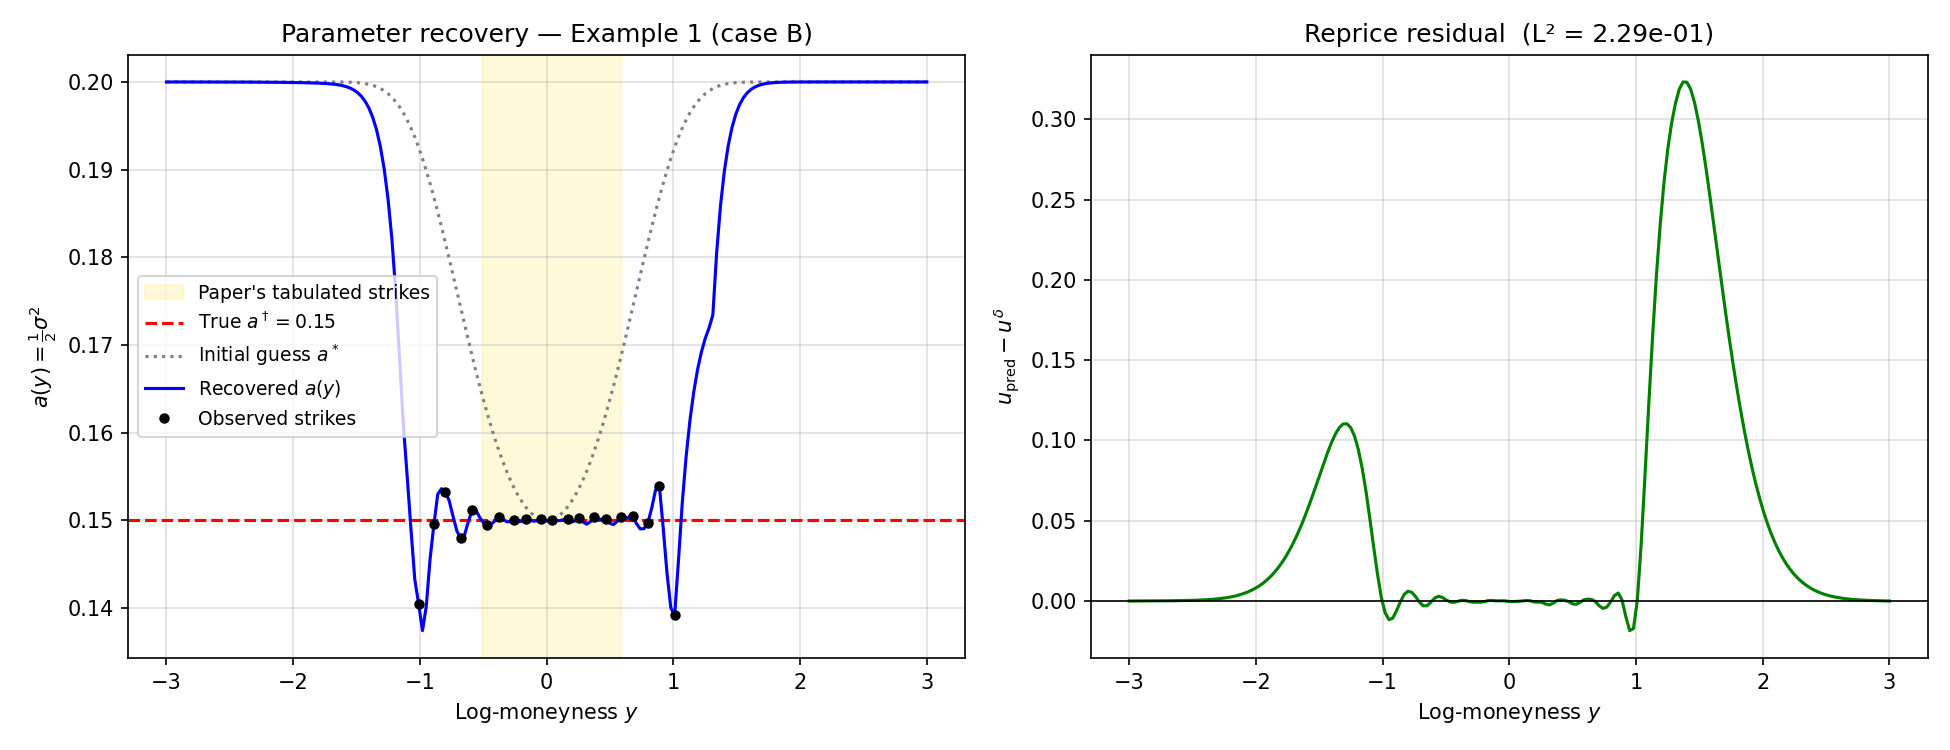
\includegraphics[width=\textwidth]{egger_example1_caseB}
    \caption{
        Example 1 case \emph{B} of \cite{egger2005tikhonov},
        recovering the constant $a(y) = 0.15$ using only 20 strikes.
    }
    \label{fig:egger_ex1_B}
\end{figure}
\begin{figure}[h!]
    \centering
    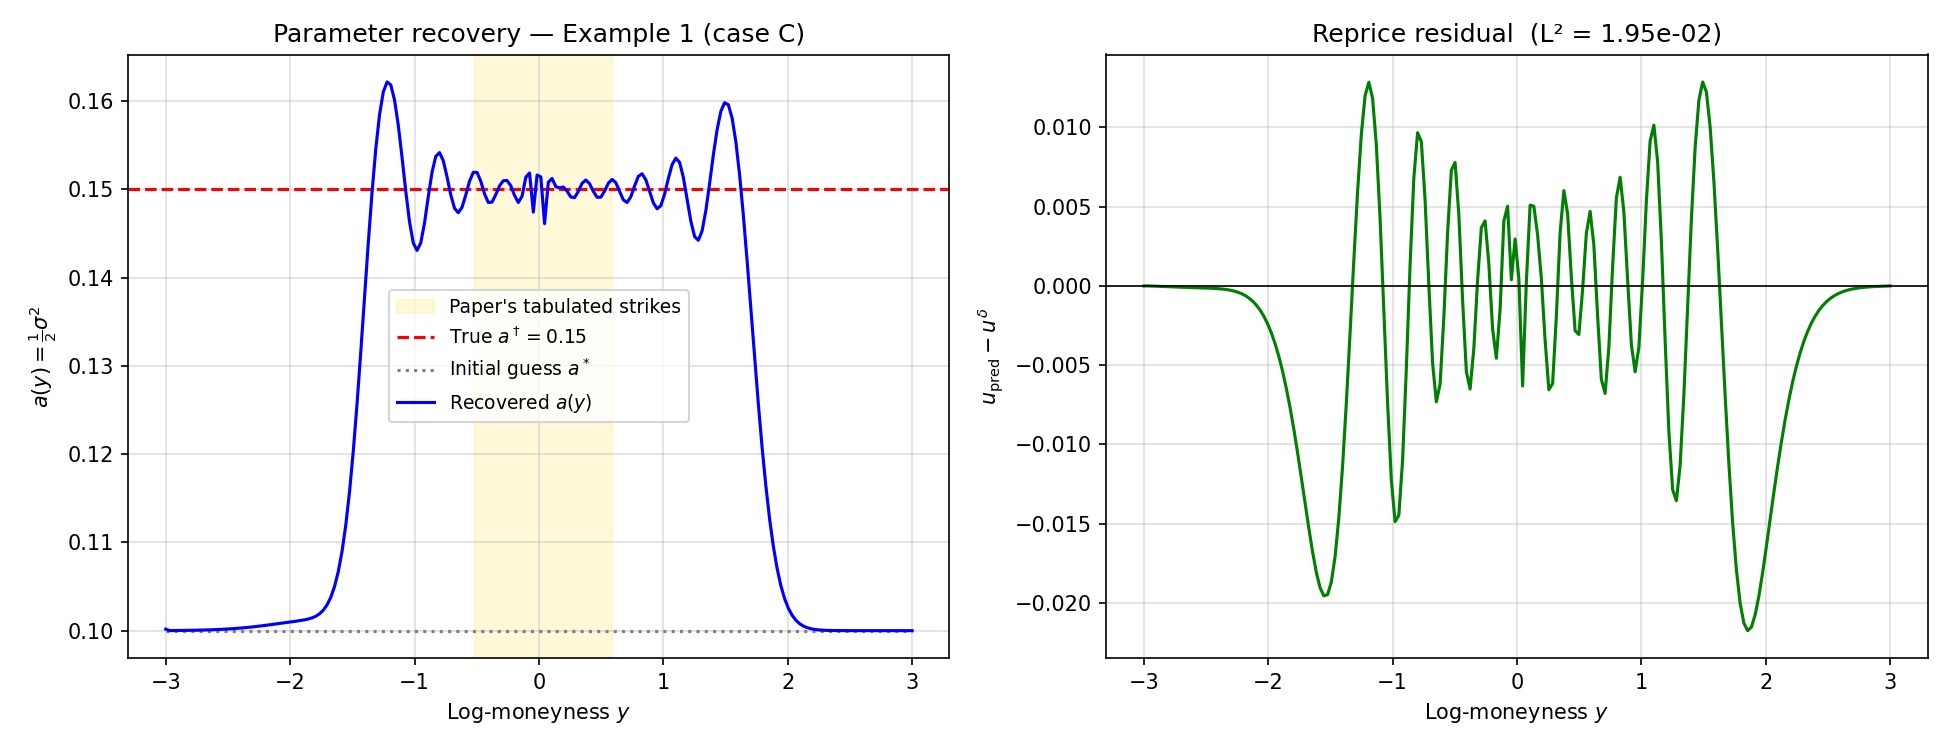
\includegraphics[width=\textwidth]{egger_example1_caseC}
    \caption{
        Example 1 case \emph{C} of \cite{egger2005tikhonov},
        recovering the constant $a(y) = 0.15$ from a poor constant prior $a^* = 0.10$.
    }
    \label{fig:egger_ex1_C}
\end{figure}

While in \emph{D} and \emph{BD} we can see that the noise in the data makes the recovery of the true value more difficult,
we interpreted that the $0.1\%$ noise is applied to the call prices,
thus deep ITM options would have a bigger shock in absolute terms than deep OTM options.
We don't know if that was \emph{Egger's} and \emph{Engl's} approach,
as they mention that the noise would be $ 1\$ $, as the underlying is $1000\$ $,
but that would probably make some deep OTM options to have negative prices,
which is not possible,
thus recovering the true value would be impossible in those cases.

\begin{figure}[h!]
    \centering
    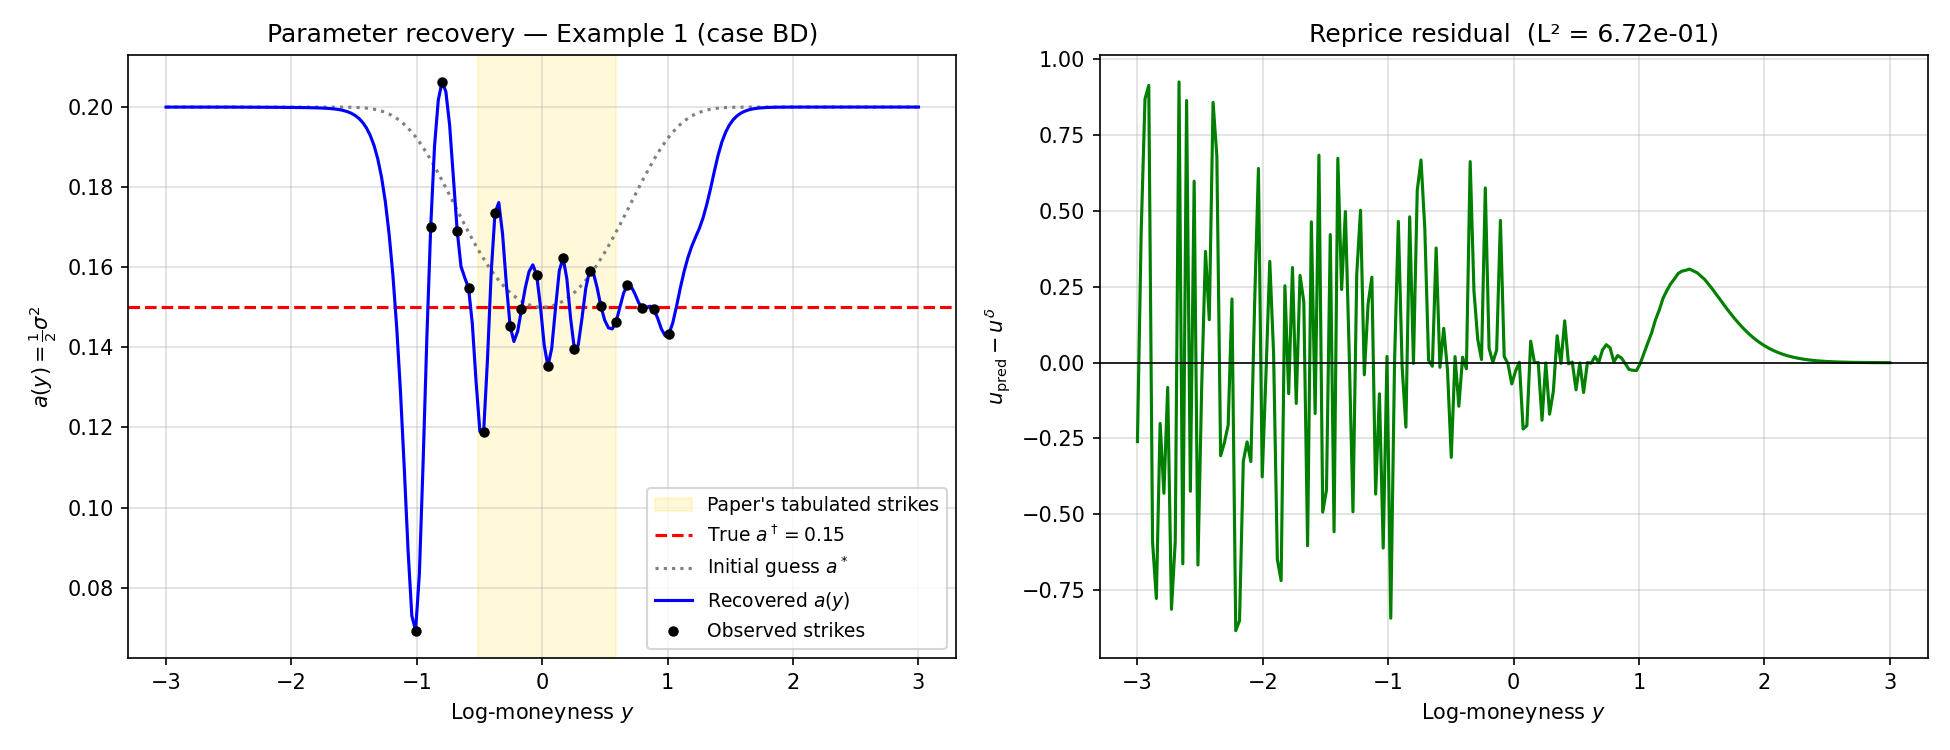
\includegraphics[width=\textwidth]{egger_example1_caseBD}
    \caption{
        Example 1 case \emph{BD} of \cite{egger2005tikhonov},
        recovering the constant $a(y) = 0.15$ from incomplete and noisy data.
    }
    \label{fig:egger_ex1_BD}
\end{figure}

\subsection{Numerical experiment - Example 2}

Example 2 of \cite{egger2005tikhonov} tries to show the importance of regularization.
The set up is similar to example 1,
but its true coefficient $a^\dagger(y)$ is the oscillatory profile near ATM
\begin{equation}\label{eq:egger_ex2_true}
    a^\dagger(y) = 0.15 + 0.05\,e^{-(y+0.3)^2}\sin(2\pi y) + 0.05\,\operatorname{erf}(20 y).
\end{equation}
To avoid an \emph{inverse crime} we generate the synthetic data on a wider domain $[-5,5]$,
with a four-times finer mesh and time step,
and interpolate them onto the coarser reconstruction grid,
so the data do not come from the same discretized operator that is later inverted.
We do it because \cite{egger2005tikhonov} mentions to use a different time-integration scheme for the same reason,
but does not mention the details,
in some of the cases looks like we are getting better reconstruction results and that might be the reason.

We run the paper's five cases.
All use the \emph{a priori} guess
\begin{equation*}
    a^*_1(y) = 0.15 + 0.05 \, \operatorname{erf}(2y),
\end{equation*}
which has the correct wings, except case C,
\begin{itemize}
    \item[(A)] complete, exact data;
    \item[(B)] incomplete data, only $20$ strikes observed;
    \item[(C)] complete, exact data with the poor constant prior $a^* = 0.15$;
    \item[(D)] complete data with $0.1\%$ noise;
    \item[(BD)] incomplete and noisy.
\end{itemize}
For the exact data cases we use a single small $\beta = 10^{-6}$.
Whereas for the noisy cases D and BD select $\beta$ with the decreasing $\beta$ schedule and Morozov discrepancy principle described above,
starting from $\beta_0 = 10^2\delta$ and warm-starting each minimization from the previous one.

Figure \ref{fig:egger_ex2} shows the recovered coefficient for the five cases.
Most exemplifying one is \emph{C},
where we can see the importance of the prior,
the poor constant prior $a^* = 0.15$ is not able to recover the oscillatory true value $a^\dagger(y)$,
specially in the wings where the data is weak and the prior dominates the solution.
\begin{figure}[h!]
    \centering
    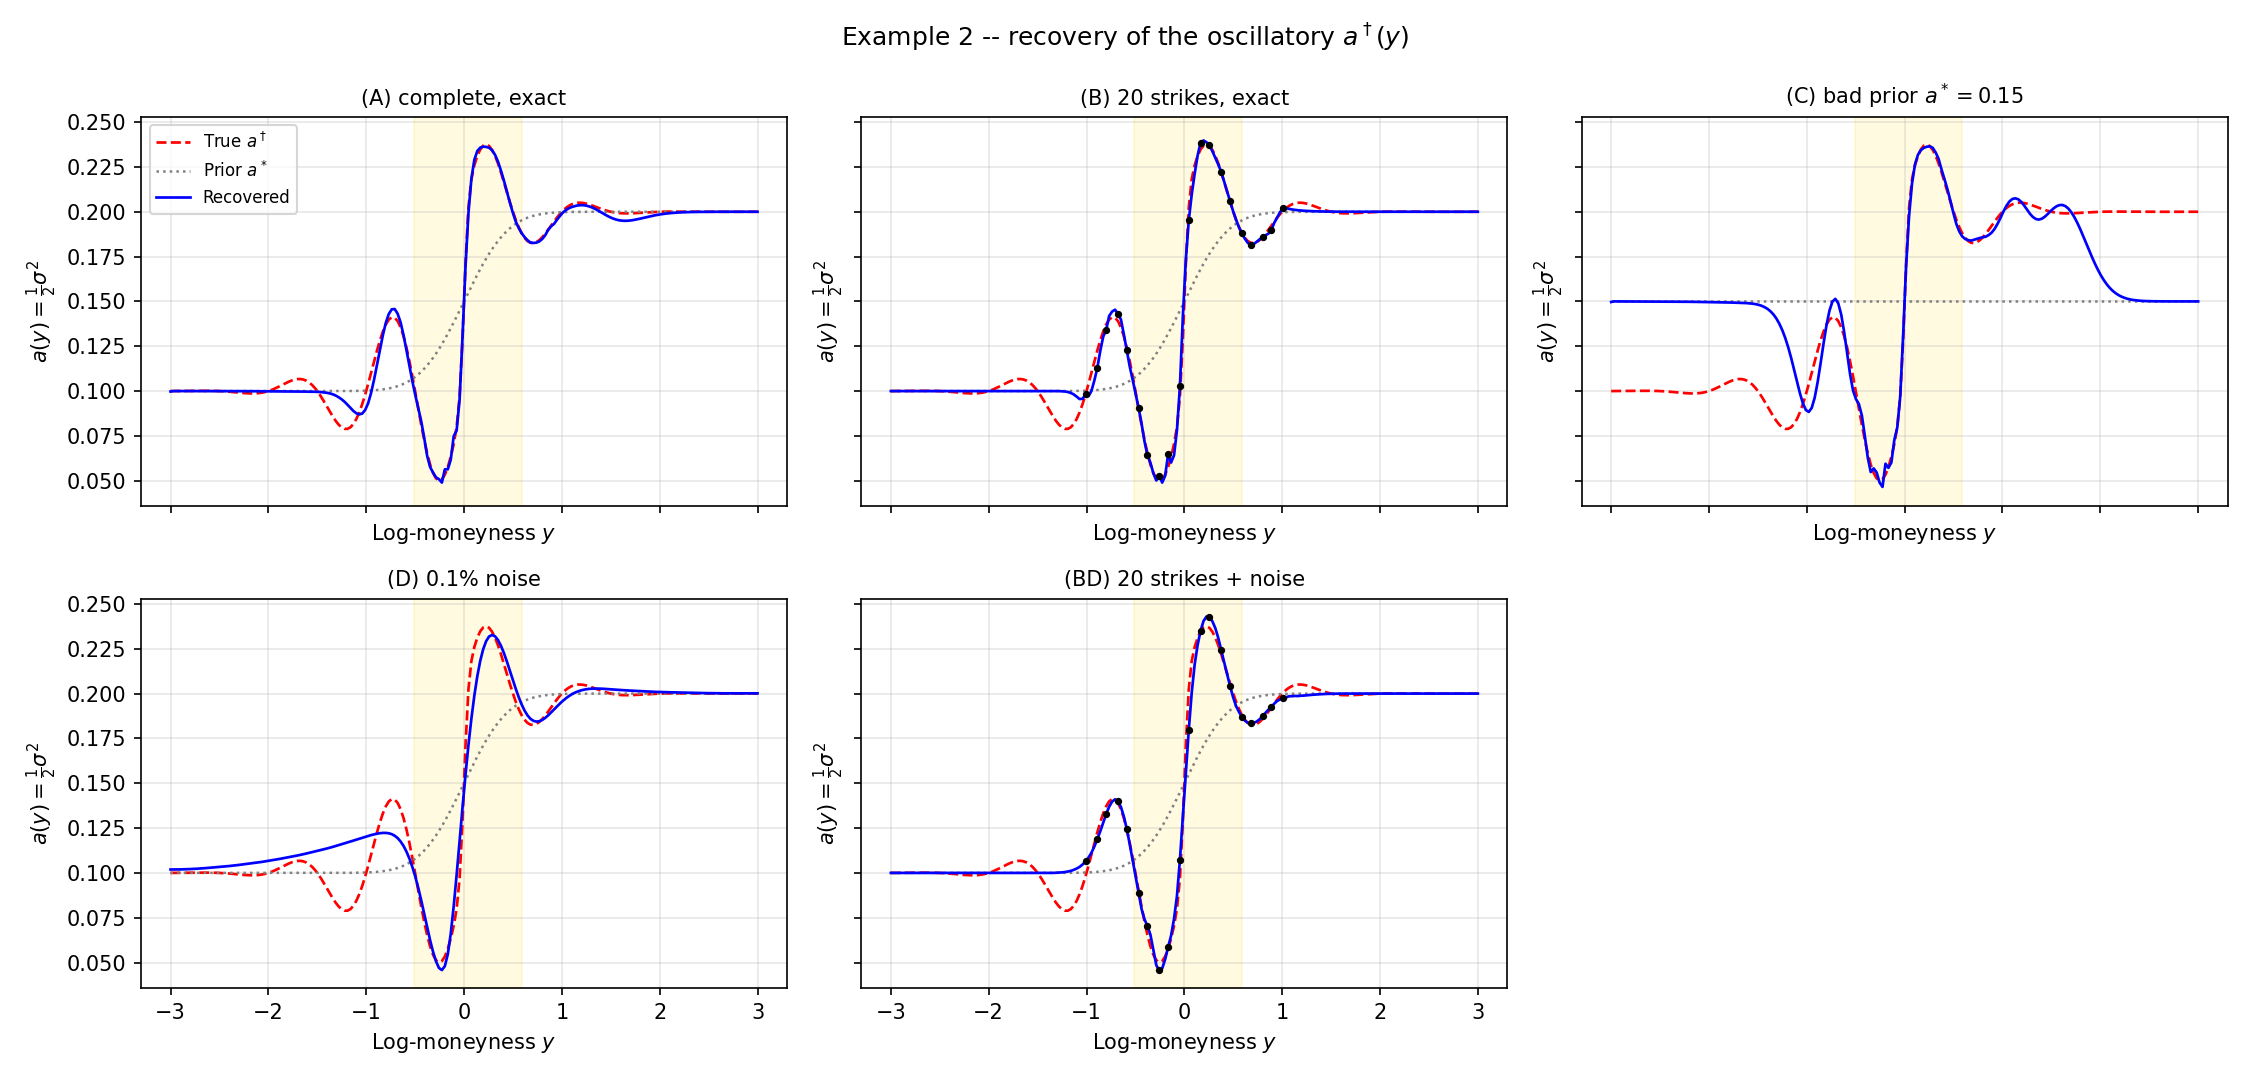
\includegraphics[width=\textwidth]{egger_example2_recovery}
    \caption{Example~2 of \cite{egger2005tikhonov}: recovery of the oscillatory local
             variance $a^\dagger(y)$~\eqref{eq:egger_ex2_true} (red dashed) for the five test
             cases. Blue: recovered $a(y)$; grey dotted: prior $a^*$; black dots (B, BD):
             observed strikes; shaded band: the strikes $K = 600$--$1800$ tabulated in the
             paper.}
    \label{fig:egger_ex2}
\end{figure}

\section{Numerical experiment - a local volatility surface from market data}\label{sec:market_surface}

Examples 1 and 2 use synthetic data and a coefficient that is constant in time. We now
calibrate a full surface $a(y,\tau)$ from real market quotes. This goes past the setting of
Section~\ref{sec:convergence_rates}, where the rate theory assumes a time independent
coefficient: here the unknown is genuinely time dependent, so the surface fit is a numerical
extension rather than a covered case.

The data are SPY European option quotes from 30 April 2026, with spot $S_0 = 720.65$. We use
nine expirations, with maturities $\tau$ from $0.10$ to $0.88$ years. For each expiration the
risk free rate, the dividend yield and the implied volatility come from the pipeline of
Appendix~\ref{app:impl_vol}: the Treasury curve for $r$, put call parity for $q$, and the out
of the money composite for the smile. Each smile is restricted to the moneyness band
$0.8 \le K/S_0 \le 1.2$, where the quotes are liquid. We keep only expirations with at least
twenty five strikes in this band: a sparser expiration is under-determined, and when it sits a
few days from a well-populated one it contributes a redundant thin slice that the fit cannot
resolve and that simply relaxes to a noisy prior.

The surface is held as one spatial slice per maturity, which is the
parametrization~\eqref{eq:coefficient_slices} of Section~\ref{sec:time_dependent_a}: we do not
fit the maturities one at a time nor interpolate between their smiles. The forward equation is
marched once from $0$ to the last maturity, the coefficient taking the value $a_k$ on the $k$th
interval, and the whole time trajectory of the solution is kept and read off at each maturity.
Every observed price is therefore a sample of one and the same evolving solution, and the
unknown is the stack of slices $(a_1,\dots,a_K)$ solved for jointly, at the cost of one forward
solve and one backward adjoint sweep per iteration whatever the number of slices. The
functional minimized is the space and time version~\eqref{eq:surface_functional} announced
there, with $\Omega_j$ the band of strikes quoted at maturity $\tau_j$, the $H^1$ term
smoothing each slice in strike and the $L_2$ term penalizing the jump between consecutive
slices. The triangular
structure noted in Section~\ref{sec:time_dependent_a} is what makes this well posed maturity by
maturity: the earliest expiration constrains the first slice, the next one the second, and so
on. The prior $a^*_k$ of each slice deserves care.
The instinct is to seed it with that maturity's implied variance $\tfrac12\sigma_{\mathrm{iv}}^2$,
but the $H^1$ term penalizes the difference of \emph{slopes} $\partial_y(a_k - a^*_k)$, and by
the factor of two derived below (Section~\ref{sec:factor_two}) the implied skew is only half the
local skew. Such a prior would anchor the reconstruction at the wrong slope and flatten the
recovered skew toward the implied one wherever the data are weak. We instead seed $a^*_k$ with
the local volatility recovered from the smile by inverting the short maturity relation~\eqref{eq:bbf_harmonic},
which on differentiating $y/\sigma_{\mathrm{iv}} = \int_0^y dx/\sigma_{\mathrm{loc}}$ gives
\begin{equation}\label{eq:bbf_inversion}
    \sigma_{\mathrm{loc}}(y) \;=\; \frac{\sigma_{\mathrm{iv}}(y)}
        {1 - y\,\partial_y\sigma_{\mathrm{iv}}(y)/\sigma_{\mathrm{iv}}(y)}.
\end{equation}
This agrees with the smile at the money and doubles its skew there, consistent
with~\eqref{eq:factor_two}; outside the band it is flattened. Interest and dividend enter as
piecewise constant forward rates recovered from the zero rates.

Figure~\ref{fig:egger_surface} shows the result for $\beta_y = 0.1$ and $\beta_\tau = 1$. The
recovered surface has the shape one expects: a pronounced negative skew, with local volatility
close to $0.15$ at the money, near $0.12$ on the upside, and rising sharply on the downside, to
about $0.40$ at the long maturities and much steeper at the short end where the skew is
strongest. Repricing the quotes at the calibrated surface gives a median relative error of
$0.14\%$ across the nine maturities, with the maximum over liquid strikes staying near $1\%$ at
every expiration. This is markedly tighter than the naive prior $a^* = \tfrac12\sigma_{\mathrm{iv}}^2$,
which gives a median of $0.32\%$ and maxima near $2\%$: that prior anchors the skew at half its
correct value, so wherever the quotes carry little information the $H^1$ penalty pulls the
reconstruction off the prices, and the theory-consistent prior~\eqref{eq:bbf_inversion} removes
the bias. As in the synthetic examples, the surface is well determined near the money and
on the downside, where option prices are large and informative, and relaxes towards the prior
on the upside wing, where out of the money call prices are close to zero and constrain the
coefficient only weakly. This is the same ill-posedness of Section~\ref{sec:convergence_rates},
now seen in real data.

The calibrated surface is free of arbitrage, and here the direct approach has a structural
advantage. Because it reproduces the quotes by solving the forward Dupire equation with a local
variance the optimizer keeps strictly positive ($a \ge 10^{-8}$), the output is the price
surface of a genuine diffusion, so the strike and calendar arbitrages of
Section~\ref{sec:no_arbitrage} cannot even be represented. This is unlike the implied volatility
route of Appendix~\ref{app:impl_vol}, where a fitted surface with the slightest butterfly or
calendar violation feeds a negative local variance into the Dupire formula and the
no-arbitrage conditions must be imposed by hand. We verify that the discrete surface inherits
this: the recovered local volatility stays above $0.08$ everywhere, the risk-neutral density
$\partial^2_{KK}\mathcal{C}$ is non-negative across the observed band at every maturity, and the
total implied variance $\sigma_{\mathrm{iv}}^2\tau$ is strictly increasing in maturity at every
moneyness (Figure~\ref{fig:egger_arbitrage}), the two conditions Bergomi records for a local
volatility surface~\cite{bergomi_stochastic_vol}.

\begin{figure}[h]
    \centering
    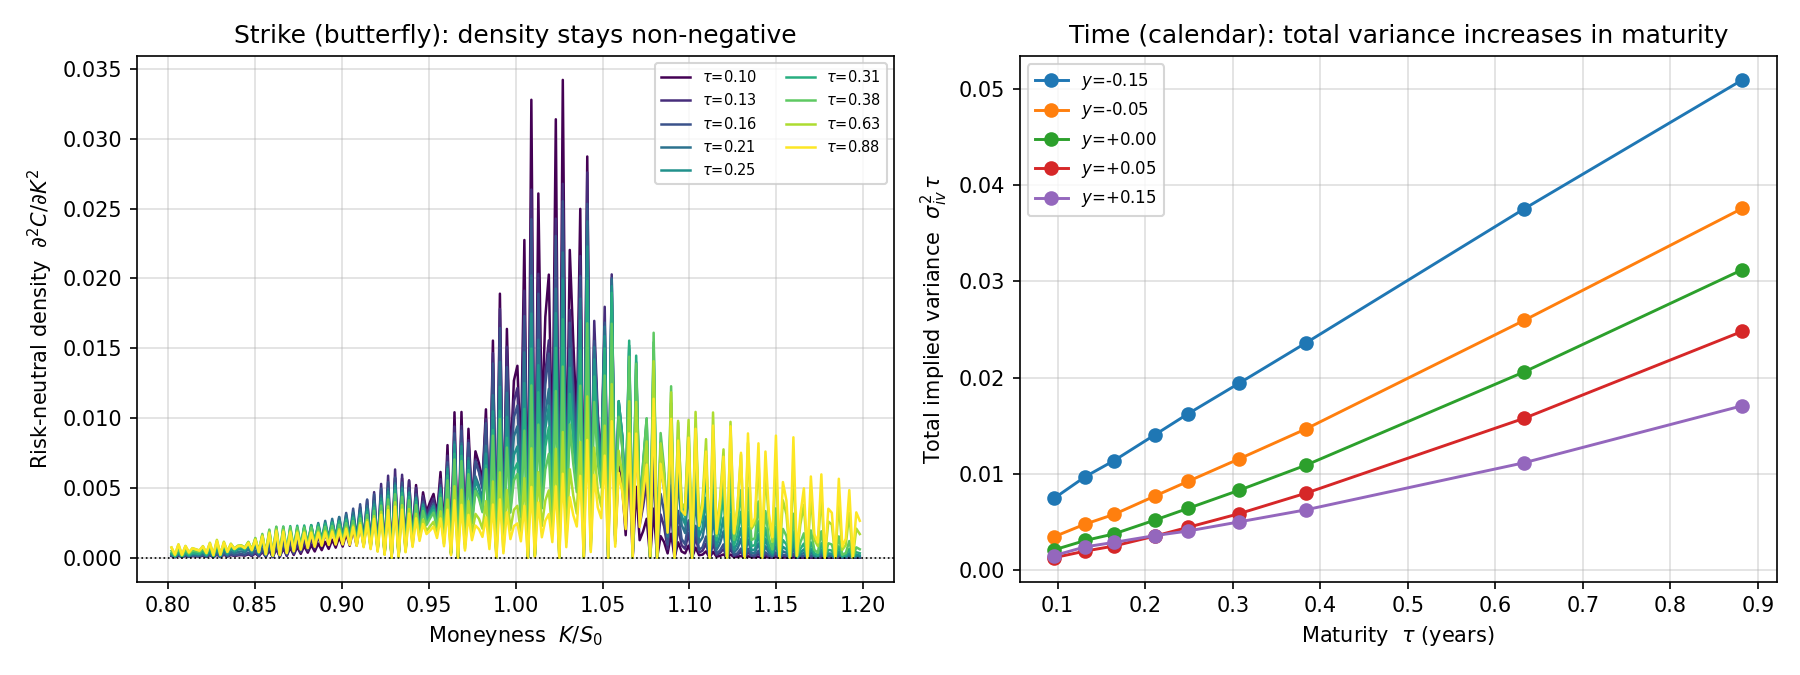
\includegraphics[width=\textwidth]{egger_example7_arbitrage}
    \caption{No-arbitrage check of the calibrated surface of Figure~\ref{fig:egger_surface}.
             Left: the risk-neutral density $\partial^2 \mathcal{C}/\partial K^2$ per maturity,
             non-negative across the observed band (no strike, or butterfly, arbitrage). Right:
             the total implied variance $\sigma_{\mathrm{iv}}^2\tau$ against maturity at fixed
             log-moneyness, increasing everywhere (no time, or calendar, arbitrage).}
    \label{fig:egger_arbitrage}
\end{figure}

One feature of the fit points to the next section. Near the money the recovered local
volatility is visibly steeper in strike than the market implied volatility plotted on the same
axes. This is a definite relation between the two skews, which we make precise next following
Derman and Bergomi.

\begin{figure}[h]
    \centering
    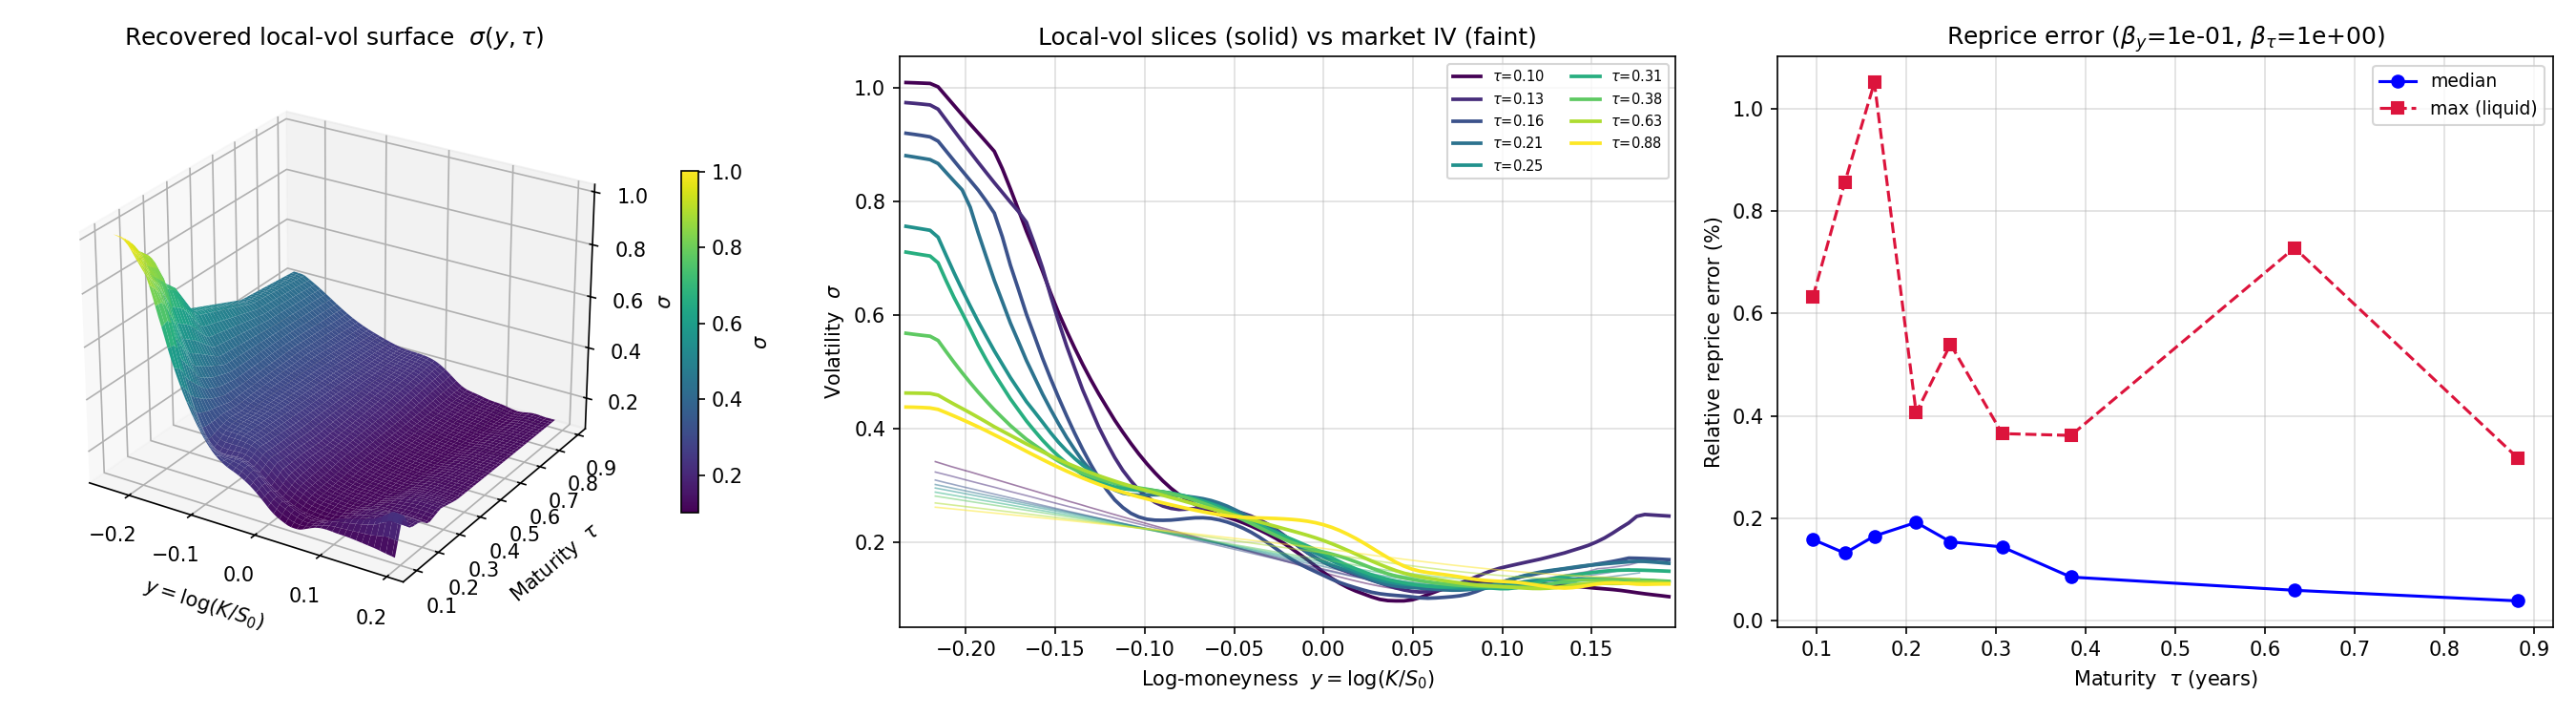
\includegraphics[width=\textwidth]{egger_example4_surface}
    \caption{Local volatility surface calibrated from SPY quotes on 30 April 2026
             ($S_0 = 720.65$, nine maturities), with $\beta_y = 0.1$ and $\beta_\tau = 1$.
             Left: the recovered surface $\sigma(y,\tau)$ as a 3D mesh. Middle: the recovered local
             volatility slices (solid) against each maturity's market implied volatility
             (faint); the local volatility skew is steeper than the implied one. Right: per
             maturity relative reprice error over liquid strikes (market price at least $0.5\%$
             of $S_0$), median and maximum.}
    \label{fig:egger_surface}
\end{figure}

\section{The local volatility skew and the factor of two}\label{sec:factor_two}

The steeper skew seen in Figure~\ref{fig:egger_surface} is not an artefact of the
calibration. It reflects a general relation between the two objects. The implied volatility
$\sigma_{\mathrm{iv}}(K,\tau)$ is the single Black-Scholes number that reprices the quote at
$(K,\tau)$, while the local volatility $\sigma_{\mathrm{loc}}(S,t)$ is the instantaneous
diffusion coefficient the underlying feels at $(S,t)$. The former is an average of the latter
over the paths that reach the strike, so the smile is a smoothed version of the local
volatility and its skew is the flatter of the two. Derman makes this precise near the
money~\cite{derman_vol_smile}.

The clean statement is the short maturity asymptotic of Berestycki, Busca and
Florent~\cite{berestycki_busca_florent}: as $\tau \to 0$ the implied volatility is the harmonic
average of the local volatility over the log-moneyness interval between spot and strike,
\begin{equation}\label{eq:bbf_harmonic}
    \frac{1}{\sigma_{\mathrm{iv}}(y,\tau)}
      \;=\; \frac{1}{y}\int_0^y \frac{dx}{\sigma_{\mathrm{loc}}(x)} \;+\; o(1),
    \qquad y = \log(K/S_0),
\end{equation}
where $\sigma_{\mathrm{loc}}(x)$ is the local volatility at log-moneyness $x$. Writing
$\sigma_{\mathrm{loc}}(x) = \sigma_0 + \sigma_0' x + O(x^2)$ with $\sigma_0 =
\sigma_{\mathrm{loc}}(0)$ and $\sigma_0' = \partial_y \sigma_{\mathrm{loc}}(0)$, the integrand
is $\sigma_0^{-1}(1 - (\sigma_0'/\sigma_0)\,x) + O(x^2)$, so its average over $[0,y]$ equals
$\sigma_0^{-1}(1 - (\sigma_0'/2\sigma_0)\,y) + O(y^2)$. Inverting~\eqref{eq:bbf_harmonic} gives
$\sigma_{\mathrm{iv}}(y) = \sigma_0 + \tfrac12 \sigma_0'\, y + O(y^2)$, that is
\begin{equation}\label{eq:factor_two}
    \left.\partial_y \sigma_{\mathrm{loc}}\right|_{y=0}
      \;=\; 2\,\left.\partial_y \sigma_{\mathrm{iv}}\right|_{y=0}.
\end{equation}
This is Derman's factor of two: at the money the local volatility skew is twice the implied
volatility skew. Bergomi records the same factor on the dynamic side~\cite{bergomi_stochastic_vol}:
in a local volatility model the at-the-money implied volatility moves with the spot at twice the
rate at which it moves with the strike, so the skew stickiness ratio equals two in the short
maturity limit. The static and the dynamic statements are two faces of the same averaging.

We check~\eqref{eq:factor_two} directly on the calibrated surface. For each maturity we fit a
quadratic to the recovered local volatility slice and to the market implied volatility smile in
a narrow window $|y| \le 0.05$ around the money and read the slope at $y = 0$.
Figure~\ref{fig:egger_skew} shows the two skews and their ratio. Near the money the local skew
is about twice the implied skew, with a mean ratio of $2.15$ for maturities below three months.

One objection must be met. The prior~\eqref{eq:bbf_inversion} already builds the factor of two
into the reconstruction, so the agreement could be an echo of the prior rather than a property
of the data. It is not. Rerunning the calibration with the naive prior
$a^* = \tfrac12\sigma_{\mathrm{iv}}^2$, which instead biases the ratio towards one, leaves the
short maturity ratio at $2.17$, essentially unchanged. The factor of two near the money is
recovered from the option prices themselves and is robust to the choice of prior, which is the
real check that the local volatility, and not just the fitted prices, is meaningful. At long
maturities the ratio is prior sensitive, since the quotes thin out and the reconstruction leans
on the prior there, so we do not read a reliable term structure of the ratio from it; this is
consistent in any case with~\eqref{eq:bbf_harmonic} being a short maturity statement.

\begin{figure}[h]
    \centering
    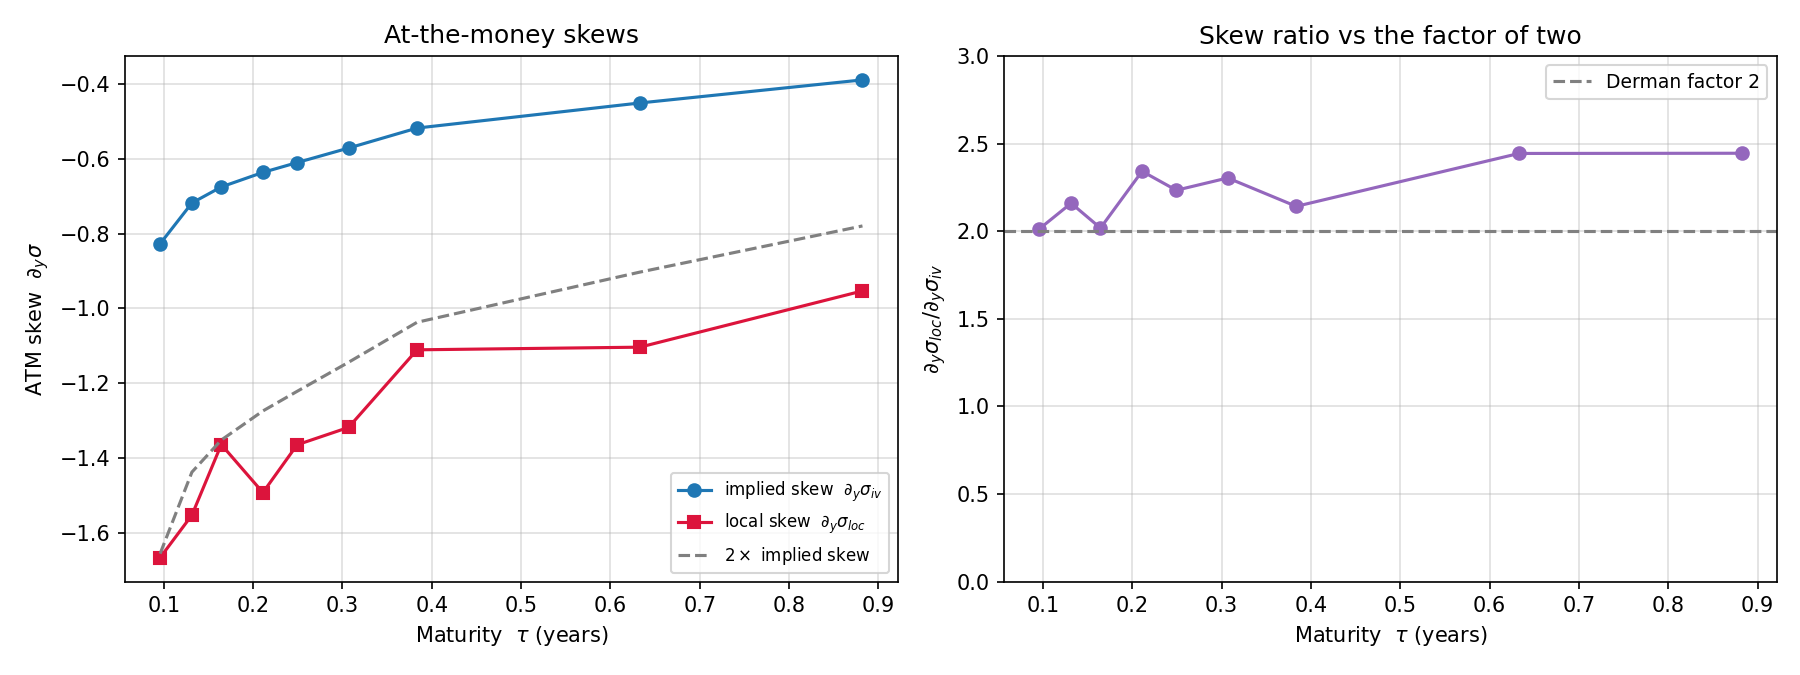
\includegraphics[width=\textwidth]{egger_example5_skew}
    \caption{The Derman factor of two on the SPY surface of Figure~\ref{fig:egger_surface}.
             Left: the at-the-money implied volatility skew, the recovered local volatility
             skew, and twice the implied skew. Right: the ratio of local to implied skew against
             the reference value two. Both skews are read from a quadratic fit in the window
             $|y| \le 0.05$.}
    \label{fig:egger_skew}
\end{figure}

\section{Out of sample test: pricing between quoted maturities}\label{sec:holdout}

The two constructions, the calibrated local volatility surface and the interpolated implied
volatility surface, agree on the quoted maturities by design. They differ on a contract that
falls between them, and that difference is the test that tells them apart. We remove one
interior expiration from the data, the December 2026 quotes at $\tau = 0.63$, and price it out
of sample two ways. The local volatility surface is recalibrated on the remaining eight
maturities and the Dupire equation is propagated across the gap, so the price at $\tau = 0.63$
is a genuine sample of the forward solution rather than an interpolation of the smile. The
implied volatility construction interpolates the total variance $\sigma_{\mathrm{iv}}^2\tau$
linearly in maturity at fixed log-moneyness between the bracketing expirations $\tau = 0.38$
and $\tau = 0.88$, and reads the price off Black-Scholes.

Figure~\ref{fig:egger_holdout} shows the outcome. Both reproduce the held-out smile closely.
Over the liquid strikes the median relative price error is $0.9\%$ for the implied volatility
interpolation and $1.4\%$ for the local volatility surface, so for pricing vanilla options
between quoted dates the interpolation is marginally the more accurate. This is expected, since
interpolating the variance is essentially built to reproduce the smile. The two part company in
the wings. On the upside, where call prices fall towards zero and the relative error is most
demanding, the implied volatility interpolation reaches almost $10\%$, while the local
volatility price stays under $5\%$, since it is tied to the forward equation rather than to a
straight line in variance.

The conclusion is a measured one. For interpolating vanilla prices the two methods are
comparable, with a slight edge to the lighter implied volatility construction near the money
and to the local volatility surface in the wings. The case for the local volatility surface is
not that it prices vanillas more accurately, but that it delivers a full arbitrage-free spot
dynamics, an instantaneous volatility at every $(S,t)$, which a static implied volatility
interpolation does not. That dynamical content, the same object behind Bergomi's skew
stickiness of Section~\ref{sec:factor_two}, is what is needed to price path-dependent and
forward-starting contracts, for which no single implied volatility exists to interpolate.

\begin{figure}[h]
    \centering
    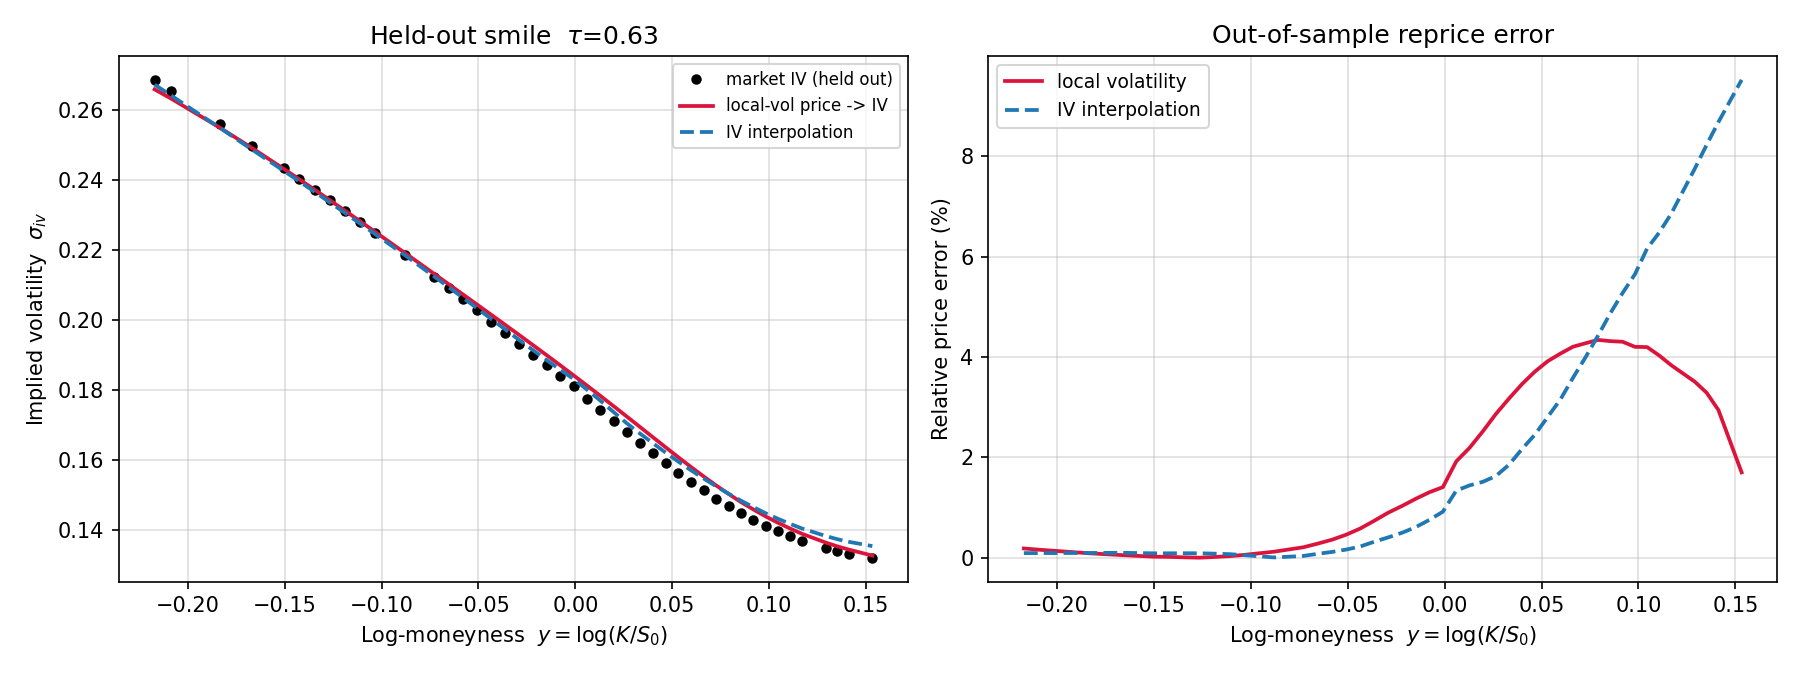
\includegraphics[width=\textwidth]{egger_example6_holdout}
    \caption{Out-of-sample pricing of a held-out expiration (December 2026, $\tau = 0.63$),
             removed from the calibration and bracketed by $\tau = 0.38$ and $\tau = 0.88$.
             Left: the held-out market implied volatilities against the local volatility surface
             price and the implied volatility interpolation, both converted back to implied
             volatility. Right: relative price error over liquid strikes. The two agree near the
             money; in the upside wing the local volatility price is the more stable.}
    \label{fig:egger_holdout}
\end{figure}
\include{8_conclusions}

\appendix
% ----------------------------------
%   Appendix A: Implied Volatility Surface — Implementation Details
% ----------------------------------

\chapter{Implied Volatility Surface - Implementation Details}
\label{app:impl_vol}

This appendix describes the pipeline used to construct the SPY implied volatility
surface shown in Section~\ref{subsec:black_scholes_model},
including the practical difficulties encountered and the assumptions made at each step.
All code lives in \href{https://github.com/M315/TFM/tree/main/scripts/impl_vol/}{Implied Volatility Code} and is reproducible from the cached
market snapshot dated 2026-04-30.

% ----------------------------------
\section{Data}

SPY option chains are fetched via the \texttt{yfinance} library.
We restrict to maturities $4\,\text{wk} \leq T \leq 1\,\text{yr}$ and require a minimum
trading volume of 10 contracts per quote.
When both bid and ask are positive the mid-price is used;
otherwise the last traded price is taken as a fallback (relevant for pre-market snapshots
where the spread is stale but the last price is more informative).
Data for calls and puts are cached separately as \textit{parquet} files so that all
subsequent computations are fully reproducible without network access.

% ----------------------------------
\section{Risk-free rate}

The risk-free rate is taken from the US Treasury par yield curve published daily
by the US Department of the Treasury.
Par yields are available at standard maturities (1M, 2M, 3M, 4M, 6M, 1Y, 2Y, 3Y,
5Y, 7Y, 10Y, 20Y, 30Y) and are converted to continuously-compounded rates via
\begin{equation*}
    r_{\mathrm{cc}} = \ln\!\left(1 + \frac{y}{100}\right),
\end{equation*}
where $y$ is the par yield in percent.
Rates are linearly interpolated (in $T$) between the published nodes and held flat
outside the range.
Figure~\ref{fig:yield_curve} shows the resulting curve on the reference date.

\begin{figure}[h]
    \centering
    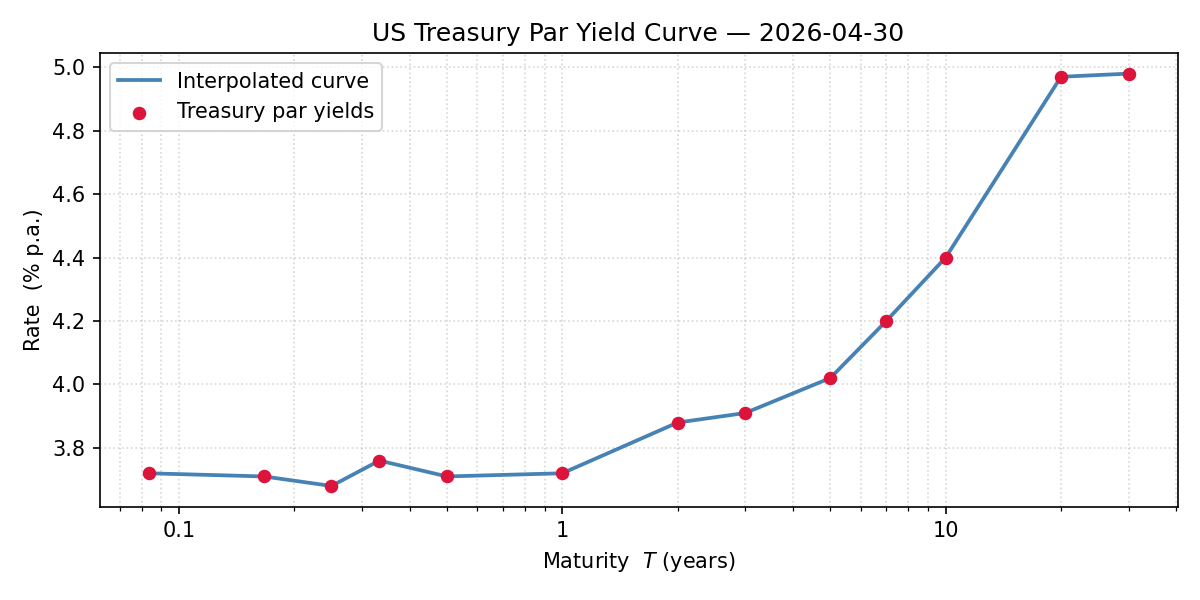
\includegraphics[width=0.72\textwidth]{yield_curve}
    \caption{US Treasury par yield curve on 2026-04-30 (log-maturity axis).
             Red dots are published nodes; the line is the linear interpolant
             used to assign a per-maturity discount rate.}
    \label{fig:yield_curve}
\end{figure}

Note that the risk-free rate could be refined further as the US Treasuries are not strictly risk-free,
as they carry a small credit risk premium.
A better discounting rate for SPY options would be the overnight index swap (OIS) rate rather than the Treasury curve,
but for our purposes the difference is not enough to justify the additional complexity of fetching and processing OIS data.

% ----------------------------------
\section{Dividend yield calibration}
\label{subsec:div_yield_cal}

SPY pays dividends quarterly, so any pricing formula must account for the dividend yield $q$.
Getting $q$ wrong breaks the internal consistency of the surface:
puts and calls at the same strike and maturity imply different volatilities,
producing a visible discontinuity at the money in any composite surface.
We went through three successive approximations before reaching a satisfactory result.

\paragraph{Stage 1 - $q = 0$.}
The simplest assumption is to ignore dividends entirely.
This is equivalent to treating SPY as a non-dividend-paying asset,
which is a standard simplification when the dividend yield is small relative to
the interest rate and the maturity is short.
For maturities beyond a few months, however, cumulative dividends are non-negligible
(SPY's trailing yield is approximately 1.1\%) and the forward price implied by
put-call parity,
\begin{equation*}
    F = S e^{(r - q)T},
\end{equation*}
is overestimated if $q$ is set to zero.
As a result, the Black-Scholes-Merton formula assigns different implied volatilities
to calls and puts at the same strike,
since each type is sensitive to the forward in a different direction.

\paragraph{Stage 2 - Fixed annual yield.}
The natural correction is to use the trailing twelve-month dividend yield reported
by the data provider ($q \approx 1.14\%$ for SPY on the reference date).
This constant is applied uniformly to all maturities.
The surface improves near the money, but the fix is imprecise:
SPY dividends are paid on a quarterly schedule, so the effective yield between
two option expirations depends on how many ex-dividend dates fall within that window.
A short-dated option expiring before the next ex-dividend date carries an effective
$q \approx 0$, while a longer-dated option spanning several dividend payments accumulates
a yield closer to the annual figure.
Applying a single annual constant systematically over-corrects for short maturities
and under-corrects in an uncontrolled way across the term structure.

\paragraph{Stage 3 - Put-Call parity calibration.}
The cleanest approach is to infer $q$ at each expiration directly from market prices
using put-call parity, keeping the Treasury rate $r$ fixed.
For each matched call-put pair at strike $K_i$ and expiration $T$,
put-call parity gives
\begin{equation*}
    C_i - P_i = S e^{-qT} - K_i e^{-rT}.
\end{equation*}
Defining the cost-of-carry forward $F = S e^{(r-q)T}$ and multiplying both sides
by $e^{rT}$ yields an implied forward per pair,
\begin{equation*}
    F_i = (C_i - P_i)\,e^{rT} + K_i,
\end{equation*}
where $q$ is encoded inside $F_i$ rather than appearing explicitly.
Taking the median over the relevant pairs at a given expiration yields a robust
forward estimate $\tilde{F}$, and inverting $\tilde{F} = S e^{(r-q)T}$ gives
\begin{equation*}
    q = r - \frac{\ln(\tilde{F}/S)}{T}.
\end{equation*}

A key implementation choice is \emph{which pairs to include}.
Put-call parity holds model-free for any European options,
but the quality of the forward estimate depends on how cleanly each leg is priced.
For a strike $K < S$ the call is in-the-money and the put is out-of-the-money;
for $K > S$ the roles are reversed.
Deep in-the-money options are significantly less liquid:
their price is dominated by intrinsic value, the bid-ask spread is wide relative
to the time value, and last-trade prices can be hours stale.
Feeding these pairs into the forward estimate biases $\tilde{F}$ toward noisy values.

We therefore restrict the calibration to near-ATM pairs satisfying
$|K/S - 1| \leq 0.05$ (i.e.\ strikes within $\pm 5\%$ of the current spot).
In this band, both the call and the put are close to at-the-money;
both legs have tight spreads and meaningful open interest,
and the time value is large relative to the bid-ask noise.
The median over these pairs (rather than the mean or a least-squares fit)
guards against the occasional stale quote even in the near-ATM region.
If fewer than two near-ATM pairs are available the constraint is relaxed to all matched pairs.

Since $r$ is fixed from the Treasury curve, there is only one free parameter per
expiration, which avoids the instability of simultaneously fitting both $r$ and $q$.
Calibrated values are bounded to $q \in [-0.02, 0.10]$; if the result is outside
this range (a sign of too few matched pairs or erroneous data), the provider value
is used as a fallback.

The resulting term structure shows $q \approx 0$ for near-term expirations
(the next quarterly dividend has not yet been declared within the window)
and a gradual convergence to the trailing annual yield for longer maturities,
which is economically consistent with the quarterly payment schedule.

Figure~\ref{fig:atm_gap} illustrates the three stages for the December 2026 expiration
($T \approx 0.63$ yr), where the effect of the dividend yield is large enough to be
clearly visible.
Each panel overlays the put-implied and call-implied volatility curves across the
full strike range.
With $q = 0$ (Stage 1) the two curves diverge significantly and the level is
shifted upward for OTM puts and downward for OTM calls.
With a fixed annual $q$ (Stage 2) the ATM region improves but the term-structure
mismatch remains.
With the PCP-calibrated $q$ (Stage 3) the two curves sit on top of each other
near the money, confirming that the composite surface can be joined smoothly.
The residual divergence at deep in-the-money strikes visible in all three panels
is due to liquidity issues (wide bid-ask spreads, stale prices) rather than the
dividend yield assumption, and is removed by restricting the composite to
out-of-the-money quotes only.

\begin{figure}[h]
    \centering
    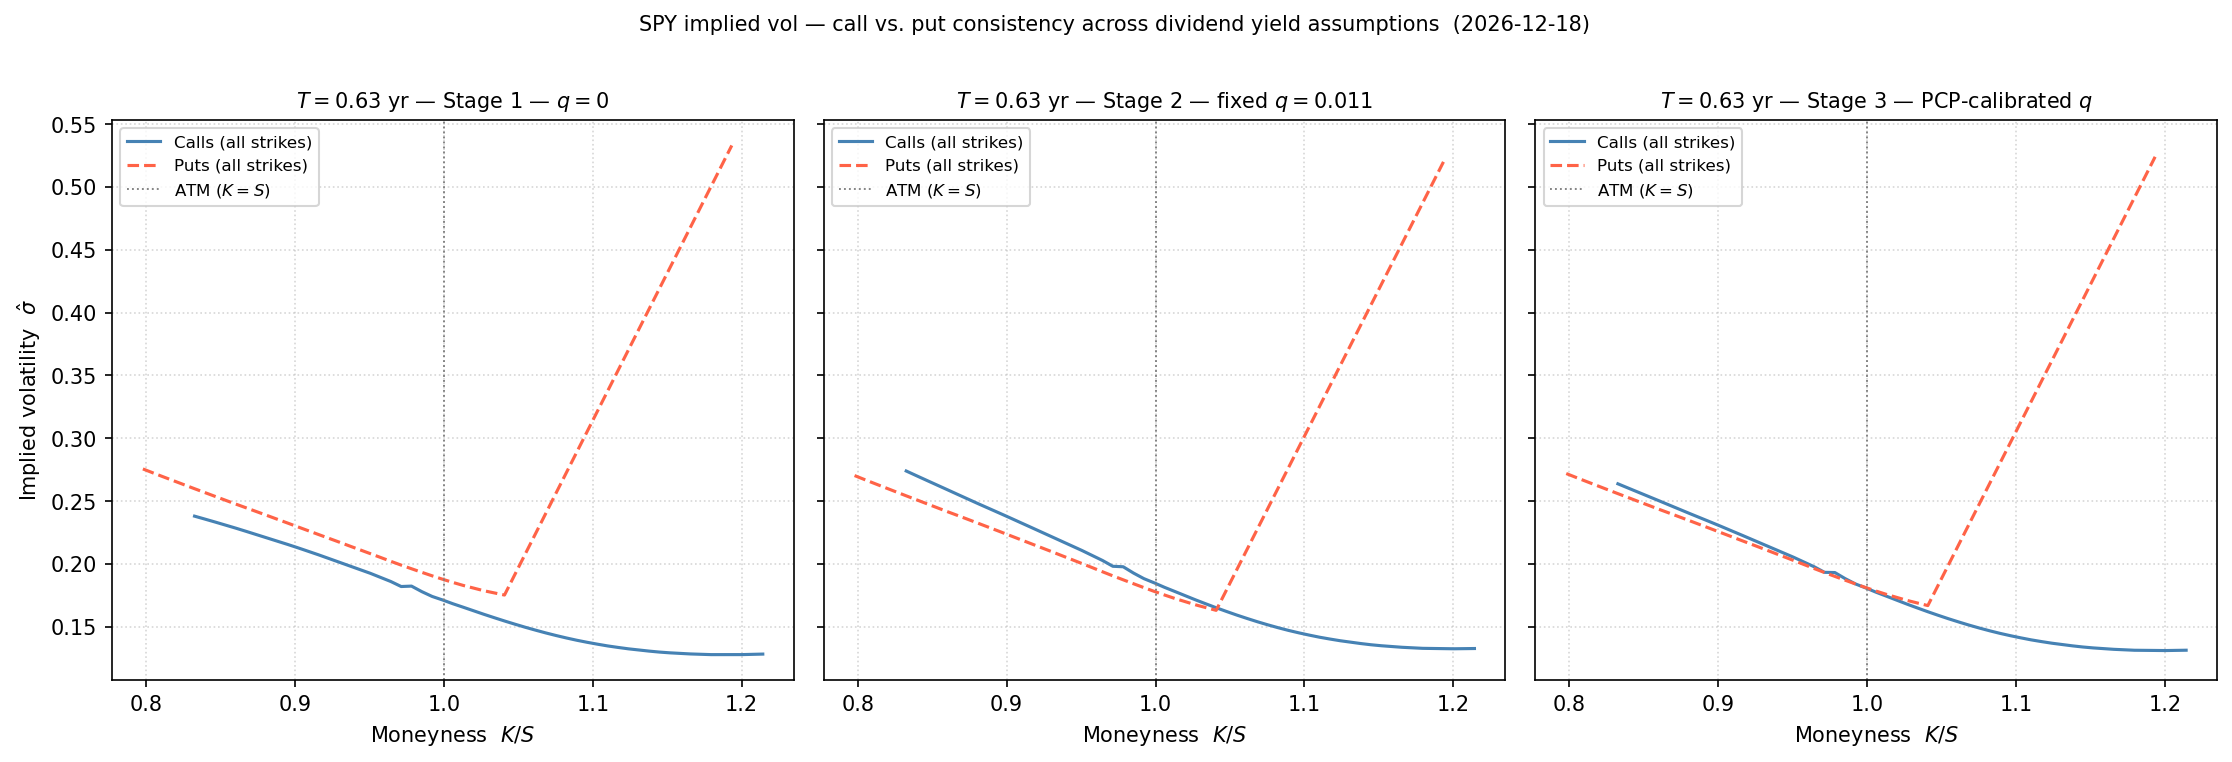
\includegraphics[width=\textwidth]{annex_atm_gap}
    \caption{Call-implied (solid blue) and put-implied (dashed red) volatility across
             all available strikes at the December 2026 expiration ($T \approx 0.63$ yr),
             under three dividend yield assumptions.
             Stage 1 ($q=0$): curves diverge sharply — the forward is overestimated,
             shifting call and put IVs in opposite directions.
             Stage 2 (fixed annual $q$): improved near ATM, but the flat term structure
             leaves systematic errors for maturities where the true $q$ differs from
             the annual average.
             Stage 3 (PCP-calibrated $q$ from near-ATM pairs): the two curves coincide
             in the OTM region, where both legs are liquid.
             The residual divergence far from ATM (deep ITM options) is a liquidity
             artefact — those strikes are excluded from the composite surface.}
    \label{fig:atm_gap}
\end{figure}

% ----------------------------------
\section{OTM composite construction}

Once $r$ and $q$ are consistent with market prices, the composite surface is formed
by taking out-of-the-money options only:
OTM puts ($K < S$) for the left wing and OTM calls ($K \geq S$) for the right wing.

The rationale is that in-the-money options are significantly less liquid than
their out-of-the-money counterparts: ITM bids tend to be stale, spreads are wide,
and the option price is dominated by intrinsic value, so a small absolute pricing
error translates into a large relative error in the time value — and therefore a
large error in the inverted implied volatility.
This is visible in Figure~\ref{fig:atm_gap}: the divergence between call and put
IV curves away from the money persists even in Stage~3, not because $q$ is wrong
but because deep-ITM prices are unreliable.

Figures~\ref{fig:iv_calls} and \ref{fig:iv_puts} show the full call and put surfaces
(all strikes, no ITM filter) to illustrate the noise.
The clean composite (Figure~\ref{fig:iv_surface}) is obtained after restricting to
$0.75 \leq K/S \leq 1.25$ and keeping only the OTM leg for each option type.

\begin{figure}[h]
    \centering
    \begin{minipage}{0.49\textwidth}
        \centering
        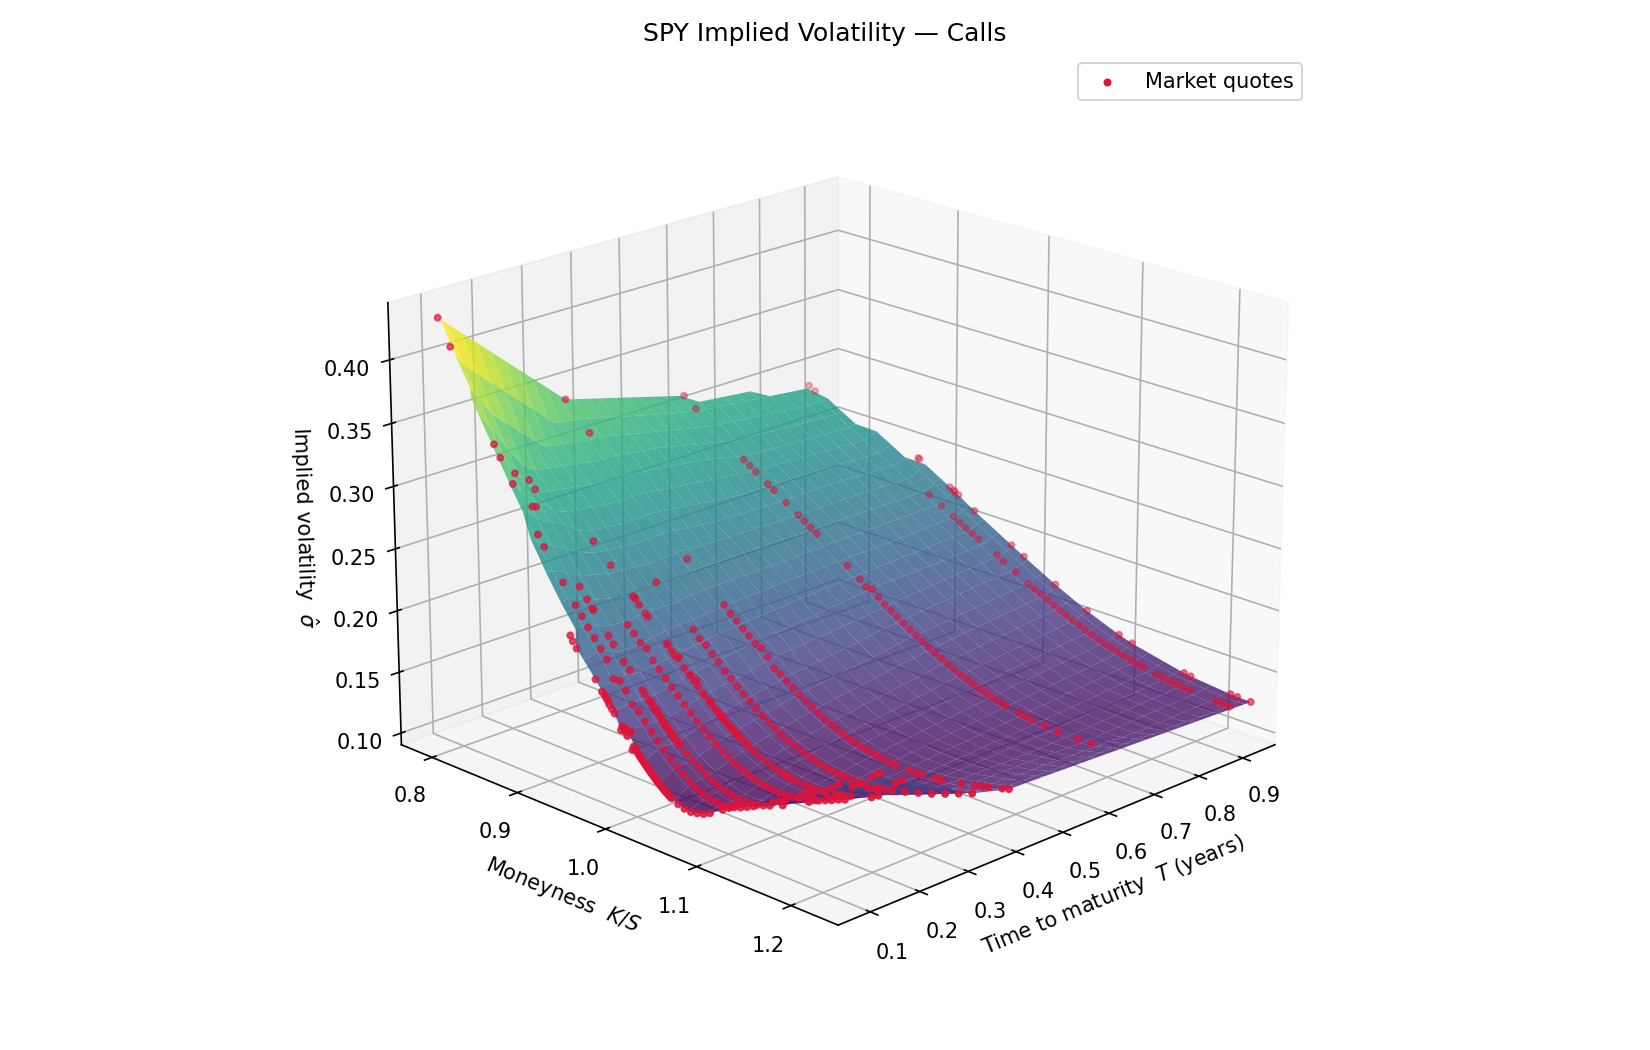
\includegraphics[width=\textwidth]{iv_calls}
        \caption{IV surface from all call quotes (including deep ITM, $K \ll S$).
                 Deep ITM calls carry noisy implied volatilities due to wide spreads
                 and stale prices.}
        \label{fig:iv_calls}
    \end{minipage}
    \hfill
    \begin{minipage}{0.49\textwidth}
        \centering
        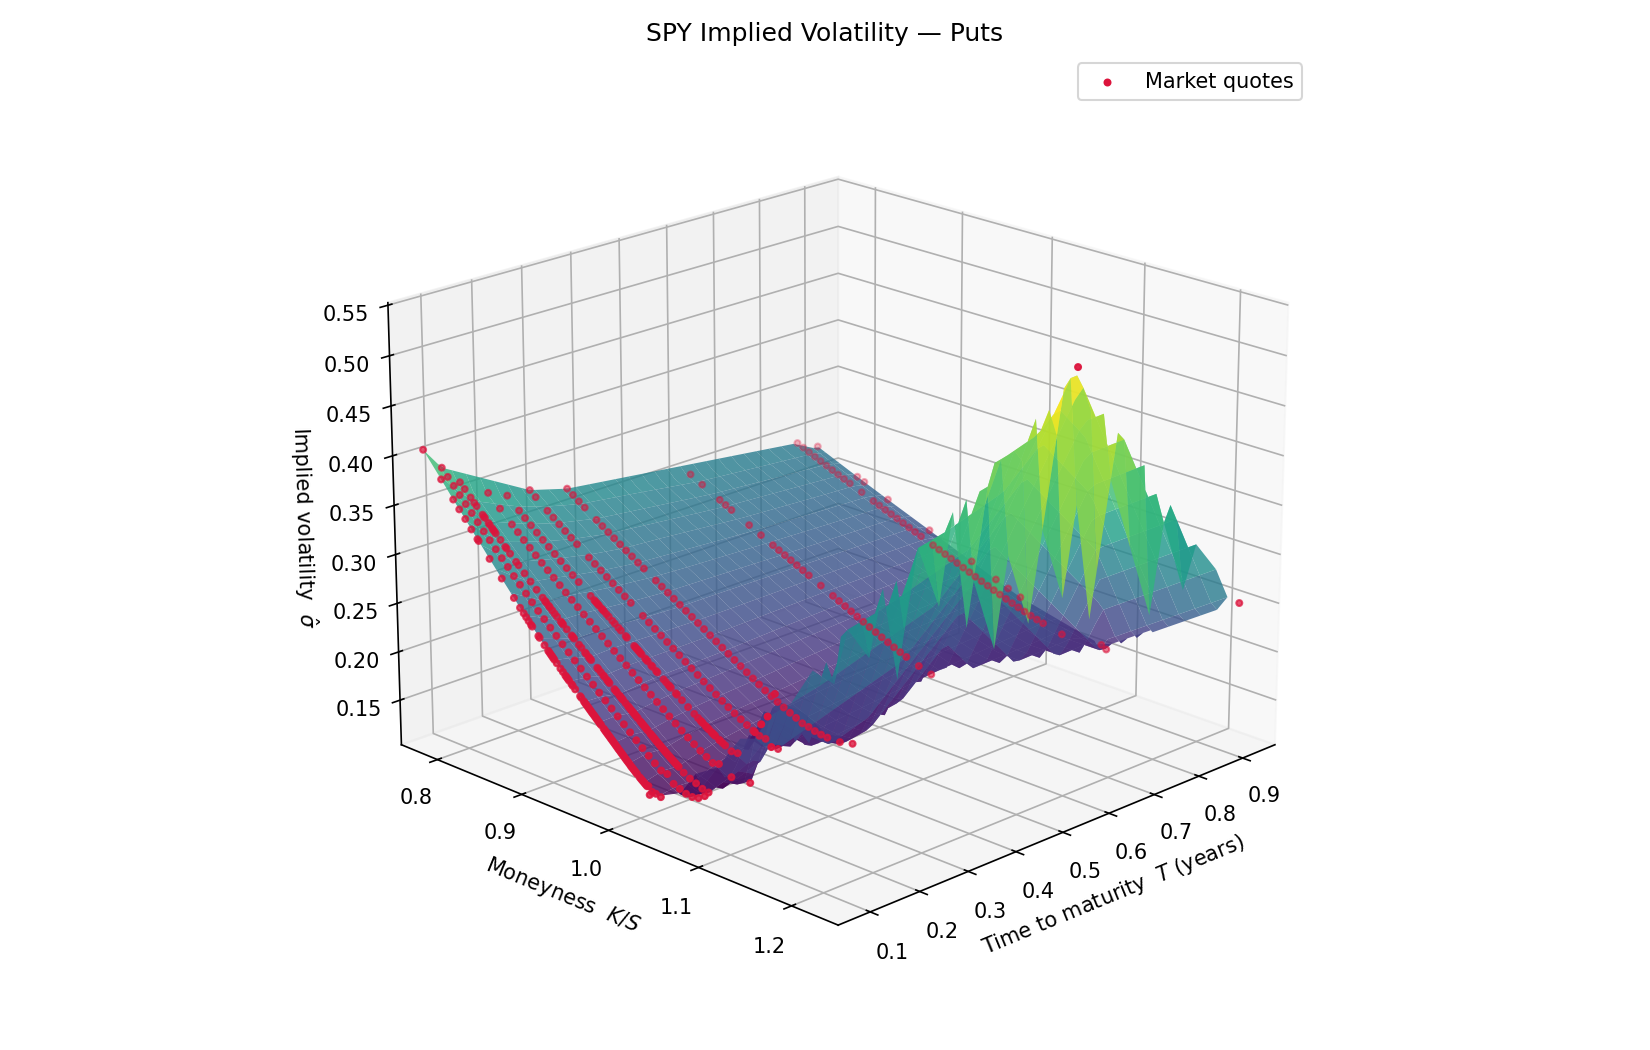
\includegraphics[width=\textwidth]{iv_puts}
        \caption{IV surface from all put quotes (including deep ITM, $K \gg S$).
                 Same liquidity issue for strikes far above the spot.}
        \label{fig:iv_puts}
    \end{minipage}
\end{figure}

% ----------------------------------
\section{Expiration selection}

SPY has a dense cluster of weekly expirations in the short end (roughly 1-8 weeks).
Including all available expirations would over-weight this region and produce a surface
that appears smooth in absolute maturity but poorly samples the longer end.
To obtain a balanced representation, the full maturity range is divided into
$N = 10$ log-spaced bins; within each bin the expiration with the highest combined
open interest (calls plus puts) is kept.
This ensures that liquidity guides the selection and that the resulting sample
is approximately uniform in $\log T$, which is the natural scale on which the
term structure of volatility varies.

% ----------------------------------
\section{Summary of assumptions}

For reference, the key modelling assumptions are:
\begin{itemize}
    \item \textbf{European exercise}: SPY options are technically American-style.
          The early-exercise premium is small for an index ETF with a low continuous yield
          and is neglected here; the BSM formula is used as an approximation.
    \item \textbf{Continuous dividends}: actual SPY dividends are discrete quarterly
          payments. The PCP calibration implicitly converts them into a continuous yield
          that is consistent with the current option prices, which is the standard
          market convention.
    \item \textbf{Moneyness filter} $0.75 \leq K/S \leq 1.25$: strikes outside
          this range are too illiquid to contribute reliable IV observations.
    \item \textbf{Volume filter}: quotes with fewer than 10 contracts of daily volume
          are excluded.
    \item \textbf{Single snapshot}: the surface is computed from a single end-of-day
          snapshot; intraday bid-ask movements are not captured.
\end{itemize}

% ----------------------------------
%   Appendix B: Local Volatility Surface — Implementation Details
% ----------------------------------

\chapter{Local Volatility Surface - Implementation Details}
\label{app:local_vol}


This appendix collects the implementation of the local volatility calibration of
Chapter~\ref{cha:cal_local_vol} and the decisions taken along the way that the main text
states without justifying.
All code lives in \href{https://github.com/M315/TFM/tree/main/scripts/local_vol_egger/}{Local Volatility Code}
and runs from the same cached SPY snapshot dated 2026-04-30
used throughout Appendix~\ref{app:impl_vol}.
The first sections describe the discrete problem that is actually solved, the domain, the
parametrization of the surface, the observation operator and the gradient sweep.
The later ones record the choices that could reasonably have been made differently, the prior,
the term structure, the selection of expirations, the regularization parameters and the
normalization of the unknown.

% ----------------------------------
\section{Discretization and computational domain}
\label{subsec:discretization_details}

The discretization is the one announced in Section~\ref{sec:variational_forms}, $P_1$ elements
in $y$ and backward Euler in $\tau$. What the main text leaves open is the size of everything.

The spatial domain is not fixed in advance, it is read off the data. Each kept expiration
contributes the log-moneyness range of its quoted strikes inside the band
$0.8 \le K/S_0 \le 1.2$, the union of those ranges is $y \in [-0.217,\,0.177]$, and the
computational domain is that union padded by $0.25$ on each side,
$y \in [-0.467,\,0.427]$, that is strikes from $0.63\,S_0$ to $1.53\,S_0$.
The pad is what separates the artificial boundary from the data.
Its width is about $1.8$ standard deviations of the longest maturity,
$\sigma\sqrt{\tau} \approx 0.14$ at $\sigma = 0.15$ and $\tau = 0.88$,
so whatever error we commit at the boundary is damped by the diffusion before it reaches the
observed band. Widening it further only buys solve time, since the coefficient out there is
constrained by no quote at all.

The mesh is uniform, $199$ elements and therefore $200$ nodes, a spacing of
$h \approx 4.5\times 10^{-3}$ in $y$, under half a percent in strike and finer than the quoted
strike spacing everywhere in the band. Time is divided into $300$ steps up to the last
maturity, $\Delta\tau \approx 2.9\times 10^{-3}$ years, close to one calendar day.

Backward Euler is a deliberate choice over Crank-Nicolson. Crank-Nicolson is second order in
time, but it is not strongly damping: its amplification factor tends to $-1$ for the stiff
modes, so a non-smooth initial condition leaves oscillations that decay only slowly. Our
initial condition is the call payoff, whose kink at $y = 0$ excites exactly those modes, and
the oscillations are worst in the second derivative in strike, which is the quantity carrying
the information about $a$. The standard cure is a Rannacher startup of a few implicit steps
\cite{giles_carter_crank_nicolson}. We use implicit Euler throughout instead, which is
uniformly damping at first order, because the time error is not the binding constraint here:
Table~\ref{tab:discounted_pde} below measures it at a day-sized step as
$5\times 10^{-2}$ dollars on a spot of $720$, a relative $10^{-4}$, an order of magnitude
below the reprice errors we report.

The solver works in dollars, not in the normalized price $u = C/S_0$ of
Section~\ref{sec:change_variable}. The equation is linear so the two differ by a constant
factor and describe the same coefficient, but the data term scales as $S_0^2$ while
$\beta\|a - a^*\|^2_{H^1}$ does not, so $\beta$ is tied to the scale of the prices. The values
quoted below are for prices in dollars at a spot of $720$, and they cannot be carried to
another underlying, or to the normalized form, without rescaling.

The boundary conditions are Dirichlet at both edges. The limits recorded
in~\eqref{eq:inverse_pde_2}, intrinsic value on the left and zero on the right, hold as
$M \to \infty$ and are too crude at a pad of $0.25$, where a call struck at $0.63\,S_0$ is
still worth appreciably more than its intrinsic value at long maturity. We instead evaluate
the Black-Scholes price at the two edge strikes, using that maturity's zero rate and dividend
yield and a wing volatility interpolated across the term structure from the extreme quoted
strike of each smile. This is exact whenever the smile is flat outside the quoted band, which
is the same assumption already built into the flat extension of the prior. At $\tau = 0$ the
boundary value is the payoff, so the data are continuous at the corner.

% ----------------------------------
\section{The surface as a stack of time slices}
\label{subsec:slice_parametrization}

The unknown is the stack of spatial slices of~\eqref{eq:coefficient_slices}, one per quoted
maturity. With eleven maturities and $200$ nodes that is $2\,200$ numbers, held as a single
flat vector, which is what the optimizer sees and what the bound constraints act on.

The slice boundaries have to live on the time grid, so each maturity is snapped to the nearest
time level, and if two maturities land on the same level the later one is pushed forward by
one step. On this data the eleven maturities map to distinct levels and the longest lands
exactly on the final step. The maturity the model prices is therefore displaced from the
quoted one by at most half a step, about half a day, and we do not correct for it: the
displacement is well inside the uncertainty of an end of day quote.

Slice $k$ then covers $(\tau_{k-1},\tau_k]$ and the observation at $\tau_k$ is read off the
trajectory at exactly the level where slice $k$ ends. This is what makes the triangular
structure of Section~\ref{sec:time_dependent_a} exact in the discrete problem: the first
expiration sees only the first slice, the second one the first two, and so on.

The optimizer imposes $a \ge 10^{-8}$ and no upper bound, although the admissible
set~\eqref{eq:admissible_set} carries one. The lower bound is the one that matters, it keeps
the operator parabolic and the recovered volatility real, and it is what makes the calibrated
surface arbitrage-free by construction.

% ----------------------------------
\section{The residual, and how a smile becomes data}
\label{subsec:observation_operator}

The misfit is the finite element $L^2$ norm over the observed band, not a sum of squared
errors over the quotes. Each expiration's call prices are interpolated linearly onto the mesh
nodes, and the difference against the computed price is multiplied by the $\{0,1\}$ indicator
of the nodes lying inside that expiration's quoted range. Because the mask is a projection,
$P^2 = P$, the same masked residual is simultaneously the integrand of the data term and the
source injected into the adjoint sweep, and no separate transpose has to be worked out.

The consequence of measuring the misfit in a continuum norm is that quotes are weighted by
mesh spacing rather than by how many of them there are. The expiration with $116$ strikes in
the band and the one with $46$ contribute the same integrated weight over the same interval of
moneyness, and a region where the chain quotes every dollar does not outweigh one where it
quotes every five. A plain sum over quotes would tilt the fit toward the densely quoted
expirations and toward the money, for no modelling reason.

The mask is a hard cut at the ends of each quoted range. Nothing outside is fitted, so the
coefficient in the wings is set by the penalty alone, which is exactly the behaviour visible
in the recovered slices of Figure~\ref{fig:egger_slices}.

% ----------------------------------
\section{The gradient in a single backward sweep}
\label{subsec:gradient_sweep}

One evaluation of the functional and its gradient is the following sequence.

\begin{enumerate}[label=(\roman*)]
    \item March the forward equation from $\tau = 0$ to the last maturity, storing the whole
          trajectory. Here that is $301$ states of $200$ values, so everything fits in memory
          and no checkpointing is needed.
    \item At each observed level, form the masked residual, accumulate its squared norm into
          the data term, and set the residual aside as an injection.
    \item March the adjoint equation backward from the last level, started from the last
          maturity's residual.
    \item At each step, after solving for the new adjoint state, assemble that step's
          contribution to the gradient and add it to the slice that owns the step.
    \item Only then, add the residual observed at that level to the adjoint state.
    \item Add the gradient of the penalty.
\end{enumerate}

The order of (iv) and (v) is the part that is easy to get wrong. Injecting the residual of
$\tau_j$ before taking the step's gradient contribution would let the price quoted at $\tau_j$
feed the coefficient on $(\tau_j,\tau_{j+1}]$, that is, it would make an option depend on the
volatility after its own expiry. Taking the contribution first keeps the dependence causal and
reproduces the triangular structure at the discrete level.

Two further points deserve recording.

The gradient is assembled directly as a linear form against the test functions and stopped
there, with no mass matrix solve. Solving $M g = b$ would instead return the Riesz
representative of the derivative in $L^2$, which is the natural gradient of the continuous
problem, whereas the assembled vector $b$ is the derivative with respect to the nodal
coefficients. Both are legitimately called the gradient, in different inner products, and
mixing the two is the usual way to obtain a gradient test that passes on one mesh and fails on
the next. We use the coefficient version everywhere, and the penalty gradient is assembled to
match, as $2\beta(M + K)(a - a^*)$ with $M$ and $K$ the mass and stiffness matrices, so the
two terms of the functional are differentiated in the same sense. It is also the version
L-BFGS-B expects, since its line search and its box constraints act on the coefficients.

What is differentiated is the discrete forward operator, not the continuous one. Every term of
the variational form~\eqref{eq:variational_forward_eq} carrying $a$ contributes: the diffusion,
the $\partial_y a$ term produced by the integration by parts, and the $a\,u_y$ half of the
convection. This is why the duality test of Section~\ref{sec:adjoint_verification} closes to
rounding error, $2.3\times 10^{-15}$, rather than to discretization error. Discretizing the
continuous adjoint instead would have given a gradient that is correct in the limit and
slightly wrong on the grid, which is enough to stall a quasi-Newton method near the minimum.

The cost is two PDE solves per iteration whatever the number of slices and the number of
nodes. Calibrating the eleven slices of the surface costs the same per iteration as
calibrating the single curve of Example~1.

% ----------------------------------
\section{The discrete penalty}
\label{subsec:penalty_details}

The two penalties of~\eqref{eq:surface_functional} are assembled from the same matrices. The
$H^1$ term is the full norm, values and slopes, and no condition is imposed on $a$ at the edges
of the domain, so the minimizer meets the boundary with a flat coefficient, which is consistent
with the flat wings of the prior.

The penalty across maturities is an $L^2$ jump rather than a discrete derivative. The
coefficient is piecewise constant in $\tau$ by construction, so $\partial_\tau a$ does not
exist and $\|a_k - a_{k-1}\|^2_{L^2}$ is the natural discrete stand-in. It is deliberately not
divided by the gap $\tau_k - \tau_{k-1}$. The gaps in this chain run from twelve days to
seventy-nine, and dividing by them would let the surface move almost freely across the long
gaps, which is precisely where the data are thinnest and the smoothing is most needed.

Only the $H^1$ term sees the prior. The jump term is prior free, so it is a genuine smoothness
requirement in maturity rather than a second pull toward the seed.

% ----------------------------------
\section{The prior and the seed}
\label{subsec:prior_details}

Section~\ref{sec:market_surface} explains why the prior cannot be the implied variance
$\tfrac12\sigma_{\mathrm{iv}}^2$ and states the inversion~\eqref{eq:bbf_inversion} used
instead. It comes from the short maturity result of \cite{berestycki_busca_florent}, that the
implied volatility is the harmonic mean of the local volatility between spot and strike,
\begin{equation}\label{eq:bbf_harmonic}
    \frac{y}{\sigma_{\mathrm{iv}}(y)}
        \;=\; \int_0^y \frac{dx}{\sigma_{\mathrm{loc}}(x)}
    \qquad \text{as } \tau \to 0,
\end{equation}
whose derivative in $y$ gives~\eqref{eq:bbf_inversion} directly.

Two details of the inversion matter in practice. The smile is replaced by a quadratic fit over
the band before it is inverted, because the inversion needs
$\partial_y\sigma_{\mathrm{iv}}$ and differentiating a raw quoted smile amplifies quote noise
into the prior; a quadratic is the lowest order carrying both a skew and a curvature, so the
seed keeps the two features that matter without importing the wiggles of one day's chain. And
the denominator of~\eqref{eq:bbf_inversion} is floored at $0.35$. On the downside wing the
skew is steep enough for $1 - y\,\partial_y\sigma_{\mathrm{iv}}/\sigma_{\mathrm{iv}}$ to
collapse toward zero, and a short maturity asymptotic used at $\tau$ close to a year has no
business producing an unbounded seed; the floor caps it at roughly three times the implied
level. Outside the quoted band the seed is extended flat.

The same field is used as the prior $a^*$ and as the starting iterate, so the optimizer begins
at the centre of the penalty and moves away from it only where the prices ask it to.

% ----------------------------------
\section{Interest and dividend as piecewise constant forwards}
\label{subsec:term_structure_details}

The implied volatility pipeline delivers one zero rate $r_j$ and one dividend yield $q_j$ per
expiration. The forward equation needs an instantaneous rate at every time level, so both are
bootstrapped into forwards that are constant on each interval between quoted maturities and
chosen so that integrating up to $\tau_j$ returns $z_j\tau_j$. Each maturity is then priced
with exactly the discount factor that was used to invert its smile, and the pair $r - q$ is
Egger's time dependent drift. The boundary values are the one place where the zero rates are
used rather than the forwards, since those are Black-Scholes prices for a maturity and not
local coefficients.

Bootstrapping differentiates the curve, so it amplifies whatever noise the zero rates carry.
For $r$ this is harmless, the forwards stay between $3.5\%$ and $3.9\%$. For $q$ it is
visible: the per-expiration put-call parity estimates are noisy at the tenth of a percent
level, and the implied forwards swing between $-0.4\%$ and $3.6\%$, one interval slightly
negative. We leave them as the bootstrap produces them. Smoothing the dividend term structure
would be defensible, but the alternative of a single constant $q$ misprices every maturity's
forward by construction, and the per-interval wobble enters only through the drift $r - q$
over one interval at a time.

% ----------------------------------
\section{From the option chain to the smiles}
\label{subsec:market_data_details}

Everything upstream of the calibration is the pipeline of Appendix~\ref{app:impl_vol}, the same
snapshot, the same Treasury rates, the same put-call parity dividend yields and the same
inverted volatilities.

The prices handed to the calibration are call prices, since that is what the Dupire forward
equation solves for, but they are not the quoted calls. Below spot the quoted put is converted
by put-call parity, $C = P + S_0e^{-q\tau} - Ke^{-r\tau}$, so every price comes from the liquid
out of the money leg while still describing a call. This is the out of the money composite of
Appendix~\ref{app:impl_vol} re-expressed in call prices.

The selection of expirations is the one place where the two pipelines deliberately part.
Appendix~\ref{app:impl_vol} keeps the most liquid expiration in each of ten log-spaced maturity
buckets, which balances a surface that is only going to be drawn. Here the slices are coupled
in time, so skipping a liquid expiration is not neutral: it leaves the calibration to cross a
gap the market does not have, with the jump penalty rather than quotes deciding what happens
inside it. The buckets also widen at the long end, exactly where the chain is already sparse.
We therefore keep every expiration whose composite carries at least twenty five strikes inside
the band, and drop the two that sit within two weeks of a kept one, 31 August and 31 December
2026. Two expirations a few days apart carry nearly the same information, and the second slice
would be fixed by the penalty rather than by its own quotes. Eleven expirations survive, with
maturities from $0.096$ to $0.882$ years and between $46$ and $116$ strikes each in the band.

% ----------------------------------
\section{Choice of the regularization parameters on market data}
\label{subsec:beta_market}

Section~\ref{sec:beta_choice} describes Egger's decreasing sequence of $\beta$ stopped by the
Morozov discrepancy principle, which is what the synthetic examples use, where $\delta$ is
known because the noise was added by hand.

On market data $\delta$ is not known. We estimated it from a relative price noise model, half a
percent of each quoted price over the observed band, which is the order of a bid-ask spread on
liquid SPY options, and ran the schedule against it. The stopping rule is not trustworthy at
that point. The estimate is a guess rather than a measurement, and more importantly the gap
between the quotes and the model is not noise in the sense the principle assumes: it also
contains the early exercise premium neglected in Appendix~\ref{app:impl_vol}, the fact that the
quotes across an expiration are not simultaneous, and the error in $r$ and $q$. A stopping
$\beta$ inherits all of it, and moves with an estimate we cannot pin down.

We therefore fix $\beta$ by hand for the market runs, $\beta = 10^{-4}$ for the single maturity
fit and $\beta_y = 10^{-1}$, $\beta_\tau = 1$ for the surface, chosen by inspecting the
trade-off directly: small enough that the reprice error settles near the level of the bid-ask
spread, large enough that the slices do not develop structure the quotes cannot support. As
noted above, these numbers are attached to prices in dollars at a spot of $720$ and to this
mesh, and they are not dimensionless.

% ----------------------------------
\section{Reporting the reprice error}
\label{subsec:reprice_metric}

The reprice errors of Figure~\ref{fig:egger_reprice} are relative errors on prices, which are
only meaningful where the price is not almost zero. We therefore report them over the liquid
strikes of each maturity, those whose market price is at least $0.5\%$ of spot, about $\$3.60$.
Without that floor the far out of the money calls, worth a few cents, would dominate the
maximum and say nothing about the quality of the fit. The model price at a quoted strike is
read back by interpolating the computed solution from the mesh nodes. The unweighted $L^2$
misfit over the whole band is reported separately, so the two measures are not confused: they
do not have to move together, and in Table~\ref{tab:discounted_calibration} they do not.

% ----------------------------------
\section{Decisions in the synthetic examples}
\label{subsec:synthetic_decisions}

Three choices in the reproduction of Examples~1 and~2 of \cite{egger2005tikhonov} are worth
recording, since none of them is stated in the paper.

\paragraph{The spot.} The text of the paper says $S = 100$, but its tabulated option values, a
call worth $439$ at $K = 600$, and the description of test D, an underlying worth $1000\$$,
only make sense at $S_0 = 1000$. The recovered $a$ is invariant under a rescaling of the
prices, but the Tikhonov balance is not, the data term scales as $S_0^2$ and the penalty does
not, so reproducing the paper's $\beta$ requires its $S_0$. We use $S_0 = 1000$.

\paragraph{The noise model.} The paper adds $0.1\%$ noise to the data and remarks that at
$S_0 = 1000$ this amounts to an uncertainty of about $\pm 1\$$, of the size of a typical
bid-ask spread. The two readings are not the same: $0.1\%$ of $S_0$ is a flat $\pm 1\$$ band on
every price, $0.1\%$ of each price is proportional to it. We use the relative reading. A flat
band is a far larger perturbation on the cheap out of the money calls, where the price itself
is of the order of a dollar and the whole signal is destroyed, and it did not reproduce the
paper's reconstructions; the relative reading does.

\paragraph{The inverse crime.} The paper generates its synthetic data on a wider domain with a
finer discretization and a different time integrator, so that the operator being inverted is
not the operator that produced the data. We follow the same idea, generating the data of
Example~2 on $[-5,5]$ with four times the spatial and temporal resolution and interpolating
onto the reconstruction grid, but keep implicit Euler on both sides rather than switching
schemes. The refinement alone already separates the two operators.

% ----------------------------------
\section{The discounted normalization $u = e^{\int_t^T q\,ds}\,C$}
\label{subsec:discounted_normalization}

Throughout Section~\ref{sec:market_surface} the unknown is the call price itself, in dollars
(Section~\ref{subsec:discretization_details}), and the equation keeps the explicit zero-order
term of~\eqref{eq:inverse_pde_1}.
\cite{egger2005tikhonov} instead absorb the dividend factor into the unknown by setting
\begin{equation*}
    \tilde{u}(y,\tau) = e^{\int_t^T q(s)\,ds}\,u(y,\tau),
\end{equation*}
which cancels the $-q\,u$ term and leaves the shorter equation
\begin{equation*}
    -\tilde{u}_\tau + a\,(\tilde{u}_{yy} - \tilde{u}_y) + (q - r)\,\tilde{u}_y = 0 .
\end{equation*}
A deterministic factor relates the two normalizations, so they describe the same continuous
problem and coincide exactly when $q = 0$, as in Examples~1 and~2.
On the market surface $q$ comes from put-call parity (Appendix~\ref{subsec:div_yield_cal})
and reaches about $1.1\%$, so the only thing that can separate them is the discretization.
Which one discretizes better is not obvious.
The discounted form treats the exponential decay in $\tau$ exactly instead of leaving it to the
backward Euler scheme, but it pays for that by rescaling the data and the boundary values,
which reweights the residual across maturities.
We implemented both and compared them.
Both remain in the code as a switch on the solver, and the two tables below are reproducible
from it.

The discounted form needs three changes: drop the zero-order coefficient from the variational
forms~\eqref{eq:variational_forward_eq} and~\eqref{eq:variational_adjoint_eq}, multiply the
observed prices and the Dirichlet data by $e^{\int_0^\tau q}$, and divide that factor out again
when the calibrated surface is repriced.
The two solvers do agree on the continuous problem.
Holding $a$ fixed at the implied volatility seed and converting the discounted solution back to
prices, the two forward solves match to $9\times 10^{-3}$ dollars on a spot of $720$.
That is a relative difference of $10^{-4}$, the $O(\Delta\tau)$ gap we expect.

Refining the time grid tells us which one is closer to the exact solution.
We solved forward at the production grid of $N = 300$ time steps and compared against a
reference computed on the same time levels with $N = 2400$.
Table~\ref{tab:discounted_pde} reports the error averaged over the eleven quoted maturities, and
repeats the experiment at artificially inflated dividend yields.

\begin{table}[h]
    \centering
    \begin{tabular}{c c c c}
        \toprule
        $q$ & explicit $-q\,u$ & discounted & ratio \\
        \midrule
        market ($\leq 1.6\%$) & $5.51\times10^{-2}$ & $5.38\times10^{-2}$ & $1.02$ \\
        $2\%$  & $5.25\times10^{-2}$ & $5.22\times10^{-2}$ & $1.01$ \\
        $5\%$  & $4.44\times10^{-2}$ & $4.37\times10^{-2}$ & $1.01$ \\
        $10\%$ & $3.37\times10^{-2}$ & $3.28\times10^{-2}$ & $1.03$ \\
        $20\%$ & $4.93\times10^{-2}$ & $4.68\times10^{-2}$ & $1.05$ \\
        \bottomrule
    \end{tabular}
    \caption{Time discretization error of the forward solve at $N = 300$ time steps, in dollars
             against an $N = 2400$ reference on the same time levels, averaged over the eleven
             quoted maturities. The first row uses the calibrated dividend term structure, the
             others a flat override. The discounted form never gains more than $5\%$, because
             the backward Euler error is dominated by the kink of the payoff and by the
             convection term rather than by the zero-order term.}
    \label{tab:discounted_pde}
\end{table}

Even at a dividend yield of $20\%$, an order of magnitude above anything SPY pays, the gain is
a few percent.
The same holds for the inverse problem.
Running the full surface calibration~\eqref{eq:surface_functional} both ways gives surfaces
that differ by up to one volatility point, which looks large until the two effects are
separated.
Table~\ref{tab:discounted_calibration} reprices each calibrated surface with both solvers.
Swapping the solver moves the median error by $0.003$ percentage points, swapping the surface
moves it by about $0.01$.
The gap therefore measures the path the optimizer took through a flat valley of the Tikhonov
functional, not the normalization.
Neither surface is better than the other either, since the one with the lower median error over
the liquid strikes carries the higher unweighted data misfit.

\begin{table}[h]
    \centering
    \begin{tabular}{l l c c}
        \toprule
        calibrated with & repriced with & median error & data misfit (\$$^2$) \\
        \midrule
        discounted        & discounted        & $0.116\%$ & $0.02881$ \\
        discounted        & explicit $-q\,u$  & $0.119\%$ & $0.02928$ \\
        explicit $-q\,u$  & discounted        & $0.131\%$ & $0.02776$ \\
        explicit $-q\,u$  & explicit $-q\,u$  & $0.128\%$ & $0.02817$ \\
        \bottomrule
    \end{tabular}
    \caption{Each calibrated surface of Section~\ref{sec:market_surface} repriced with both
             solvers ($\beta_y = 10^{-1}$, $\beta_\tau = 1$, eleven maturities). The median error
             is taken over the liquid strikes of each maturity, the data misfit is the
             unweighted term of~\eqref{eq:surface_functional}. The two rows of each block differ
             only by the solver and barely move, so what separates the blocks is the optimizer
             path.}
    \label{tab:discounted_calibration}
\end{table}

Neither approach outperforms the other on this data, so we keep the explicit zero-order form as
the default. It compares the solver output directly against the quoted prices, with no
rescaling in between.
The discounted form is the better choice on an underlying with a large carry, a high dividend
single stock or an FX option, where the foreign rate plays the role of $q$ and the factor
$e^{\int_t^T q}$ is no longer close to one.


\backmatter
\bibliographystyle{plainnat}
\bibliography{references}

% Add index
%\printindex
\end{document}
